\documentclass[aps,pra,reprint,superscriptaddress,nofootinbib]{revtex4-2}
\usepackage{amsmath,amssymb,mathtools,bm}
\usepackage{booktabs,longtable,array}
\usepackage{enumitem}
\usepackage{xcolor}
\usepackage{hyperref}
\usepackage{microtype}
\hypersetup{colorlinks=true,linkcolor=blue!60!black,citecolor=blue!60!black,urlcolor=blue!60!black}
\newcommand{\ket}[1]{\left|#1\right\rangle}
\newcommand{\bra}[1]{\left\langle#1\right|}
\newcommand{\ev}[1]{\left\langle #1\right\rangle}
\newcommand{\Var}{\operatorname{Var}}
\newcommand{\Cov}{\operatorname{Cov}}
\newcommand{\supp}{\operatorname{supp}}
\newcommand{\argmax}{\operatorname*{arg\,max}}
\newcommand{\note}[1]{\textcolor{red}{[Note: #1]}}
\usepackage{graphicx}
% shrink a table to the column width only when it is wider than the column
\newsavebox{\fitbox}
\newcommand{\fitcol}[1]{\sbox{\fitbox}{#1}\ifdim\wd\fitbox>\columnwidth\resizebox{\columnwidth}{!}{\usebox{\fitbox}}\else\usebox{\fitbox}\fi}
\begin{document}
\title{Measurement-efficient generator selection in ADAPT-VQE (working title)}
\author{Author names}
\date{\today}
\begin{abstract}
Adaptive variational quantum algorithms such as ADAPT-VQE build a wavefunction one operator at a time, and each step requires choosing the operator with the largest energy gradient from a large pool. Estimating all of these gradients takes many repeated measurements on a quantum computer, and this cost recurs at every iteration, even though the algorithm needs only a reliable choice of the best operator, or one close to it. We show that all gradients can be written as combinations of the same Pauli-operator expectation values, so that one set of measurements informs many candidates. We measure these quantities in groups of commuting operators shared by the whole pool, stop measuring candidates as soon as they cannot win, and use the measured statistics to re-weight how each quantity is split across overlapping groups, which makes the remaining estimates more precise. Each re-weighting is fitted on separate data from those it is applied to, which keeps the estimates unbiased. In simulations with sampled measurement outcomes on H$_4$, LiH and H$_2$O (8--14 qubits, minimal basis), this learned re-weighting needs 35--57\% fewer measurements than shared elimination without it, and it selected the correct operator in all 700 simulated runs of this comparison. Against published strategies that we implemented under identical rules, it needs typically two to four times fewer measurements, with a range of $1.6$ to $38$ across states, ADAPT trajectories and operator pools. Once selection is this cheap, the repeated reoptimization of the circuit parameters dominates our modeled total cost. Compared with estimating all gradients statically, the end-to-end gain is therefore large only where selection was costly (LiH, 5--9 times) and small otherwise (H$_4$, 1.0--1.1 times). Further checks qualify these results. With an a priori first radius and the default minimum of 50 shots per context, the learned re-weighting costs more than the fixed one on three late ADAPT states (LiH and H$_4$) because it underestimates its own variance from thin data; a minimum of 200 to 400 shots removes the missed intervals and makes it $4$ to $7$ times cheaper there. Intervals that hold over a whole selection cost about twice as many shots. An uncertified selection with one fixed, oracle-chosen budget per selection is cheaper than the certified one on the smallest systems (by a factor of $7.2$ on H$_4$ at 1.0~\AA\ and $2.1$ on LiH at 1.6~\AA), equal on LiH at 3.0~\AA, and dearer on H$_2$O, where the certified selection needs $2$ to $3$ times fewer shots. On LiH at 1.6~\AA\ and BeH$_2$ (up to 14 qubits) the saving over the strongest baseline remains $1.4$--$5.3$ times.
\end{abstract}
\maketitle

\section{Introduction}

Variational quantum algorithms are a leading strategy for using quantum computers before fault tolerance is available~\cite{peruzzo2014,cerezo2021}, and the states they prepare can also serve as initial states for fault-tolerant algorithms such as quantum phase estimation~\cite{feniou2023overlap}. A fixed ansatz such as unitary coupled cluster must be chosen before the calculation starts, and it often contains many parameters that contribute little to the energy. Adaptive variational algorithms avoid this problem by building the ansatz one generator at a time from an operator pool $\mathcal{A}=\{\hat G_i\}$, keeping only the generators that lower the energy~\cite{grimsley2019}. After $k$ iterations, the wavefunction is
\begin{equation}
\lvert\psi_k\rangle=\prod_{j=1}^{k}e^{\theta_j\hat G_{i_j}}\lvert\psi_0\rangle ,
\label{eq:ansatz}
\end{equation}
where $\lvert\psi_0\rangle$ is the Hartree--Fock state. In the adaptive variational quantum eigensolver (ADAPT-VQE), the next generator is chosen by evaluating the energy gradient
\begin{equation}
g_i=\langle\psi_k\rvert[\hat H,\hat G_i]\lvert\psi_k\rangle
\label{eq:grad}
\end{equation}
for every $\hat G_i\in\mathcal{A}$ and selecting the one with the largest $\lvert g_i\rvert$. On a quantum computer an expectation value such as $g_i$ is not read out directly. It is estimated from repeated preparations of the state, each followed by a measurement (a \emph{shot}), and its statistical error decreases only as the inverse square root of the number of shots.

The difficulty is that each gradient is the expectation value of a commutator, and these commutators are expensive to measure. The qubit Hamiltonian is a sum of products of single-qubit Pauli operators (Pauli products), its commutator with each generator contains many more Pauli products, and the pool itself is large. For water in a minimal basis (14 qubits), for example, the 140 generators of a spin-orbital singles-and-doubles pool lead to about 82\,000 distinct Pauli products. All of these measurements are used only to choose the next generator, and they are repeated at every iteration, in addition to the repeated reoptimization of all parameters.

Many approaches reduce this cost, and most of them change the selection problem. One line of work changes the pool, lowering the number or the circuit cost of the candidates~\cite{tang2021,yordanov2021,vandyke2024,ramoa2025ceo}; minimal complete pools that respect molecular symmetries shrink the pool without losing expressibility~\cite{shkolnikov2023}. Another changes the score, ranking generators by determinant populations~\cite{majland2023} or by the finite energy lowering of a one-parameter move~\cite{feniou2025,jager2025,rossi2026}. A third changes how the ansatz is built and reoptimized~\cite{anastasiou2024tetris,stadelmann2025,ramoa2025hessian,ramoa2026co,long2024}. In this work we keep the problem fixed: the state, the pool and the gradient criterion are given, and we ask how few measurements are needed to make the selection decision reliably. Because every iteration also reoptimizes all parameters, selection is only one part of the total cost, and we therefore also ask what limits the algorithm once selection becomes cheap.

For this fixed problem, earlier work has reduced the measurement cost in three different ways. The first is to share measurements among the gradients. Anastasiou \textit{et al.} showed that, for hardware-efficient pools, the gradient observables of the whole pool can be arranged into far fewer sets of mutually commuting Pauli products than there are observables, each set read out by one circuit with a limited number of two-qubit gates~\cite{anastasiou2023}; we call such sets fully commuting (FC) groups. AIM-ADAPT-VQE instead reuses informationally complete energy data, from which every Pauli expectation value can be estimated, to estimate the entire pool~\cite{nykanen2025}, and Ikhtiarudin \textit{et al.} reuse Pauli outcomes from the parameter optimization and allocate shots according to measured variances~\cite{ikhtiarudin2025}. All three, as we model them in Sec.~\ref{sec:baselines}, still estimate every gradient, including those of candidates that have no chance of being selected.

The second is to stop measuring such candidates. Huang and Izmaylov observed that only the winner matters and treated the selection as a best-arm identification (BAI) problem, solved with Successive Elimination~\cite{evendar2006}: all candidates are measured to a coarse precision, those whose gradients fall clearly below the best are dropped, and the survivors are measured more precisely~\cite{huang2026}. Utama and Dipojono used a confidence-bound version of the same idea on a four-qubit spin chain, where ranking with a fixed number of shots failed in all 100 runs and elimination lowered the median number of shots by 34\% relative to uniform escalation~\cite{utama2026}. Neither study shares measurements between the gradients while eliminating, so a shot informs only one candidate, and Utama and Dipojono name the combination of grouping, reuse and elimination with covariance-aware confidence regions as a natural next step. Because the gradients are linear in a common vector of Pauli expectation values (Sec.~\ref{sec:represent}), the selection is also a transductive linear best-arm identification problem, for which sequential experimental designs exist~\cite{soare2014,fiez2019}. These designs treat one noisy scalar per measurement, whereas a measurement here returns many correlated Pauli estimates at once, so they are related work, not a baseline.

The third is to lower the variance of the estimators themselves. For a single measured observable, Yen \textit{et al.} used covariances between Pauli products, estimated from an approximate wavefunction or from earlier measurements, to allocate shots among the measured groups and to split the coefficient of a Pauli product among the groups that measure it~\cite{yen2023}, and Choi \textit{et al.} lowered the variance further by adding auxiliary Pauli products whose contributions sum to zero~\cite{choi2022}.The third is to lower the variance of the estimators themselves. For a single measured observable, Yen \textit{et al.} used covariances between Pauli products, estimated from an approximate wavefunction or from earlier measurements, to allocate shots among the measured groups and to split the coefficient of a Pauli product among the groups that measure it~\cite{yen2023}, and Choi \textit{et al.} lowered the variance further by adding auxiliary Pauli products whose contributions sum to zero~\cite{choi2022}. Wu \textit{et al.} measured each Pauli product in several overlapping groups and gave every copy the same weight. They chose the group probabilities from an approximation of the variance that is independent of the state and omits the covariances between Pauli products~\cite{wu2023}. These methods are designed for a fixed target, and none of them discards candidates. In generator selection the target is the comparison between the current leader and the remaining candidates, and it changes as candidates are eliminated. The covariances that an optimal split requires are also not known in advance and must be learned from the measurements. These methods are designed for a fixed target. In generator selection the target is the comparison between the current leader and the remaining candidates, and it changes as candidates are eliminated. The covariances they need are also not known in advance and must be learned from the measurements.

Each ingredient we use is therefore known: shared FC groups, elimination, covariance-based allocation, coefficient splitting and zero-sum terms. Combining them is not straightforward, because each solves a different part of the problem and leaves the others open. Sharing measures all gradients, including those of hopeless candidates. Elimination drops hopeless candidates, but without sharing each shot informs one candidate. Running elimination on shared groups does not by itself remove the difficulty: with a fixed shot allocation, most shared groups still touch some surviving candidate, so elimination saves little, and the final comparison between close candidates still receives shots that were planned for the whole pool. To our knowledge, no earlier method treats generator selection as one sequential design problem on shared measurements, in which the estimators are redesigned as covariance information accumulates and the set of surviving candidates shrinks.

In this work we take that view. All gradients are written as linear combinations of the same Pauli expectation values and are measured in FC groups shared by the whole pool. After each round of shots, candidates whose confidence intervals show that they cannot win are eliminated, and new shots are directed only to the groups that still matter. The covariances of the measured Pauli products are estimated from the same shots, and the estimator of each surviving gradient is redesigned: it splits the coefficient of a Pauli product among the groups that measure it, and may add zero-sum auxiliary products, so that its variance falls without changing its expectation. Each estimator is fitted on one half of the data and applied to the other half, so that the learning does not bias the result. Everything except the preparation and measurement of the state is classical processing of the outcomes. The reason to expect a gain is that the selection changes as it proceeds. Early on many candidates are active and a shared shot informs many of them. Later only a few remain, and the cost is set by the comparison between the leader and its closest challengers.

We test whether these ingredients, used together, reduce the number of shots needed to select the best generator, or one within a tolerance of it, relative to the strongest published strategies run under the same rules and at the same confidence level. The Results ask in turn whether sharing helps by itself, whether elimination helps by itself, and whether the two compound (Q1--Q3), what learned estimators add when everything is estimated from the shots and whether redesign during elimination helps (Q4, Q5), whether the saving persists along a complete ADAPT run and how it compares with the cost of reoptimization (Q6, Q7), how the method compares with published baselines (Q8), and whether the results survive an a priori first radius, intervals that hold over a whole selection, an uncertified fixed-budget selection, other settings and larger molecules (Q9--Q12). The benchmarks are simulations with sampled measurement outcomes and no device noise, on H$_4$, LiH and H$_2$O in a minimal basis, with the stretched geometries included because they make the selection harder. Some fixed-state runs start from the exact largest gradient to set the first confidence radius; this is stated wherever it applies, and the headline trajectories use no exact input.

\section{Methods}

\paragraph{Overview.} Each iteration of the adaptive algorithm has two steps. In the selection step the state is fixed, the gradients are measured, and one generator is returned. In the optimization step the new generator is appended and all parameters are reoptimized. This section describes the selection step, which has four stages. (i)~\emph{Representation:} the gradients of all generators are written as linear combinations of one common list of Pauli products, so that they are estimated from shared data and their estimates are correlated (Sec.~\ref{sec:represent}). (ii)~\emph{Measurement:} the Pauli products are divided once into groups of mutually commuting products, called contexts, and each context is measured by one Clifford circuit that reads many products at once (Sec.~\ref{sec:contexts}). (iii)~\emph{Decision:} candidates whose confidence intervals show that they cannot win are eliminated, and new shots go only to the contexts that still carry a surviving candidate (Sec.~\ref{sec:elimination}). (iv)~\emph{Estimation:} from the covariances of the measured data, each gradient estimator splits the coefficient of a Pauli product among the contexts that measure it, which lowers its variance without changing its expectation (Secs.~\ref{sec:estimators}--\ref{sec:cov}). Stages (iii) and (iv) alternate until one candidate remains or a candidate is certified to lie within the tolerance of the best. All of this is classical processing of measurement outcomes. The quantum computer prepares the fixed state and measures it in the contexts, and the output is the index of one generator. The operator pool, the trajectories, the parameter optimization and the resource accounting are described at the end of this section, and the baselines against which the method is compared are defined in Sec.~\ref{sec:baselines}.

\begin{figure*}[!htb]
\centering
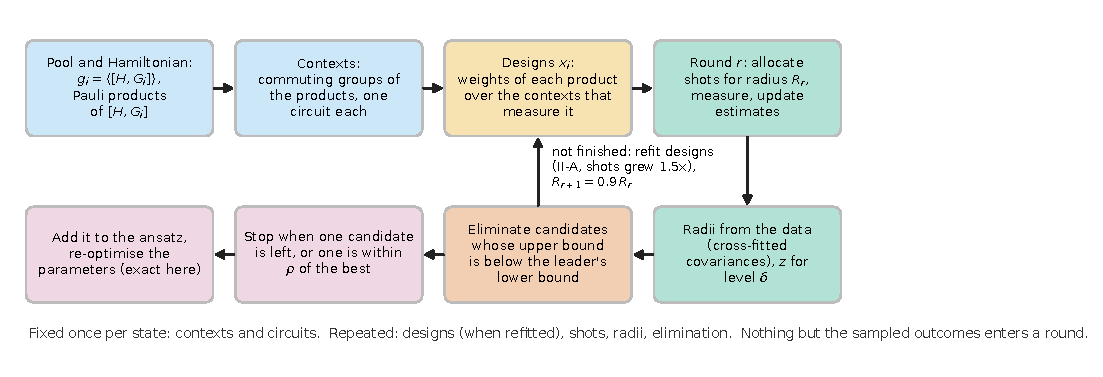
\includegraphics[width=0.92\textwidth]{figures/fig_pipeline}
\caption{One selection, in the order the method runs it. Contexts and circuits are fixed once per state; the designs, the shots, the radii and the elimination are repeated in every round, and nothing but the sampled outcomes enters a round.}
\label{fig:pipeline}
\end{figure*}

\subsection{Generator selection as a statistical decision}
\label{sec:decision}

At ADAPT iteration $k$ the state $\lvert\psi_k\rangle$ is fixed, and the pool $\mathcal A=\{\hat G_1,\dots,\hat G_K\}$ contains anti-Hermitian generators, $\hat G_i^\dagger=-\hat G_i$. The gradient operators
\begin{equation}
D_i=[\hat H,\hat G_i]
\end{equation}
are therefore Hermitian, and the gradients are their expectation values,
\begin{equation}
g_i=\langle\psi_k\rvert D_i\lvert\psi_k\rangle .
\end{equation}
The selection step must identify $i^\star=\arg\max_i\lvert g_i\rvert$. A candidate close enough to the best one,
\begin{equation}
\lvert g_i\rvert\ge\max_j\lvert g_j\rvert-\Delta ,
\label{eq:dgood}
\end{equation}
is called $\Delta$-good. The decision should be correct with probability at least $1-\delta$, with $\delta=0.05$ family-wise over the pool for all methods; Sec.~\ref{sec:elimination} states what the confidence intervals guarantee. Fixed-state benchmarks require exact identification. Along trajectories, where the leading gradient falls by more than an order of magnitude (from $0.3$ to $9\times10^{-3}$ on H$_4$), a selection may stop at a relative tolerance,
\begin{equation}
\lvert g_{\hat\imath}\rvert\ge(1-\rho)\max_j\lvert g_j\rvert ,\qquad \rho=0.1 ,
\label{eq:rhogood}
\end{equation}
where $\hat\imath$ is the generator returned by the selection. This tolerance is scale-free. The \emph{gap} of a state is the difference between its two largest $\lvert g_i\rvert$, and the \emph{relative gap} is the gap divided by the largest $\lvert g_i\rvert$. We report separately how often the exact best generator (ties included), a $\Delta$-good generator with $\Delta=1$ millihartree (mHa), and a $\rho$-good generator are selected. The cost of a selection is the number of context-shots needed to reach the decision, where one context-shot is one state preparation followed by one measurement in one measurement context.

\subsection{Shared Pauli representation of the gradients}
\label{sec:represent}

After the Jordan--Wigner mapping~\cite{jordanwigner1928}, every gradient operator is a linear combination of Pauli products. We write all of them in one common set of Pauli products $\{P_\ell\}_{\ell=1}^{L}$,
\begin{equation}
D_i=\sum_{\ell=1}^{L}A_{i\ell}P_\ell ,\qquad
\mu_\ell=\langle\psi_k\rvert P_\ell\lvert\psi_k\rangle ,\qquad
\boldsymbol g=A\boldsymbol\mu ,
\label{eq:Arep}
\end{equation}
where $A$ is a real $K\times L$ coefficient matrix built from the exact commutators; coefficients below $10^{-12}$ are dropped. The parent Pauli support of the selection step is
\begin{equation}
\mathcal B_0=\bigcup_{i}\operatorname{supp}(D_i),
\end{equation}
the set of all Pauli products that appear in at least one gradient: $1{,}276$, $30{,}196$ and $81{,}566$ products for H$_4$, LiH and H$_2$O.

Equation~\eqref{eq:Arep} is the reason measurements can be shared. Different commutators contain many of the same Pauli products (each product of $\mathcal B_0$ appears in $3.3$ to $4.0$ gradients on average), so one estimate of $\mu_\ell$ enters every gradient whose row of $A$ has a nonzero entry in column $\ell$. The same relation also makes the gradient estimates correlated, because they are built from the same measured data.

\subsection{Measurement contexts and sampling}
\label{sec:contexts}

\paragraph{Grouping.} Pauli products that commute qubit-wise (QWC) can be read out in a product basis~\cite{izmaylov2019,verteletskyi2020}, and fully commuting products with one Clifford circuit~\cite{yen2020}; both are the basis of measurement grouping for energy estimation. The Pauli products of $\mathcal B_0$ are partitioned into fully commuting (FC) parent contexts $\mathcal M_1,\dots,\mathcal M_N$ by deterministic first-fit insertion, a variant of sorted insertion~\cite{crawford2021} that sorts by Pauli weight instead of coefficient size: products are sorted by decreasing Pauli weight with lexicographic tie-breaking, and each joins the first context whose members it commutes with. This partition gives $N=53$ (H$_4$), $980$ (LiH) and $2{,}366$/$2{,}356$ (H$_2$O, equilibrium/stretched) contexts. No random numbers are used; other insertion orders (increasing weight, lexicographic, and seeded random orders) are used only to test robustness.

\paragraph{Measured groups.} A context is measured by a Clifford circuit $U_\alpha$ that maps $n_q$ independent commuting generators to the single-qubit operators $Z_q$. One shot therefore gives the eigenvalues of all $2^{n_q}$ elements of the maximal abelian group $\mathcal G_\alpha=\{\pm U_\alpha^\dagger Z^{\bm u}U_\alpha\}$, not only of the parent members. The generators of the parent members, of rank $\mathrm{rk}_\alpha\le n_q$, are completed to $n_q$ by adding products of $\mathcal B_0$ in decreasing order of coefficient mass $\sum_i\lvert A_{i\ell}\rvert$ that commute with the current generators and lie outside their span (a vector of the symplectic complement when none is left). A product $P_\ell$ is \emph{measured by} context $\alpha$ if $P_\ell\in\mathcal G_\alpha$, and its multiplicity is the number of contexts that measure it. With this completion each context reads on average $47$, $91$ and $107$ products of $\mathcal B_0$ (H$_4$, LiH, H$_2$O) instead of the $24$ to $35$ it was built from.

\paragraph{Diagonalization.} $U_\alpha$ is synthesized from the binary (GF(2)) tableau of the $n_q$ generators, which has an $X$ block and a $Z$ block: Hadamard gates on the non-pivot qubits make the $X$ block invertible, a change of generating set (no gates) brings it to the identity, which makes the $Z$ block symmetric, S and CZ gates clear the $Z$ block, and final Hadamard gates leave only $Z$ strings. Every product of interest is propagated through the gate list with its phase, $U_\alpha P_\ell U_\alpha^\dagger=s_\ell Z^{\bm u_\ell}$, so every bitstring gives the eigenvalue of every measured product. The number of CZ gates is recorded as the measurement-circuit cost; it averages $8.2$--$8.4$, $23.3$ and $32.2$ per context for H$_4$, LiH and H$_2$O. For $k$ independent generators on $n_q$ qubits, Ref.~\cite{crawford2021} gives a construction with at most $kn_q-k(k+1)/2$ two-qubit gates.

\paragraph{Sampling.} For a context $\alpha$ measured $m_\alpha$ times, the bitstring counts are sufficient statistics. One Walsh--Hadamard transform of the empirical distribution $\hat p_\alpha$ of the outcomes $\bm o\in\{0,1\}^{n_q}$ gives the means of all elements $Z^{\bm u}$ of the group,
\begin{gather}
\hat E_\alpha[\bm u]=\sum_{\bm o}\hat p_\alpha(\bm o)(-1)^{\bm u\cdot\bm o},\qquad
\hat\mu_\ell=s_\ell\hat E_\alpha[\bm u_\ell],\nonumber\\
\widehat{\operatorname{Cov}}(P_\ell,P_{\ell'})=s_\ell s_{\ell'}\big(\hat E_\alpha[\bm u_\ell\oplus\bm u_{\ell'}]-\hat E_\alpha[\bm u_\ell]\hat E_\alpha[\bm u_{\ell'}]\big),
\label{eq:moments}
\end{gather}
multiplied by $m_\alpha/(m_\alpha-1)$ for the unbiased sample covariance, and the exact distribution gives the exact moments through the same code. Different contexts use independent shots. In the simulations, the outcome distribution of each context is computed once from the state vector, and each batch of shots is one multinomial draw from it. All bitstring counts are stored, so any estimator can later be recomputed from the same data.

\subsection{Linear estimators and their covariance}
\label{sec:estimators}

\paragraph{Fragments and measurable operators.} For a fixed set of contexts, every linear unbiased estimator of the gradients can be written with context fragments $X_\alpha$,
\begin{equation}
\hat{\boldsymbol g}=\sum_\alpha X_\alpha\hat{\boldsymbol\mu}_\alpha ,\qquad
\sum_\alpha X_\alpha J_\alpha^{T}=A ,
\label{eq:recon}
\end{equation}
where $J_\alpha$ maps the products measured by context $\alpha$ into the full list of Pauli products. The second relation is the exact reconstruction condition: the fragments of each gradient must add up to $D_i$. Equivalently, each nonzero row of $X_\alpha$ defines a measurable operator $M_\beta=\sum_\ell\Omega_{\beta\ell}P_\ell$ supported in one measured group, and
\begin{equation}
D_i=\sum_\beta\Gamma_{i\beta}M_\beta ,\qquad A=\Gamma\Omega .
\end{equation}
Every design in this work, including every refit of a learned design, is checked for $\lVert A-\Gamma\Omega\rVert_{\max}\le10^{-9}\max\lvert A\rvert$, and a run fails if the check fails.

\paragraph{Covariance of the gradient estimates.} For any linear estimator of the form $\hat{\boldsymbol g}=\sum_\alpha X_\alpha\hat{\boldsymbol\mu}_\alpha$ (Eq.~\eqref{eq:recon}), with independent shots across contexts,
\begin{equation}
\begin{split}
\operatorname{Cov}(\hat{\boldsymbol g})&=\sum_\alpha\frac{1}{m_\alpha}X_\alpha\Sigma_\alpha X_\alpha^{T},\\
\operatorname{Var}(s_i\hat g_i-s_j\hat g_j)&=\boldsymbol d_{ij}^{T}\operatorname{Cov}(\hat{\boldsymbol g})\,\boldsymbol d_{ij},
\end{split}
\label{eq:cov}
\end{equation}
where $\boldsymbol d_{ij}$ has entries $s_i$ and $-s_j$ in positions $i$ and $j$. With shared contexts the off-diagonal terms are generally nonzero; when every gradient is measured in groups of its own, as in the independent baseline M2 of Sec.~\ref{sec:planning}, they vanish by construction. The covariance of the fragments of one context is built as the Gram matrix of centered fragment vectors, which is positive semidefinite and has the exact one-shot variances on its diagonal.

\subsection{Shared elimination and shot allocation}
\label{sec:elimination}

\paragraph{Confidence intervals and elimination.} All methods of this work, including the baselines of Sec.~\ref{sec:baselines}, share the confidence rule, the radius schedule and the stopping rule below, and differ only in what is measured and how shots are allocated. After each round, every active gradient $i$ has an estimate $\hat g_i$ and a standard error $\hat\sigma_i$. The confidence radius is $R_i=z\hat\sigma_i$, with a Bonferroni value $z=\Phi^{-1}\!\big(1-\delta/2K\big)$ over the $K$ gradients of the full pool ($z=3.10$, $3.46$ and $3.57$ for $K=26$, $92$ and $140$). This gives conservative lower and upper confidence bounds for the absolute gradients,
\begin{equation}
\mathrm{lcb}_i=\max\{0,\lvert\hat g_i\rvert-R_i\},\qquad \mathrm{ucb}_i=\lvert\hat g_i\rvert+R_i ,
\end{equation}
and candidate $i$ is eliminated when
\begin{equation}
\mathrm{ucb}_i<\max_{j\in\mathcal A_r}\mathrm{lcb}_j .
\label{eq:elim}
\end{equation}
Two sharper rules use the covariance of Eq.~\eqref{eq:cov}. The \emph{pairwise} rule eliminates $i$ when $\lvert\hat g_j\rvert-\lvert\hat g_i\rvert>z\operatorname{sd}(\hat s_j\hat g_j-\hat s_i\hat g_i)$ for some $j$, with signs $\hat s$ taken from the estimates. Because these plug-in signs are unreliable while a gradient is near zero, the \emph{sign-aware} rule uses a contrast only when the sign of the eliminating candidate is resolved, $\lvert\hat g_j\rvert>R_j$: candidate $i$ is eliminated when
\begin{equation}
\hat s_j\hat g_j-t\,\hat g_i>z\operatorname{sd}(\hat s_j\hat g_j-t\,\hat g_i),
\label{eq:safe}
\end{equation}
for $t=\hat s_i$ if the sign of $g_i$ is resolved, $\lvert\hat g_i\rvert>R_i$, and for both $t=\pm1$ otherwise. Given the sign of $g_j$, $\lvert g_j\rvert>\lvert g_i\rvert$ is equivalent to $s_jg_j>g_i$ and $s_jg_j>-g_i$, so the unresolved case needs no sign for $i$, and on the event that all intervals hold no step is wrong. The value of $z$ above covers one look per round. An \emph{anytime} variant spends $\delta_r=6\delta/(\pi^2r^2)$ in round $r$, which sums to $\delta$ over all rounds.

\paragraph{Radius schedule and stopping.} A run starts at radius $R_0$ and sets $R\leftarrow\gamma R$ every round, with $\gamma=0.9$ in the shot-level runs. The starting radius is either $\max_i\lvert g_i\rvert$, a mild oracle input, or the a priori bound $\max_i\sum_\ell\lvert A_{i\ell}\rvert\ge\lvert g_i\rvert$, which removes every exact quantity from the run. Each round allocates shots for the active set at the one-standard-error target $\epsilon=R/z$ by solving
\begin{equation}
\begin{split}
&\min_{\bm m}\sum_\alpha m_\alpha\quad\text{s.t.}\quad \operatorname{Var}(\hat g_i)=\sum_\alpha\frac{v_{i\alpha}}{m_\alpha}\le\epsilon^2\\
&\forall i\in\mathcal A_r,\qquad m_\alpha\ge c_\alpha ,
\end{split}
\label{eq:alloc}
\end{equation}
where $v_{i\alpha}$ is the one-shot variance of gradient $i$'s fragment in context $\alpha$ and $c_\alpha$ are the shots already taken (top-up accounting). This problem is solved by multiplicative dual ascent, $m_\alpha=\max\{c_\alpha,(\sum_i\lambda_iv_{i\alpha})^{1/2}\}$ and $\lambda_i\leftarrow\lambda_i(\operatorname{Var}_i/\epsilon^2)^{1/2}$, followed by the smallest feasible rescaling. Every context that carries a fragment receives at least one shot. A run stops when one candidate remains, when the radius falls below a floor ($10^{-3}R_0$ for the exact starting radius and $10^{-6}R_0$ for the a priori bound), or, if $\rho>0$, when the leader $\hat\imath$ is certified $\rho$-good against every survivor,
\begin{equation}
\begin{split}
&\hat s_{\hat\imath}\hat g_{\hat\imath}-(1-\rho)\,t\,\hat g_j>z\operatorname{sd}\big(\hat s_{\hat\imath}\hat g_{\hat\imath}-(1-\rho)\,t\,\hat g_j\big)\\
&t=\pm1,\ j\in\mathcal A_r\setminus\{\hat\imath\}.
\end{split}
\label{eq:rhostop}
\end{equation}
Elimination itself stays exact, so on the good event the best candidate survives and the returned one satisfies Eq.~\eqref{eq:rhogood}.

\paragraph{Shared elimination.} The estimators above are fixed, and the active set shrinks from the pool, $\mathcal A_0=\mathcal A$, as candidates are eliminated,
\begin{equation}
\mathcal A_0\supset\mathcal A_1\supset\cdots ,\qquad
\mathcal B_r=\bigcup_{i\in\mathcal A_r}\operatorname{supp}(D_i)\subseteq\mathcal B_0 .
\end{equation}
Only contexts that still carry a product of $\mathcal B_r$ are measured. The parent contexts are not rebuilt during a selection, so every earlier shot was taken in one of the same contexts and its bitstrings remain valid for the surviving gradients; they are pooled with the new ones. In each round the shots are allocated by Eq.~\eqref{eq:alloc}, with the pairwise rule, $\gamma=0.9$ and top-up accounting, and the selection ends by the stopping rule above. We call this procedure \emph{shared elimination with fixed estimators}, or II-0 in the hierarchy of Sec.~\ref{sec:design}. Its planning-bound form with exact gradients and variances, M3, is defined in Sec.~\ref{sec:baselines}.

\subsection{Redesigning the measurable estimators}
\label{sec:design}

\paragraph{Hierarchy of designs.} The levels below add one degree of freedom at a time.
\begin{description}
\item[II-0.] Fixed fragments on the parent contexts, with shots allocated by Eq.~\eqref{eq:alloc} in every round: the shared elimination of Sec.~\ref{sec:elimination}.
\item[II-A.] Coefficient splitting. A product measured by several contexts may carry part of its coefficient in each, and the split is chosen to lower the variance~\cite{yen2023}. The overlap comes from the completed measured groups; no context is enlarged.
\item[II-B.] Zero-sum augmentation. Products of $\mathcal B_0$ with $A_{i\ell}=0$ that are measured by at least two contexts already carrying $D_i$ are added with coefficients that sum to zero over contexts, so they cancel in Eq.~\eqref{eq:recon} but can lower the variance through their covariance with the required products~\cite{choi2022}. At most 200 candidates per gradient are kept, ranked by the single-context control-variate score $\sum_\alpha\operatorname{Cov}(F^{(0)}_{i\alpha},P_\ell)^2/\operatorname{Var}(P_\ell)$, where $F^{(0)}_{i\alpha}$ is the II-0 fragment.
\item[II-C.] Dictionary design. Contexts with a small shot share are removed when every required product they contain is measured elsewhere, and each context block is compressed to its rank, which gives the smallest set of measurable operators $M_\beta$. 
\item[II-D.] BAI-adaptive redesign. The design is recomputed for the surviving rows of $A$ . In oracle form, design and allocation are reoptimized jointly at every elimination breakpoint, which gives a ceiling. In learned form, the II-A coefficients of the active candidates are refit from the measured data (Sec.~\ref{sec:cov}) whenever the shots held have grown by a factor of 1.5.
\item[II-E.] Direct contrast design. As II-D, but the estimators of the contrasts between the leader and each challenger are designed directly, and both the allocation and the elimination use these contrasts (see below).
\end{description}

\paragraph{Minimum-variance split.} For fixed contexts, covariances $\Sigma_\alpha$ and shots $m_\alpha$, the variance of $\hat g_i$ is the convex quadratic $\sum_\alpha\boldsymbol x_{i\alpha}^T\Sigma_\alpha\boldsymbol x_{i\alpha}/m_\alpha$ of gradient $i$'s coefficients. Products measured in only one context keep their coefficient from $A$. Writing $\boldsymbol x_i=\boldsymbol x_i^{(0)}+W\boldsymbol y$, with $\boldsymbol x_i^{(0)}$ the II-0 coefficients and the columns of $W$ the moves that shift weight between two copies of one product (or between copies of an auxiliary product), the optimum solves
\begin{equation}
\big(W^TQW\big)\boldsymbol y=-W^TQ\,\boldsymbol x_i^{(0)},\qquad Q=\bigoplus_\alpha\Sigma_\alpha/m_\alpha ,
\label{eq:gls}
\end{equation}
by a sparse direct solve. The result is the generalized least-squares, best linear unbiased estimator of $D_i$ among the splits generated by these moves. If every product measured in a context may carry a coefficient, it is the best linear unbiased estimator in the full class, and by the Gauss--Markov theorem the same estimator is optimal for every linear combination of the gradients at the same shots, so that changing the target changes only the shot allocation. The moves of II-A are restricted to the products that a gradient requires, so a combination in which the coefficient of a product cancels has a larger set of moves, and the best split of a contrast can then differ from the difference of the two gradient splits; the direct contrast design of II-E exploits this.

\paragraph{Objectives and shot allocation.} The levels differ in the precision targets imposed in Eq.~\eqref{eq:alloc}. II-0 to II-D require $\operatorname{Var}(\hat g_i)\le\epsilon^2$ for every active candidate. At fixed shots the gradients decouple, so this also minimizes any weighted sum of the variances $\operatorname{Var}(\hat g_i)$ with nonnegative weights. Each generator's problem is a convex quadratic over the copies of its Pauli products. II-E instead requires
\begin{equation}
\operatorname{sd}\big(\hat s_{\hat\imath}\hat g_{\hat\imath}-t\,\hat g_j\big)\le2\epsilon\quad\text{for every survivor } j,\qquad \operatorname{sd}(\hat g_{\hat\imath})\le\epsilon ,
\label{eq:contrastalloc}
\end{equation}
the separation that two candidates resolved to radius $\epsilon$ would certify, and the leader's own precision for sign resolution. The BAI decision is set by the hardest pair, so a natural objective is
\begin{equation}
\min\;\max_{j\in\mathcal A_r\setminus\{\hat\imath\}}\operatorname{Var}(s_{\hat\imath}\hat g_{\hat\imath}-s_j\hat g_j),
\end{equation}
subject to exact reconstruction and a shot budget. Because Eq.~\eqref{eq:alloc} is scale-free, minimizing the total shots under the constraints of Eq.~\eqref{eq:contrastalloc} is the epigraph form of this min--max objective at a fixed budget. 

\paragraph{Contrast elimination.} Once the sign of the leader is resolved, $\lvert\hat g_{\hat\imath}\rvert>R_{\hat\imath}$, II-E gives each survivor $j$ a cross-fitted estimator of $\hat s_{\hat\imath}g_{\hat\imath}-t\,g_j$, with $t=\hat s_j$ if $j$'s sign is resolved and both $t=\pm1$ otherwise. The estimator is designed directly over the union of both gradients' coordinates: products whose coefficients cancel become zero-sum control variates, and the fallback is the difference of the two gradient designs. Challenger $j$ is eliminated when the lower confidence bound of
\begin{equation}
\lvert g_{\hat\imath}\rvert-\lvert g_j\rvert=\min_{t\in\{\pm1\}}\big(s_{\hat\imath}g_{\hat\imath}-t\,g_j\big)
\end{equation}
is positive, which is Eq.~\eqref{eq:safe} with the designed contrasts, and the run stops by Eq.~\eqref{eq:rhostop}.

\paragraph{Which parts are convex.} For a fixed context library and fixed covariances, each term $\boldsymbol x^{T}\Sigma_\alpha\boldsymbol x/m_\alpha$ is quadratic-over-linear and therefore jointly convex in the fragment coefficients and $m_\alpha>0$, and the reconstruction condition Eq.~\eqref{eq:recon} is linear. The fragment-and-allocation problem is therefore convex. Alternating Eq.~\eqref{eq:gls} with Eq.~\eqref{eq:alloc} is monotone but stalls once a context's shots reach zero. The oracle designs therefore eliminate $\bm m$ analytically and solve the saddle problem $\min_{\bm x}\max_{\bm\lambda\ge0}\sum_\alpha\varphi(\sum_i\lambda_iv_{i\alpha})-\epsilon^2\sum_i\lambda_i$, with $\varphi(\xi)=m+\xi/m$ and $m=\max(c_\alpha,\sqrt\xi)$. The oracle designs use smoothed L-BFGS over all active coefficients and multiplicative dual ascent, and the reported cost is the exact allocation of the returned design. The problem becomes combinatorial when the membership of the contexts is chosen, and bilinear and generally non-convex when both $\Gamma$ and $\Omega$ of the dictionary are optimized. For this reason the context library is fixed within a selection.

\paragraph{Solving the split for large libraries.} The split of Eq.~\eqref{eq:gls} has one unknown per extra copy of a Pauli product in the contexts of the gradient. On the fully commuting contexts this number is small, but on the QWC contexts of H$_2$O a Pauli product has $15$ copies on average (up to $7{,}000$) and the problem has up to $10^5$ unknowns per generator. When the primal problem would exceed $12{,}000$ unknowns or $5\times10^{7}$ Hessian entries we therefore solve the same minimization in its dual, with one unknown per Pauli product (about $1{,}200$ per generator on H$_2$O). The switch never occurs on the fully commuting or reuse libraries, so their results do not depend on it. On LiH the two formulations reach the same variance to $3\times10^{-8}$, though not always the same coefficients where the variance is flat, and the mean cost of II-A on the QWC contexts of two LiH states agrees to $1.3\%$ for both rules over $100$ trials each, within the statistical error of about $2\%$.

\subsection{Learning covariances from measurements}
\label{sec:cov}

The designs above require the covariances $\Sigma_\alpha$ of the measured state, which are not known before measuring. We call a design \emph{learned} when its covariances are estimated from the shots taken so far. We use two sources, a prior and the data, and combine them by shrinkage.

\paragraph{Classical prior.} The prior is either the covariance of the Hartree--Fock determinant in the problem's own orbital basis or a flat prior (unit variances, no correlation). It is only a starting point and is never treated as exact for the measured state.

\paragraph{Empirical covariance.} The unbiased sample covariance $\hat\Sigma_\alpha$ of Eq.~\eqref{eq:moments} from the accumulated bitstring counts of context $\alpha$. This estimate is positive semidefinite, so no ridge or projection is needed.

\paragraph{Shrinkage.} The design uses
\begin{equation}
\tilde\Sigma_\alpha=\omega_\alpha\Sigma^{\mathrm{prior}}_\alpha+(1-\omega_\alpha)\hat\Sigma_\alpha ,\qquad
\omega_\alpha=\frac{\nu}{\nu+m_\alpha},
\end{equation}
so the weight of the prior falls as the context collects shots. Here $\nu$ is the effective number of shots assigned to the prior; we test $\nu\in\{0,100,1000,\infty\}$, and the headline runs use $\nu=0$ (data only).

\paragraph{Cross-fitting.} Choosing an estimator from the same data that it then averages can bias the estimate. Instead of freezing designs batch by batch, we use cross-fitting~\cite{chernozhukov2018}: every context's shots are split into two folds; the design fitted on fold $f$ is applied to the means of the other fold $\bar f$, and the two half-estimates are averaged. Each half-estimate is unbiased whatever its design, conditional on the shots held, so designs can be refit at any time and all data enter every estimate. The shots of later rounds are allocated from earlier outcomes, so in the sequential procedure unbiasedness and the confidence intervals are approximate, and Q3 and Q4 report how well they hold. The confidence radii and the allocation use only the held-out fold: given the fitted designs, the two half-estimates are independent, and
\begin{equation}
\operatorname{Cov}(\hat g_i,\hat g_j)=\tfrac14\sum_{f}\sum_\alpha\boldsymbol x^{f\,T}_{i\alpha}\tilde\Sigma^{\bar f}_\alpha\boldsymbol x^{f}_{j\alpha}/m^{\bar f}_\alpha ,
\end{equation}
because a covariance that includes the fitting fold underestimates the variance of the design fitted to it. Three safeguards complete the procedure:
\begin{enumerate}[label=(\roman*)]
\item a context carries learned coefficients only once both folds hold at least 50 shots in it;
\item a fitted design is kept for gradient $i$ only if the held-out fold predicts a lower variance than the II-0 coefficients;
\item a held-out covariance from fewer than 50 shots is replaced, for the radii and the allocation alike, by $\kappa\,\mathbb 1$ over its $\kappa$ products, a valid upper bound because $\Sigma\preceq\operatorname{tr}(\Sigma)\,\mathbb 1\preceq\kappa\,\mathbb 1$.
\end{enumerate}
The first round is an II-0 pilot, and designs are refit for the active candidates whenever the shots held have grown by a factor of 1.5.

\paragraph{Oracle and empirical modes.} All headline results use the empirical mode, in which every decision is made from the classical prior and the measured data only, with one exception: the fixed-state runs start from $R_0=\max_i\lvert g_i\rvert$ unless marked as using the a priori $R_0$. Exact gradients and exact covariances of the state are used only in an oracle mode, to score the runs and to compute reference variances, and they are stored in separate validation records; with the a priori starting radius no exact quantity enters a run. A design that uses exact covariances is always labeled as oracle.

\subsection{Operator pool}

The pool is the spin-orbital unitary coupled-cluster singles and doubles (UCCSD) pool built on the Hartree--Fock reference,
\begin{equation}
\{\hat a_{\mathrm v}^\dagger\hat a_{\mathrm o}-\hat a_{\mathrm o}^\dagger\hat a_{\mathrm v} ,\;
\hat a_{\mathrm v}^\dagger\hat a_{\mathrm v'}^\dagger\hat a_{\mathrm o'}\hat a_{\mathrm o}-\hat a_{\mathrm o}^\dagger\hat a_{\mathrm o'}^\dagger\hat a_{\mathrm v'}\hat a_{\mathrm v}\},
\end{equation}
where $\mathrm o,\mathrm o'$ label occupied and $\mathrm v,\mathrm v'$ virtual spin orbitals, with $K=26$, $92$ and $140$ generators for H$_4$, LiH and H$_2$O. The generators conserve the electron number and $S_z$, but not the total spin $S^2$. The generators are mapped to qubits with the Jordan--Wigner transformation. 

\subsection{ADAPT trajectories}

Fixed-state benchmarks use the Hartree--Fock determinant and the configuration-interaction singles-and-doubles (CISD) ground state of each geometry, the lowest eigenstate of the Hamiltonian within the determinants up to double excitations of the Hartree--Fock determinant, and, in addition, states saved along exact ADAPT trajectories: $\lvert\psi_k\rangle$ after $k$ generators, grown from Hartree--Fock by the exact largest $\lvert g_i\rvert$ (ties to the lowest index) with all parameters reoptimized. The gradient problem of a saved state is built from the same Hamiltonian object as the trajectory, so that orbital phases, and hence gradient signs, are consistent. In a \emph{measured} trajectory every selection is made by a method from sampled outcomes on the current state, fully in the empirical mode (estimated radii, a priori starting radius, sign-aware rule, $\rho=0.1$), and the ansatz grows with that choice.

\subsection{VQE parameter optimization}

After a generator is selected, all parameters are reoptimized together with the BFGS algorithm in \texttt{scipy.optimize.minimize}~\cite{virtanen2020}. Energies and analytic gradients are exact, computed in the $(n_\uparrow,n_\downarrow)$ sector of the spin-up and spin-down electron numbers (36, 225 and 441 determinants), and the gradient tolerance is $10^{-9}$. Because the Hamiltonian and the generators conserve both numbers, the state stays in this sector, and its Pauli expectation values are those of the full qubit space used in the selection step. The new parameter starts at zero and the others at their previous values. Only the selection step is measured with simulated shots, sampled from the exact outcome distribution without device noise; the optimization is exact, so that differences between methods come from selection alone. A run stops when the energy is within chemical accuracy, $1.6$~mHa, of the full configuration interaction (FCI) energy in the same basis, when every $\lvert g_i\rvert<10^{-6}$, or after ten iterations beyond the exact trajectory.

\subsection{Resource accounting}
\label{sec:resources}

We count the following quantities separately:
\begin{itemize}
\item \emph{Context-shots}, the main cost. One context-shot is one state preparation and one measurement in one context, so the number of state preparations equals the number of context-shots.
\item \emph{Measurement-circuit cost}, the number of two-qubit gates of each diagonalizing Clifford circuit, reported per circuit and weighted by the shots it receives. Fewer shots are not an advantage if the circuits become much deeper.
\item \emph{Classical design time}, the time spent building designs, statistics and allocations, logged per run.
\item \emph{Parameter-optimization measurements}, estimated with a cost model. At iteration $k$ with $n_k$ parameters, the exact optimizer used $n_k^{\mathrm{ev}}$ evaluations of energy and gradient. Each evaluation is counted as one energy estimate plus a parameter-shift gradient~\cite{mitarai2018,schuld2019} with $\eta$ energies per parameter, where $\eta=2$ to $4$~\cite{kottmann2021}. Each energy estimate has a standard error $\varepsilon_E=1$~mHa and uses fully commuting groups of $\hat H$ formed by sorted insertion~\cite{crawford2021} (4 groups for H$_4$ and 39--42 for LiH, depending on the self-consistent-field (SCF) solution within degenerate orbitals) with optimal allocation~\cite{rubin2018}, which costs $m_E=(\sum_\alpha\sigma_\alpha)^2/\varepsilon_E^2$ context-shots, with $\sigma_\alpha$ evaluated at the optimized state of the iteration. The optimization cost is then
\begin{equation}
C_{\mathrm{opt}}=\sum_k n^{\mathrm{ev}}_k\,(1+\eta\,n_k)\,m_E^{(k)} .
\end{equation}
\end{itemize}
The total measurement cost of an ADAPT run is written as $C_{\mathrm{ADAPT}}=C_{\mathrm{sel}}+C_{\mathrm{opt}}$. If selection becomes $s$ times cheaper, the end-to-end speedup is
\begin{equation}
S_{\mathrm{total}}=\frac{C_{\mathrm{sel}}+C_{\mathrm{opt}}}{C_{\mathrm{sel}}/s+C_{\mathrm{opt}}} .
\label{eq:stotal}
\end{equation}
The cost model uses the exact optimizer's evaluation counts and no reuse of shots between evaluations, so $C_{\mathrm{opt}}$ is likely an underestimate.

\paragraph{Implementation.} Every finite-shot trial uses its own random stream, so results do not depend on how trials are distributed over processes or machines. The code is tested against dense linear algebra (commutators, gradients, fragment covariances, circuit images) and by 140 unit tests. The sampler reproduces the analytic means, variances and correlations within statistical tolerance down to $86$ shots in total. All tables are regenerated from stored per-trial outputs by the scripts in the repository; cluster runs are checkpointed per trial and resume exactly.

\subsection{Benchmark settings and edge cases}
\label{sec:settings}

\paragraph{Method definition and benchmark settings.} The estimators, the elimination rules and the allocation of Eq.~\eqref{eq:alloc} define the method. The following values are settings of the benchmark and change the cost, not the definition: the confidence $\delta=0.05$, the radius schedule $\gamma=0.9$, the tolerance $\rho=0.1$, the prior weight $\nu=0$, the first-fit insertion order, and the starting radius $R_0$ (the exact largest gradient, or the a priori bound). We tested the effect of $\gamma$ (Q3), of $\nu$ (Q4), of the insertion order (Q3) and of the radius (Discussion). The thresholds of 50 shots and the refit factor of 1.5 were fixed and are varied in Q11; the cap of 200 auxiliary candidates per gradient belongs to the zero-sum auxiliary products of Q4, which the II-A results do not use, and was not varied.

\paragraph{Edge cases.} The procedure is defined when its preferred assumptions fail. Exactly tied leaders are never separated by elimination, so a selection with $\rho=0$ ends only at the radius floor, and with $\rho>0$ it returns any candidate certified $\rho$-good. A context with fewer than 50 shots per fold carries no learned coefficients, and a held-out covariance from fewer than 50 shots is replaced by the bound $\kappa\,\mathbb 1$. A learned design is kept for a gradient only if its predicted held-out variance is lower than that of the fixed design, so the method falls back to II-0 per gradient; a design that fails the reconstruction check stops the run. The selection step does not decide whether the run should stop: when all gradients are close to zero it ends at the radius floor, and the cost of certifying termination is a separate problem (Discussion).

\section{Baselines and additional measurement settings}
\label{sec:baselines}

The comparisons of the Results use the reference strategies of Sec.~\ref{sec:planning}, evaluated as planning bounds with exact gradients and variances, and published baselines run from sampled outcomes (Sec.~\ref{sec:external}). Sec.~\ref{sec:depth} defines context families of lower circuit depth and the noisy measurement circuits of the Discussion.

\subsection{Reference strategies and planning bounds}
\label{sec:planning}

\paragraph{Planning bounds.} M1--M3 are also evaluated as oracle planning bounds, with exact gradients and fragment variances: in the limit $\gamma\to1$ candidate $i$ leaves at radius $\Delta_i/2$, with $\Delta_i=\lvert g_{(1)}\rvert-\lvert g_i\rvert$ and $\lvert g_{(1)}\rvert=\max_j\lvert g_j\rvert$, and each context is charged the largest request it receives. M3 is additionally evaluated eliminating on each candidate's actual precision, which on a shared allocation is better than the common radius. A finite-shot surrogate draws Gaussian estimates with these variances; all other finite-shot results sample measurement outcomes.

\paragraph{M1: FC-UG.} Fully commuting universal groups for all-gradient estimation. One allocation, Eq.~\eqref{eq:alloc} with $c=0$, over all $K$ gradients at the common radius $\mathrm{gap}/2$ (fixed states) or $\rho\max_i\lvert g_i\rvert/2$ (trajectories), which certifies the winner or a $\rho$-good candidate. M1 is handed the exact gap or scale and therefore represents static estimation at its best.

\paragraph{M2: BAI-FC-IG.} Best-arm identification with fully commuting individual-gradient groups. Each gradient is one arm and is measured independently: the support of each $D_i$ is grouped by the same first-fit routine into $N_i$ own groups, and within an arm shots follow the optimal independent-fragment allocation~\cite{rubin2018,crawford2021}, which costs $(\sum_\alpha\sigma_{i\alpha})^2/\epsilon^2$ shots for standard error $\epsilon$, with $\sigma_{i\alpha}$ the standard deviation of the arm's fragment in group $\alpha$. Arms are eliminated with Eq.~\eqref{eq:elim}. M2 uses elimination but no sharing between gradients, so it isolates the benefit of BAI alone. A \emph{no-sharing baseline}, every gradient grouped separately and resolved to M1's radius, completes the $2\times2$ factorial of sharing and elimination.

\paragraph{M3: BAI-FC-UG.} Best-arm identification with fully commuting universal groups: the shared elimination of Sec.~\ref{sec:elimination} evaluated as a planning bound. M3 uses the same parent contexts as M1 together with elimination, and its shot-level implementation is II-0.

\paragraph{Shot reuse.} To measure how much sharing a method achieves, we define its reuse as the average number of surviving candidates informed by one context-shot, accumulated over the whole selection, $\sum_r\sum_\alpha m^{(r)}_\alpha\,\lvert\{i\in\mathcal A_r:\alpha\ \text{carries a fragment of}\ i\}\rvert/\sum_{r,\alpha}m^{(r)}_\alpha$, evaluated from logged runs. M2 has a reuse of one by construction.

\subsection{External baselines at shot level}
\label{sec:external}

The planning bounds above use exact gradients and variances. For the comparison with the published baselines (Sec.~\ref{sec:q8}) each baseline is also run like the methods of this work: from sampled measurement outcomes, with the confidence rule, radius schedule and stopping rule of the previous subsection, and with variances estimated from the shots wherever the corresponding method of Sec.~\ref{sec:design} estimates them.

\paragraph{M1, static and sequential.} \emph{M1 static} is the planning allocation of M1 with sampled outcomes: one allocation for the whole pool at the radius $\mathrm{gap}/2$ (fixed states) or $\rho\max_i\lvert g_i\rvert/2$ (trajectories), computed from the exact fragment variances, one multinomial draw per context, and the largest estimate is returned. It is handed the exact gap and variances and treats the estimates as independent. \emph{M1 seq} is the sequential, non-oracle form of all-gradient estimation: the same parent contexts, one common precision for every gradient that shrinks by $\gamma$ per round, and the rule, stopping condition and estimated covariances of II-0, but \emph{no elimination}. Every gradient stays in the allocation; the rule only decides when to stop, so a candidate that it has removed no longer takes part in the comparisons but is still measured. M1 seq therefore uses the covariance of the shared estimates and isolates the benefit of elimination.

\paragraph{M2, sampled.} Every gradient is one arm with its own fully commuting groups, as in the planning form of M2 above. A group is measured in one Clifford circuit, so the fragment of an arm is a known function $e_\alpha(\bm o)$ of the outcome $\bm o$, and $\sum e$ and $\sum e^2$ over the shots of the group are sufficient statistics. The shots of an arm follow the optimal independent allocation $m_\alpha\propto\hat\sigma_\alpha$, topped up from the shots held. A group with fewer than 50 shots uses the Popoviciu bound $\sigma_\alpha\le(\max e_\alpha-\min e_\alpha)/2$, which needs no data. Elimination uses the rules of the previous subsection on the independent estimates: the absolute-interval rule is Successive Elimination~\cite{evendar2006} on $\lvert g\rvert$ in the formulation of Huang and Izmaylov~\cite{huang2026}, with the confidence radii of this work in place of their hand-set radius, a fixed multiple of the precision target of each round, which carries no stated confidence level.

\paragraph{Reuse of the energy measurement.} We model the scheme as described in the arXiv version (v1, July 2025) of Ref.~\cite{ikhtiarudin2025}; the published version, which has a different title, was not re-implemented. Ikhtiarudin \textit{et al.} save the Pauli outcomes of the last VQE energy evaluation of an ADAPT iteration and reuse them for the Pauli products of $[\hat H,\hat G_i]$ that share a measurement basis with a clique of $\hat H$, and they allocate shots by variance over QWC cliques~\cite{ikhtiarudin2025}. We model this as follows. The groups of $\hat H$ (fully commuting by sorted insertion~\cite{crawford2021} in decreasing coefficient $\lvert h_P\rvert$ of the Pauli terms $P$ of $\hat H$, the grouping of the $C_{\mathrm{opt}}$ model, or QWC cliques, measured in a product basis) are added to the context library as \emph{energy contexts}. The energy contexts hold the shots of one energy estimate to a standard error $\varepsilon_E$, allocated optimally and drawn once per trial from the state; $\varepsilon_E=1$~mHa as in $C_{\mathrm{opt}}$. These shots are part of $C_{\mathrm{opt}}$ and are not charged to the selection. Every Pauli product that an energy context measures (its whole maximal group, not only the terms of $\hat H$) is read from the best-funded such context, all others from their parent context. The selection is all-gradient estimation (M1 seq), and new shots are allocated by the optimal allocation of Eq.~\eqref{eq:alloc}, which is at least as good as their variance-minimizing or variance-preserving rules.

\paragraph{Reuse by the new methods, and controls.} To separate the effect of the data from that of the grouping, the QWC variant is also run without the free data. We give II-0 and II-A the same free data on the same library (``II-0 + reuse'', ``II-A + reuse''); II-A may then split a coefficient between an energy context and a parent context. II-A is run with the forced assignment above and from the home design, where the learned splitting alone decides whether to use the energy contexts; the comparison tables report the better variant per state, as the baseline gets the better of its fully commuting and QWC versions. The control without free data uses plain home assignment on the same grouping. The cached Hamiltonian terms are used only after the rebuilt Hamiltonian has reproduced the energy of the state and the stored commutators $[\hat H,\hat G_i]$ of all generators, because a different orbital choice within a degenerate shell changes the Pauli support, and with it the overlap that reuse exploits.

\paragraph{Informationally complete measurements.} AIM-ADAPT-VQE measures every qubit with a single-qubit informationally complete (IC) positive operator-valued measure (POVM) and estimates the energy and all commutators from the same data~\cite{nykanen2025}. We simulate the data model exactly with the product of tetrahedral, or symmetric informationally complete (SIC), POVMs, which is the unoptimized member of the family: the outcome distribution on all $4^{n_q}$ outcomes, the exact single-shot estimator of every gradient (a Pauli product of weight $w$ has second moment $3^w$) and its exact covariance. The cost is the number of IC shots until the same rules certify the decision, with radii from the exact covariance or from the sample covariance. The adaptive optimization of the POVM parameters of the paper, which lowers the variance of the energy, is not modeled, so the numbers are an upper bound for the optimized scheme. An IC shot measures all qubits in the IC POVM, so IC shots and context-shots are different resources, and only statistical efficiency is compared.

\paragraph{Operator pools.} Besides the spin-orbital UCCSD pool we use the pools of the ADAPT literature that give the Pauli structure of the gradients a different shape: qubit-ADAPT~\cite{tang2021} (each Pauli string of the Jordan--Wigner image of a UCCSD generator, with its $Z$ operators removed, as its own generator), qubit-excitation (QEB) generators~\cite{yordanov2021} with the UCCSD index sets, and, with generalized index sets (all spin-conserving singles and doubles among all spin orbitals), generalized QEB, generalized qubit-ADAPT and the one-variational-parameter coupled exchange operators (OVP-CEO) of CEO-ADAPT-VQE~\cite{ramoa2025ceo}. On four spin orbitals (two spin-up, two spin-down) the two qubit excitations give the two CEOs, their sum and their difference; on four orbitals of one spin the three qubit excitations give six CEOs; singles are qubit excitations. The Hamiltonian, state and pipeline are those of the UCCSD pool. The symmetry-adapted minimal complete pool of Ref.~\cite{shkolnikov2023} is not included.

\paragraph{Pivot grouping.} Anastasiou \textit{et al.}~\cite{anastasiou2023} do not group the support of all gradients at once. Their pivot is one Pauli term $P$ of $\hat H$ with coefficient $h_P$, and for pool strings $S$ and $S'$ that commute with each other the commutators $[P,S]$ and $[P,S']$ commute too, since $[[P,S],[P,S']]=4[S',S]=0$. The pool strings are partitioned once into commuting classes (the $2n_q$ anchored classes ($n_q$ qubits) of the qubit-type pools, in which every string has its single $Y$, or its single $X$, on one qubit; first-fit classes for the UCCSD pool), and the contexts are the pairs (pivot, class); their diagonalizing circuits need at most $n_q-3$ CNOT gates in the original construction. Ikhtiarudin \textit{et al.}\ report, in the published version of their work~\cite{ikhtiarudin2025}, that this grouping alone gives the dominant reduction of the shots of the gradient step.

\paragraph{Pivot contexts as implemented.} We build the contexts for every pool of this work and read every Pauli product of a gradient from the context of the pivot that produced it, with the coefficient it had there (``pivot, as published''): a product that arises from several pivots is then measured, and its variance paid, in each of them. Because a UCCSD gradient is a sum of up to eight strings this is wasteful, so we also give the baseline the option of reading each product from one pivot context, chosen by a greedy set cover (``pivot, merged''), which is stronger than the published scheme. The shots follow the optimal allocation of Eq.~\eqref{eq:alloc} with exact (static) or estimated (sequential) variances, not their bound $\operatorname{Var}\le1$, and the circuits are synthesized generically, so their gate counts bound those of the original construction from above. The decomposition of every commutator into pivot contributions is checked against the stored expansion to $10^{-8}$, and on the qubit pool the cost of M1 static at a common precision $\epsilon=10^{-2}$ is $34.8\,(\sum_P\lvert h_P\rvert)^2/\epsilon^2$ on H$_4$, against the $4n_q=32$ of their analysis.

\paragraph{M2 with QWC fragments.} Huang and Izmaylov fragment each commutator into qubit-wise commuting groups by sorted insertion~\cite{huang2026,crawford2021}. ``M2 QWC'' is M2 with these groups in place of the fully commuting ones, with the estimated variances, the radii and the rules of this work: product measurements, no entangling gates.

\subsection{Context families of lower depth, and noisy circuits}
\label{sec:depth}

Fully commuting contexts need $8$--$32$ two-qubit gates per circuit on average (Q1). To see what the shots cost at lower depth, Pauli products are also grouped so that they commute \emph{block by block}: two Paulis are compatible when their restrictions to every block of a partition of the qubits commute, and the circuit of a group is a tensor product of one Clifford per block, with at most $b(b-1)/2$ CZ gates per block of $b$ qubits. Blocks of one qubit are qubit-wise commutation (product measurements, no entangling gate), blocks of all qubits are the fully commuting grouping of Sec.~\ref{sec:contexts}. We use consecutive blocks of $1$, $2$ and $4$ qubits, which in Jordan--Wigner order pairs the two spins of one spatial orbital and two spatial orbitals. Groups are formed by the same first-fit insertion as for the fully commuting contexts, every method of this work runs on every family unchanged, and the QWC cliques of the reuse baseline are measured in a product basis in the same way (the Pauli products a context measures are those of its local basis).

To see what depth costs when the gates are imperfect we make the measurement circuits noisy in the way that stays exact for Clifford circuits. After every CZ gate a two-qubit depolarizing channel of total error probability $p_2$ acts, and every readout is flipped with probability $p_{\mathrm{ro}}$ (zero unless stated). A Pauli observable, propagated back through the circuit, is multiplied by $1-16p_2/15$ at every CZ gate at which it is not the identity on the two qubits, and by $(1-2p_{\mathrm{ro}})$ per qubit of its $Z$-string at the readout; the noisy outcome distribution of a context is the one whose group means are the damped ones. This damping agrees with a density-matrix simulation of the channels to $10^{-12}$ (unit test). The estimators and intervals are those of the noiseless study and know shot noise only, and a selection counts as correct if it picks the best generator of the \emph{noiseless} gradients.

\section{Results}

The benchmarks are square H$_4$ (side $1.0$ and $2.0$~\AA, 8 qubits), LiH (Li--H distance $3.0$~\AA, 12 qubits) and H$_2$O (O--H distance $0.9572$ and $1.75$~\AA, 14 qubits) in the STO-3G basis~\cite{hehre1969}, with the Hartree--Fock (HF) and CISD states of each geometry (LiH: HF only) and states saved along exact ADAPT trajectories. The CISD state stands for the correlated states late in an ADAPT run, where the gradients are small and the selection is expensive (Q2). The systems cover three scales of the selection problem: H$_4$ is the smallest (8 qubits, 26 generators), LiH has a pool of 92 generators, and H$_2$O has 140 generators and $81{,}566$ Pauli products. The stretched geometries are included because stretching crowds the top of the gradient spectrum, which makes the selection harder (Q2). The questions follow the argument of the Introduction. Q1--Q3 ask whether sharing and elimination each reduce the cost and whether they compound, using planning bounds with exact variances. Q4 and Q5 ask what the learned estimators add when everything is estimated from the shots. Q6 and Q7 ask whether the saving survives in a complete ADAPT run and whether selection is still the dominant cost. Q8 asks how the result compares with the published strategies, run under the same rules. Costs are context-shots at $\delta=0.05$, for the UCCSD pool unless another pool is named. Planning bounds use exact gradients and variances and are labeled as such; all other results sample measurement outcomes, with 100--250 trials per configuration (means, with medians where a tail dominates). LiH trajectory-state, H$_2$O finite-shot and H$_2$O trajectory runs were carried out on a cluster. Measured ADAPT trajectories were run on all three molecules; those of H$_2$O appear in Q8.

\subsection{Q1: Does sharing help? Alone, only by a factor of 1--3}

\begin{table}[!htb]
\centering\small
\caption{Shared measurement structure. $N$: parent FC contexts; $\sum_iN_i$: contexts of the per-gradient groupings (M2); uses: average number of gradients in which a product of $\mathcal B_0$ appears; multiplicity and split.: number of contexts whose measured group contains a product of $\mathcal B_0$, and the share of $\mathcal B_0$ measured at least twice; CZ: two-qubit gates per diagonalizing circuit; sharing: cost of the no-sharing baseline over M1 (planning bound).}
\label{tab:q1}
\footnotesize\setlength{\tabcolsep}{3.5pt}
\fitcol{%
\begin{tabular}{lrrrrr}
\toprule
System & qubits & $K$ & $\lvert\mathcal B_0\rvert$ & $N$ & $\sum_iN_i$ \\
\midrule
H$_4$ & 8 & 26 & 1{,}276 & 53 & 183 \\
LiH & 12 & 92 & 30{,}196 & 980 & 5{,}744 \\
H$_2$O & 14 & 140 & 81{,}566 & 2{,}356--2{,}366 & 13{,}235--14{,}263 \\
\midrule
System & uses & mult. & split. & CZ & sharing \\
\midrule
H$_4$ & 3.25 & 1.95 & 60--62\% & 8.2--8.4 & 2.2--3.4 \\
LiH & 3.99 & 2.95 & 76\% & 23.3 & 1.9 \\
H$_2$O & 3.86 & 3.10 & 74--75\% & 32.2 & 1.1--1.2 \\
\bottomrule
\end{tabular}}
\end{table}

Sharing helps, but alone it is a modest saving (Table~\ref{tab:q1}). Each product of $\mathcal B_0$ enters about four gradients, and one global grouping needs 3.5 to 6.1 times fewer distinct measurement settings than grouping every gradient separately. Measured against the no-sharing baseline, however, the shared grouping lowers the planning cost by only $2.2$--$3.4$ on H$_4$, $1.9$ on LiH and $1.1$--$1.2$ on H$_2$O, even when M1 is handed the exact gap. The diagonalizing circuits cost $8$--$32$ CZ gates on average. Because every circuit reads its full maximal group, $60$--$76\%$ of $\mathcal B_0$ is measured by at least two contexts, carrying $62$--$89\%$ of the coefficient mass; this overlap is what the designs of Q4 exploit. In measured runs the shot-weighted circuit cost is $7.7$--$9.7$ CZ per shot on H$_4$ and $21.0$--$23.3$ on LiH, and the redesigned estimators raise it by at most $18\%$ relative to II-0.

\subsection{Q2: Does elimination beat static estimation? Usually, but not at wide gaps}

\begin{table}[!htb]
\centering\small
\caption{Planning-bound costs in context-shots (exact gradients and variances, $\delta=0.05$, STO-3G, UCCSD pool; H$_4$ is the square molecule of side 1.0 or 2.0~\AA, H$_2$O is at equilibrium or stretched). gap: difference between the two largest $\lvert g_i\rvert$. M3 eliminates on each candidate's actual precision. Interaction: (baseline/M3)/[(baseline/M1)(baseline/M2)]; values above one mean that sharing and elimination compound.}
\label{tab:q23}
\footnotesize\setlength{\tabcolsep}{3pt}
\fitcol{%
\begin{tabular}{lrrrr}
\toprule
Case & gap & M1 & M2 & M3 \\
\midrule
H$_4$ 1.0 HF & 0.0215 & 2{,}244{,}862 & 854{,}629 & 569{,}020 \\
H$_4$ 1.0 CISD & 0.1181 & 59{,}642 & 102{,}806 & 49{,}729 \\
H$_4$ 2.0 HF & 0.0166 & 598{,}102 & 422{,}746 & 228{,}733 \\
H$_4$ 2.0 CISD & 0.0519 & 58{,}068 & 86{,}857 & 31{,}553 \\
LiH HF & 0.0964 & 3{,}563{,}904 & 1{,}140{,}583 & 333{,}272 \\
H$_2$O eq HF & 0.1011 & $1.72\times10^{8}$ & $2.51\times10^{7}$ & $1.32\times10^{7}$ \\
H$_2$O eq CISD & 0.0021 & $4.12\times10^{11}$ & $4.65\times10^{10}$ & $2.44\times10^{10}$ \\
H$_2$O str HF & 0.0219 & $3.86\times10^{9}$ & $1.74\times10^{7}$ & $1.46\times10^{7}$ \\
H$_2$O str CISD & 0.0170 & $5.72\times10^{9}$ & $1.68\times10^{8}$ & $1.22\times10^{8}$ \\
\midrule
Case & M1/M2 & M2/M3 & M1/M3 & interaction \\
\midrule
H$_4$ 1.0 HF & 2.63 & 1.50 & 3.95 & 0.70 \\
H$_4$ 1.0 CISD & 0.58 & 2.07 & 1.20 & 0.95 \\
H$_4$ 2.0 HF & 1.41 & 1.85 & 2.61 & 0.55 \\
H$_4$ 2.0 CISD & 0.67 & 2.75 & 1.84 & 0.89 \\
LiH HF & 3.12 & 3.42 & 10.7 & 1.79 \\
H$_2$O eq HF & 6.86 & 1.89 & 13.0 & 1.60 \\
H$_2$O eq CISD & 8.86 & 1.90 & 16.9 & 1.61 \\
H$_2$O str HF & 222 & 1.19 & 265 & 1.05 \\
H$_2$O str CISD & 34.0 & 1.38 & 46.8 & 1.25 \\
\bottomrule
\end{tabular}}
\end{table}

In most systems BAI dominates grouping (Table~\ref{tab:q23}). Elimination alone lowers the no-sharing cost by a factor of $1.3$ to $253$, against $1.1$ to $3.4$ for sharing alone, and M2 beats M1 on seven of the nine states, by a factor of up to $222$ on stretched H$_2$O, where M1 must resolve high-variance generators with vanishing gradients. M2 loses on the two H$_4$ CISD states. There the gap is wide relative to the spread of the field, so elimination saves only a factor of $1.3$--$2.1$ while sharing saves $2.2$--$3.1$. Small gaps make independent BAI expensive, since its cost grows as the inverse square of the gap: on H$_2$O at equilibrium the CISD state's gap of $2.1\times10^{-3}$ costs M2 $4.6\times10^{10}$ shots. Neither mechanism dominates. Elimination wins when many generators have large variance and small gradients, as on H$_2$O, and sharing wins when the gap is wide compared with the spread of the gradients, as on the H$_4$ CISD states. This is why the two are combined in Q3.

Near-ties are common. Only two or three candidates survive to the final radius in every state. Along exact ADAPT trajectories, exactly tied spin-partner generators lead at two or three steps of every trajectory, and the relative gap is below 5\% at 3 of 6 steps on LiH, 4--5 of 10 on H$_4$ and 8 of 17--18 on H$_2$O. Stretching crowds the top of the spectrum on H$_4$ and H$_2$O (the stretched H$_4$ HF state has an exactly degenerate runner-up) but not on LiH, whose gap is among the widest. Correlated (CISD) states lower $\lvert g_{(1)}\rvert$ by a factor of $2$ to $44$, which is what makes selection expensive late in a trajectory.

\subsection{Q3: Do sharing and elimination compound? Yes, wherever the pool is large}

M3 is the cheapest of the three on every state when it eliminates on its actual precision (Table~\ref{tab:q23}): $1.2$ to $265$ times cheaper than M1 and $1.19$ to $3.42$ times cheaper than M2. On LiH and H$_2$O the two mechanisms compound (interaction $1.05$--$1.79$). The shared allocation is sized by expensive losers, so it resolves the leader to $0.48$--$0.79$ of its target, and elimination then fires earlier. On H$_4$ the leader binds and the two mechanisms substitute ($0.55$--$0.95$). The ordering M3 $<$ M1 survives every grouping order tested; M3 $<$ M2 survives on actual precision. Under finite shots the comparison holds once the radius schedule is fine: at $\gamma=0.95$ M3 beats M1 on all nine states, whereas a coarse schedule ($\gamma=0.5$) inflates both BAI methods by $2.2$--$3.0$ and inverts the two H$_4$ CISD rows. These ratios are planning bounds against the static M1 and the independent M2 with exact variances. The comparison that matters, run from sampled outcomes, is with the sequential M1, which uses the covariance of the shared estimates, and with independent BAI (Q8): shared elimination with fixed estimators is $1.3$--$28$ times cheaper than the sequential M1 and $1.2$--$4.3$ times cheaper than independent BAI on the nine fixed states, and the static M1 costs $1.1$--$5.8$ times the sequential one ($7.2$--$16$ along the trajectories), so the factors above against static M1 overstate the gain over the best published strategy.

\begin{table}[!htb]
\centering\small
\caption{M3 run with sampled measurement outcomes (STO-3G, UCCSD pool, $\delta=0.05$; II-0: pairwise rule, $\gamma=0.9$, top-up allocation), against M3 as run in the Gaussian surrogate (marginal rule, $\gamma=0.5$); median context-shots, 250 trials (LiH 100). Reuse: surviving candidates informed per context-shot (Sec.~\ref{sec:planning}), from logged runs with estimated radii; M2 has reuse one.}
\label{tab:q3}
\fitcol{%
\begin{tabular}{lrrrrr}
\toprule
Case & M3, surrogate & II-0, shot level & change & wrong & reuse \\
\midrule
H$_4$ 1.0 HF & 921{,}024 & 285{,}250 & $-69\%$ & 2 & 3.0 of 26 \\
H$_4$ 1.0 CISD & 163{,}910 & 39{,}754 & $-76\%$ & 0 & 8.9 of 26 \\
H$_4$ 2.0 HF & 627{,}922 & 160{,}459 & $-74\%$ & 3 & 3.0 of 26 \\
H$_4$ 2.0 CISD & 128{,}284 & 22{,}136 & $-83\%$ & 0 & 8.7 of 26 \\
LiH HF & 784{,}940 & 299{,}479 & $-62\%$ & 0 & 38.6 of 92 \\
\bottomrule
\end{tabular}}
\end{table}

Run with sampled outcomes, M3 with the covariance-aware pairwise rule, a finer schedule and top-up allocation costs $62$--$83\%$ less than M3 in the surrogate (Table~\ref{tab:q3}). Two changes account for the saving. Eliminating on pairwise variances cuts the cost by $33$--$49\%$; modeling the within-context correlation by itself changes it by only $1$--$4\%$. The finer schedule removes most of the overshoot of the coarse one. The diagnostic $\chi_{ij}=\operatorname{Var}(\hat g_i-s_{ij}\hat g_j)/[\operatorname{Var}\hat g_i+\operatorname{Var}\hat g_j]$ of the decisive pair is $0.93$--$1.17$. One context-shot informs on average about nine surviving candidates on the H$_4$ CISD states (three on the HF states) and 39 on LiH, against one for M2.

\paragraph{Selection reliability.} On the fixed states, 5 of 1{,}100 shot-level selections were wrong, all on the two H$_4$ HF states whose leading generators are exactly or nearly tied. The per-round Bonferroni convention is nonetheless not a run-wide guarantee: in $14$--$29\%$ of trials some interval used in some round missed the exact value (II-0 with the pairwise rule), because the elimination rule takes a fresh look every round. Selections nevertheless stay correct, and the misses rarely involve the decisive pair. On H$_4$ and LiH after three steps the anytime variant removes every miss at $1.8$--$2.6$ times the cost. The anytime variant is only as good as the variance estimates, however. With the a priori starting radius, the coarse early rounds decide on contexts whose few tens of shots have not yet shown their rare outcomes, so their sample variance is zero. On H$_2$O eq CISD, the state with the smallest gradients ($\lvert g_{(1)}\rvert=0.007$, gap $0.002$), II-0 and II-E then select correctly in only 99\% and 92\% of trials, with misses in 76\% and 99\% of trials. On LiH after five steps 78\% of trials still miss even with the anytime bound. With the starting radius $\max_i\lvert g_i\rvert$ every one of these selections is correct. On correlated trajectory states the plug-in signs of the pairwise rule do fail (Table~\ref{tab:sign}). On stretched H$_4$ after two ADAPT steps, near-zero gradients with strongly correlated estimates lead it to eliminate the best candidate in 5--24\% of trials, sometimes selecting a generator with zero gradient. The sign-aware rule of Eq.~\eqref{eq:safe} selects correctly in every trial, at a lower median cost than II-0 with exact variances.

\begin{table}[!htb]
\centering\small
\caption{Stretched H$_4$ (side 2.0~\AA) after two ADAPT steps (relative gap 11\%), 100 trials per row. Missed: share of trials in which some interval missed the exact value. Here every wrong selection is also not 1~mHa-good.}
\label{tab:sign}
\fitcol{%
\begin{tabular}{lrrrr}
\toprule
Rule / Design & correct & missed & median & mean \\
\midrule
\multicolumn{5}{l}{\emph{pairwise (plug-in signs)}} \\
\quad II-0, exact variances & 92\% & 0.20 & $9.05\times10^{7}$ & $6.70\times10^{7}$ \\
\quad II-0 & 95\% & 0.64 & 26{,}920 & 789{,}821 \\
\quad II-A, learned & 95\% & 0.63 & 17{,}770 & 246{,}207 \\
\quad II-A, HF prior only & 76\% & 0.78 & 5{,}610 & 39{,}181 \\
\multicolumn{5}{l}{\emph{sign-aware}} \\
\quad II-0 & 100\% & 0.02 & 23{,}807 & 28{,}031 \\
\quad II-E, learned & 100\% & 0.01 & 19{,}572 & 23{,}357 \\
\multicolumn{5}{l}{\emph{sign-aware, anytime}} \\
\quad II-E, learned & 100\% & 0.00 & 60{,}714 & 62{,}195 \\
\bottomrule
\end{tabular}}
\end{table}

\subsection{Q4: What does estimator design add? Learned splitting is the main gain}

\begin{table}[!htb]
\centering\small
\caption{Oracle ceilings of estimator design: M3 on actual precision with exact covariances, change relative to II-0 on the same metric. Redesign: oracle II-D, reoptimized at every elimination breakpoint, relative to II-0 on the M3 bound with top-up accounting. Mass-ordered completion; with the canonical completion LiH reaches $-76\%$. The solver minimizes the M3 bound, not the actual-precision cost: an independent second solve of II-A on LiH and H$_2$O reached the bound within 2 points but the actual-precision cost within 11 points ($-70\%$, $-80\%$, $-75\%$, $-64\%$, $-68\%$), so differences of that size between II-A and II-B are not significant.}
\label{tab:q4oracle}
\footnotesize\setlength{\tabcolsep}{4pt}
\fitcol{%
\begin{tabular}{lrrrr}
\toprule
Case & II-0 & II-A & II-B & redesign (II-A / II-B) \\
\midrule
H$_4$ 1.0 HF & 569{,}020 & $-38\%$ & $-40\%$ & $-57\%$ / $-58\%$ \\
H$_4$ 1.0 CISD & 49{,}729 & $-54\%$ & $-56\%$ & $-53\%$ / $-56\%$ \\
H$_4$ 2.0 HF & 228{,}733 & $-40\%$ & $-50\%$ & $-59\%$ / $-60\%$ \\
H$_4$ 2.0 CISD & 31{,}553 & $-43\%$ & $-50\%$ & $-50\%$ / $-57\%$ \\
LiH HF & 333{,}272 & $-73\%$ & $-71\%$ & $-83\%$ / $-83\%$ \\
H$_2$O eq HF & $1.32\times10^{7}$ & $-80\%$ & $-83\%$ & $-83\%$ / $-83\%$ \\
H$_2$O eq CISD & $2.44\times10^{10}$ & $-76\%$ & $-78\%$ & $-80\%$ / $-81\%$ \\
H$_2$O str HF & $1.46\times10^{7}$ & $-70\%$ & $-68\%$ & $-88\%$ / $-88\%$ \\
H$_2$O str CISD & $1.22\times10^{8}$ & $-79\%$ & $-69\%$ & $-75\%$ / $-75\%$ \\
\bottomrule
\end{tabular}}
\end{table}

\begin{table}[!htb]
\centering\small
\caption{Finite-shot runs on the CISD states of H$_4$ (side 1.0 and 2.0~\AA) and the Hartree--Fock state of LiH (STO-3G, UCCSD pool, $\delta=0.05$), estimated radii unless marked: mean context-shots (change relative to II-0). Every row selected the winner in every trial except where marked (correct trials of 200).}
\label{tab:q4learned}
\footnotesize\setlength{\tabcolsep}{3pt}
\fitcol{%
\begin{tabular}{@{}lrrr@{}}
\toprule
\multicolumn{1}{@{}l}{} & H$_4$ 1.0 CISD & H$_4$ 2.0 CISD & LiH HF \\
\midrule
\multicolumn{4}{@{}l}{II-0; rule: pairwise} \\
 & 41{,}463 & 24{,}699 & 304{,}990 \\
\multicolumn{4}{@{}l}{II-A, exact covariances$^a$; rule: pairwise} \\
 & 24{,}317 ($-45\%$)$^a$ & 11{,}643 ($-56\%$)$^a$ & 146{,}538 ($-52\%$)$^a$ \\
\multicolumn{4}{@{}l}{II-A, HF prior only; rule: pairwise} \\
 & 81{,}047 ($+95\%$), 197 & 143{,}851 ($+482\%$), 171 & -- \\
\multicolumn{4}{@{}l}{II-A, HF prior, $\nu=100$$^c$; rule: pairwise} \\
 & 28{,}307 ($-32\%$) & 15{,}293 ($-38\%$) & 193{,}042 ($-37\%$) \\
\multicolumn{4}{@{}l}{\textbf{II-A, learned from data ($\nu=0$)}; rule: pairwise} \\
 & \textbf{27{,}129 ($-35\%$)} & \textbf{13{,}727 ($-44\%$)} & \textbf{184{,}511 ($-40\%$)} \\
\multicolumn{4}{@{}l}{II-A, learned; rule: sign-aware} \\
 & 32{,}814 ($-21\%$) & 18{,}962 ($-23\%$) & 324{,}758 ($+6\%$)$^d$ \\
\multicolumn{4}{@{}l}{II-E, learned; rule: sign-aware} \\
 & 45{,}569 ($+10\%$) & 21{,}114 ($-15\%$) & 238{,}484 ($-22\%$) \\
\multicolumn{4}{@{}l}{II-E, learned, a priori $R_0$; rule: sign-aware} \\
 & 40{,}618 ($-2\%$) & 17{,}926 ($-27\%$) & 227{,}290 ($-25\%$)$^b$ \\
\bottomrule
\end{tabular}}\par\smallskip
{\footnotesize $^a$Exact variances also in the radii; relative to II-0 with exact variances: $43{,}864$, $26{,}751$ and $307{,}885$. $^b$Cluster run. $^c$LiH: flat prior. $^d$From the 200-trial baseline study of Q8: the same configuration gives $33{,}467$ and $19{,}157$ on the two H$_4$ states there, against $32{,}814$ and $18{,}962$ here. A dash: the Hartree--Fock prior is the state itself, so there is no mismatch to test.}
\end{table}

Coefficient splitting is the main gain. With exact covariances it lowers the M3 cost by $38$--$80\%$ on every state (Table~\ref{tab:q4oracle}). Zero-sum auxiliary products add $2$--$10$ points on H$_4$ and nothing resolvable on LiH and H$_2$O: there they change the design objective by less than 2.5\%, and the actual-precision cost by between 3 points better and 9 points worse, which is within the variation between independent solves. Learned entirely from the measured data, with no prior and estimated radii, splitting lowers the finite-shot cost by $35$--$44\%$ on H$_4$ and LiH. That is $75$--$79\%$ of the saving of the same design with exact covariances and exact radii (the oracle rows of Table~\ref{tab:q4learned}; each saving is taken relative to the II-0 run of its own row and computed from the costs, and the rounded percentages of the table give $77$--$79\%$), and about $65\%$, $100\%$ and $55\%$ of the planning ceilings of Table~\ref{tab:q4oracle} on H$_4$ at 1.0 and 2.0~\AA\ and on LiH. The ceilings are planning bounds with exact variances for a different procedure, so a ratio of one is possible. On H$_2$O CISD the finite-shot cost falls by $54$--$57\%$, as much as with exact covariances ($52$--$54\%$). All 700 selections were correct (Tables~\ref{tab:q4learned} and~\ref{tab:q4more}). On correlated trajectory states the saving persists: $30$--$58\%$ across H$_4$, LiH and H$_2$O (Table~\ref{tab:q4more}).

\begin{table}[!htb]
\centering\small
\caption{Finite-shot runs on H$_2$O CISD and on ADAPT trajectory states (state after $k$ steps), 100 trials each, estimated radii: mean context-shots (change relative to II-0) and, where not 100, the percentage of correct selections in brackets. II-0 and II-A use the pairwise rule, II-E the sign-aware rule.}
\label{tab:q4more}
\footnotesize\setlength{\tabcolsep}{3pt}
\fitcol{%
\begin{tabular}{@{}lrrrr@{}}
\toprule
State & II-0 & II-A, learned & II-E, learned & II-E, a priori $R_0$ \\
\midrule
H$_2$O eq CISD & $2.05\times10^{10}$ & $-57\%$ & $-58\%$ & $-89\%$ [92] \\
H$_2$O str CISD & $8.63\times10^{7}$ & $-54\%$ & $-55\%$ & $-70\%$ \\
H$_4$ 1.0, $k=5$ (gap 15\%) & $4.11\times10^{5}$ & $-30\%$ [99] & $-52\%$ & $-47\%$ [99] \\
LiH, $k=3$ (gap 75\%) & $7.09\times10^{5}$ & $-39\%$ & $-15\%$ & $-25\%$ \\
LiH, $k=5$ (gap 15\%) & $6.60\times10^{7}$ & $-34\%$ & $-58\%$ & $+76\%$ [99] \\
H$_2$O eq, $k=11$ (gap 11\%) & $1.93\times10^{8}$ & $-58\%$ & $-57\%$ & $-66\%$ \\
H$_2$O str, $k=8$ (gap 15\%) & $1.84\times10^{8}$ & $-53\%$ & $-50\%$ & $-57\%$ \\
\bottomrule
\end{tabular}}
\end{table}

\paragraph{Classical cost.} A learned design costs about one second of CPU time per selection on H$_4$, 3--9~s with contrast designs, 0.7--3.5~min on LiH, and 5--6~min on H$_2$O (1.4--5.5~h with contrast designs, whose cost grows with the number of survivors). In return it saves $10^4$ (H$_4$), $1.2\times10^5$ (LiH) and up to $1.2\times10^{10}$ (H$_2$O eq CISD) context-shots per selection.

\paragraph{Critical pairs.} The gains have two sources. Splitting pays most in the breadth stage, where many candidates are active: on LiH, 88\% of the cost is spent before the first elimination. Redesign and contrast design pay only where a few critical pairs dominate. Per-breakpoint redesign adds 17--19 points on the two depth-dominated H$_4$ HF states, where 1--3\% of the cost precedes the first elimination, and 1--8 points on the CISD states. On LiH and H$_2$O it adds 1--3 points, except on stretched H$_2$O HF, where it adds 15--16 points: with the static design about 63\% of that state's cost falls after the first elimination, against 11--25\% on the other four. Direct contrast design (II-E) costs 11--39\% more than gradient-wise II-A with the same rule when the gap is large. On the small-gap state H$_4$ 1.0 after five ADAPT steps (gap 15\%), however, it is the cheapest non-oracle method: $1.97\times10^5$ shots against $2.89\times10^5$ for II-A and $4.11\times10^5$ for II-0, level with its oracle form ($1.94\times10^5$). The same holds on LiH after five steps (gap 15\%): $2.77\times10^7$ against $4.34\times10^7$ for II-A ($-36\%$), level with the oracle form ($2.91\times10^7$). On the H$_2$O states it is neutral ($-2$ to $+6\%$ relative to II-A).

\paragraph{Sensitivity to covariance error.} The method is robust to statistical covariance error but not to a wrong model. The learned covariances of the leader's contexts have a median relative error of 9--14\% at the refits, yet they capture most of the oracle gain. A design fitted to Hartree--Fock covariances is wrong for correlated states. Evaluated with exact statistics it costs $66$--$69\%$ more than II-0. Used alone in the finite-shot loop, its near-zero variances also corrupt the radii, giving $+95\%$ and $+482\%$ cost and 85--99\% correct selections; on trajectory states it is only 76\% (H$_4$) and 29\% (LiH after five steps) correct. Shrinking the prior toward the data ($\nu=100$) restores most of the gain, but on the fixed states no prior improved on the data alone. On the four H$_4$ trajectory states, the shrunk HF prior was 2--15\% cheaper than the data alone on two, 9\% dearer on one, and correct in only 85\% of trials on the fourth.

\paragraph{Effect of the safeguards.} Without the safeguards of Sec.~\ref{sec:cov}, learned runs selected the winner in only 54\% of trials on LiH, and with the a priori starting radius II-0 stopped after $9\times10^3$ shots on a candidate with 6\% of the best gradient. With the safeguards, a test confirms that the cross-fitted estimates are unbiased and that their held-out variances match the replicate spread (ratio 0.75--1.35).

\paragraph{Takeaway.} The gain comes from learning the covariances of the state that is being measured, and most of it is made in the breadth stage, where many candidates are still active. A prior built from a different state is harmful when used alone, and the data alone give about three quarters of the oracle saving. Whether redesigning the estimators again as candidates drop out adds more is the subject of Q5.

\subsection{Q5: Does redesign during elimination help? It narrows the field earlier}

\begin{table}[!htb]
\centering\small
\caption{One selection on H$_4$ 1.0 CISD (same random stream) with fixed (II-0) and learned (II-A) coefficients. $\lvert\mathcal A_r\rvert$ and $\lvert\mathcal B_r\rvert$: active candidates and their union support at the start of round $r$; ctx: contexts receiving shots in the round. At each refit: median relative error of the learned covariances of the leader's contexts, share of the leader's coefficient mass moved off its parent contexts, and the leader's variance relative to II-0 at the shots held (exact covariances). Rounds without a refit show, in parentheses, the values of the most recent refit, since the design does not change between refits (the covariance error and the variance ratio are not re-evaluated in those rounds).}
\label{tab:q5}
\setlength{\tabcolsep}{3pt}
\fitcol{%
\begin{tabular}{rrrrrrrrrrr}
\toprule
 & & \multicolumn{2}{c}{II-0} & \multicolumn{4}{c}{II-A, learned} & \multicolumn{3}{c}{refit} \\
\cmidrule(lr){3-4}\cmidrule(lr){5-8}\cmidrule(lr){9-11}
$r$ & radius & $\lvert\mathcal A_r\rvert$ & shots & $\lvert\mathcal A_r\rvert$ & $\lvert\mathcal B_r\rvert$ & ctx & shots & cov.\ err. & moved & var.\ ratio \\
\midrule
1 & 0.142 & 26 & 6{,}181 & 26 & 1{,}276 & 53 & 6{,}181 & 0.12 & 0.21 & 0.88 \\
2 & 0.128 & 26 & 12{,}741 & 26 & 1{,}276 & 45 & 11{,}231 & 0.12 & 0.35 & 0.82 \\
3 & 0.115 & 24 & 15{,}665 & 14 & 1{,}114 & 25 & 12{,}462 & (0.12) & (0.35) & (0.82) \\
4 & 0.104 & 22 & 19{,}336 & 14 & 1{,}114 & 36 & 14{,}722 & (0.12) & (0.35) & (0.82) \\
5 & 0.093 & 19 & 23{,}600 & 10 & 949 & 34 & 17{,}300 & 0.14 & 0.66 & 0.72 \\
6 & 0.084 & 18 & 28{,}817 & 7 & 801 & 18 & 18{,}442 & (0.14) & (0.66) & (0.72) \\
7 & 0.076 & 5 & 32{,}563 & 6 & 685 & 24 & 21{,}138 & (0.14) & (0.66) & (0.72) \\
8 & 0.068 & 3 & 36{,}870 & 5 & 461 & 20 & 24{,}118 & (0.14) & (0.66) & (0.72) \\
9 & 0.061 & 2 & 41{,}454 & 3 & 396 & 22 & 27{,}874 & 0.13 & 0.53 & 0.65 \\
\bottomrule
\end{tabular}}
\end{table}

Adaptive redesign helps, and mainly by narrowing the field earlier (Table~\ref{tab:q5}). After the first refit the learned estimators eliminate 12 candidates in round 2, where fixed coefficients eliminate two. The active support then shrinks from 1{,}276 to 396 products, and the contexts that still receive shots from 53 to about 20. As data accumulate, the refits move more of the leader's coefficient mass onto overlapping contexts (21\% to 53--66\%) and lower its variance to 0.65 of II-0 at the same shots, while the learned covariances stay within 12--14\% of the exact ones. The same selection costs 27{,}874 shots against 41{,}454. On LiH the pattern is breadth-driven: the II-0 pilot round carries two thirds of the shots, the first refit already eliminates 47 of 92 candidates (19 with fixed coefficients), and the selection costs 167{,}789 against 247{,}560 shots. With exact covariances, reoptimizing at every breakpoint adds 15--19 points on depth-dominated states and 1--3 points on breadth-dominated ones, but only with top-up accounting. Solved from scratch at each breakpoint, it can cost more than a static design (31{,}447 against 24{,}652 on H$_4$ 1.0 CISD).

\begin{figure}[!htb]
\centering
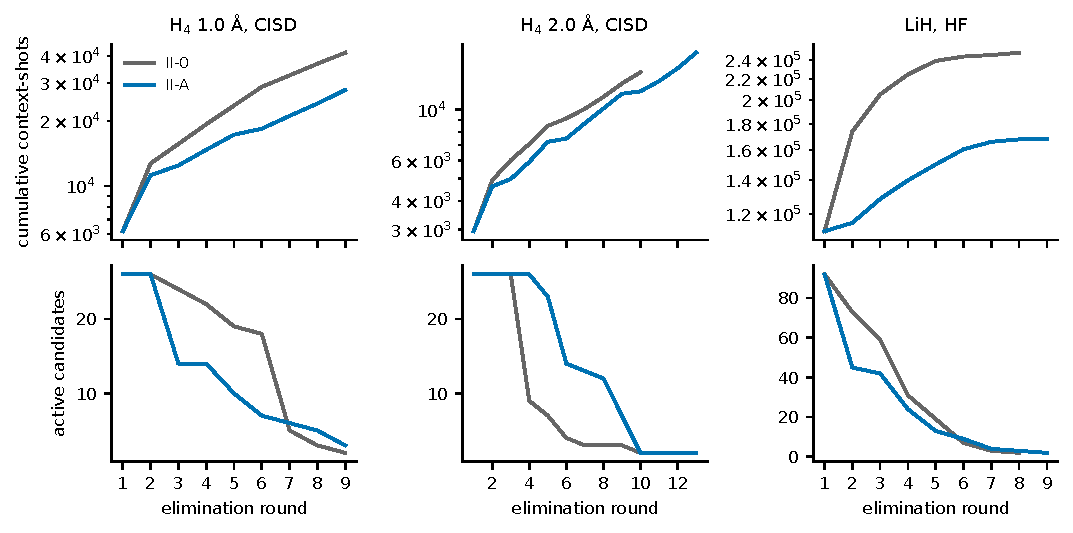
\includegraphics[width=\columnwidth]{figures/fig_rounds}
\caption{One selection with fixed (II-0) and learned (II-A) coefficients on the same random stream: cumulative context-shots (top) and active candidates (bottom) by elimination round, for three states.}
\label{fig:rounds}
\end{figure}

\subsection{Q6: Does the saving persist along a full ADAPT trajectory? Yes}

\begin{table}[!htb]
\centering\small
\caption{Measured ADAPT on H$_4$ side 1.0~\AA\ (STO-3G, UCCSD pool, $\delta=0.05$), 48 trajectories per method, $\rho=0.1$, empirical mode. Step $k$ selects at $\lvert\psi_k\rangle$; $\Delta E$ is the exact energy error after the selected generator is added and the parameters are reoptimized. Shots: median cumulative selection context-shots.}
\label{tab:q6}
\fitcol{%
\begin{tabular}{rrrrrrr}
\toprule
$k$ & $\max_i\lvert g_i\rvert$ & rel.\ gap & $\Delta E$ (mHa) & II-0 & II-A & II-E \\
\midrule
0 & 0.295 & 7.3\% & 137.6 & $7.8\times10^{4}$ & $5.4\times10^{4}$ & $5.8\times10^{4}$ \\
1 & 0.274 & 3.0\% & 120.4 & $1.8\times10^{5}$ & $1.2\times10^{5}$ & $1.3\times10^{5}$ \\
2 & 0.261 & tie & 106.2 & $2.7\times10^{5}$ & $1.6\times10^{5}$ & $1.9\times10^{5}$ \\
3 & 0.269 & 32.6\% & 91.1 & $2.9\times10^{5}$ & $1.8\times10^{5}$ & $2.0\times10^{5}$ \\
4 & 0.148 & tie & 85.8 & $8.1\times10^{5}$ & $4.8\times10^{5}$ & $4.1\times10^{5}$ \\
5 & 0.164 & 14.7\% & 79.1 & $9.7\times10^{5}$ & $5.7\times10^{5}$ & $4.8\times10^{5}$ \\
6 & 0.139 & 0.8\% & 16.4 & $1.19\times10^{6}$ & $7.7\times10^{5}$ & $6.8\times10^{5}$ \\
7 & 0.262 & 67.9\% & 8.4 & $1.21\times10^{6}$ & $7.8\times10^{5}$ & $7.0\times10^{5}$ \\
8 & 0.084 & tie & 5.4 & $1.82\times10^{6}$ & $1.06\times10^{6}$ & $1.06\times10^{6}$ \\
9 & 0.099 & 93.4\% & 1.1 & $1.88\times10^{6}$ & $1.11\times10^{6}$ & $1.09\times10^{6}$ \\
\bottomrule
\end{tabular}}
\end{table}

Yes. On H$_4$ the learned designs lower the cumulative selection cost to chemical accuracy by $41$--$42\%$ (Table~\ref{tab:q6}), and by $41$--$44\%$ on the stretched geometry (median $1.59\times10^7$ for II-0, $9.39\times10^6$ for II-A, $8.85\times10^6$ for II-E). Selections made from shot-limited data barely altered the trajectory. All 288 H$_4$ trajectories took the same number of steps as exact ADAPT and ended at the same energy. 90--94\% of their selections were the exact best generator (ties included), 90--96\% were 1~mHa-good, every one was $\rho$-good, and the mean shortfall of the selected gradient was 0.13--0.20\%. Chemical accuracy is reached after 10 steps (1.09~mHa) on H$_4$ 1.0 and after 6 steps (0.68~mHa) on LiH. There the learned designs lower the median selection cost from $8.6\times10^7$ (II-0) to $4.9\times10^7$ (II-A, $-42\%$) and $3.4\times10^7$ (II-E, $-60\%$), with 94--96\% exact-best and 96--97\% 1~mHa-good selections over 30 trajectories per method. One of 181 selections per learned method was not $\rho$-good (shortfall 13--15\%). In each learned method that trajectory took one extra step and ended $0.03$~mHa lower in energy error ($0.66$ against $0.68$~mHa). On the stretched geometry the pool itself stalls 3.22~mHa above FCI. The cost concentrates at the tied and small-gap steps: the three tied steps take 56--61\% of the median total on H$_4$ 1.0, and on the stretched geometry the tied step 8 ($\max_i\lvert g_i\rvert=0.0094$) alone takes 85--87\%. Without $\rho$-good stopping these steps do not terminate; exact identification on the tied step 4 ran to $1.7\times10^9$ shots in a single trial.

\begin{figure*}[!htb]
\centering
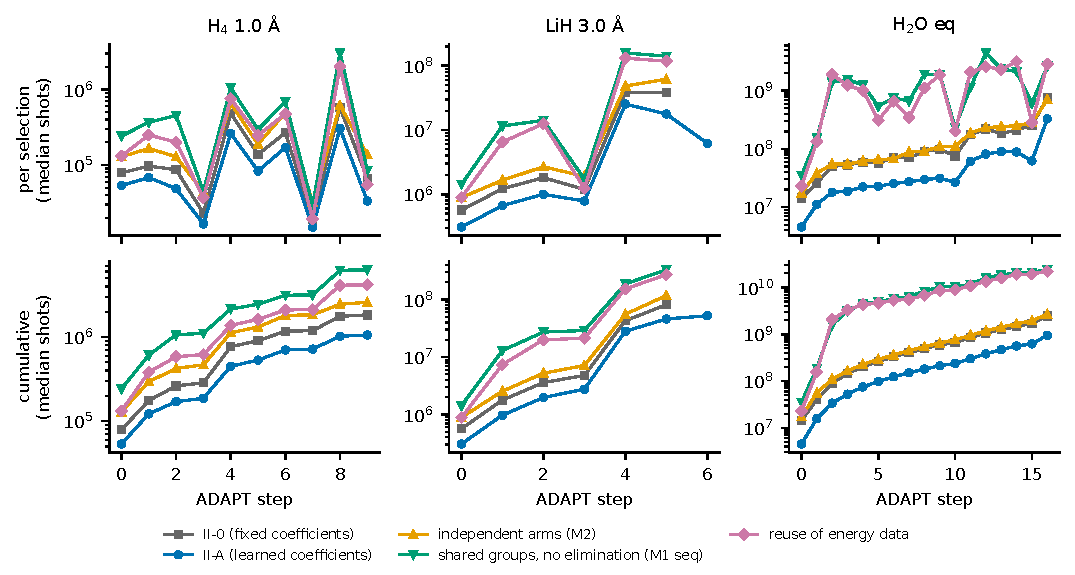
\includegraphics[width=\textwidth]{figures/fig_trajectory}
\caption{Measured ADAPT trajectories: median shots of each selection (top) and cumulative (bottom) for II-0, II-A, independent elimination (M2), the sequential all-gradient estimator (M1 seq) and the reuse baseline, on H$_4$ at 1.0~\AA, LiH at 3.0~\AA\ and H$_2$O at equilibrium.}
\label{fig:trajectory}
\end{figure*}

\subsection{Q7: Is selection still the bottleneck? Not once it is compressed}

\begin{table}[!htb]
\centering\small
\caption{Measurement cost of complete ADAPT runs (STO-3G, UCCSD pool, measured trajectories to chemical accuracy). $C_{\mathrm{sel}}$: static all-gradient estimation (M1 at its best, planning bound at radius $\rho\max_i\lvert g_i\rvert/2$), II-0 and II-A (measured medians); $C_{\mathrm{opt}}$: cost model of Sec.~\ref{sec:resources} with $\eta=2$ and $\eta=4$. Share: $C_{\mathrm{sel}}/C_{\mathrm{ADAPT}}$ at $\eta=2$. $S_{\mathrm{total}}$: Eq.~\eqref{eq:stotal} from M1 to the best measured method (II-E on LiH), at $\eta=2$ / $\eta=4$. Ranges: two independent builds of the Hamiltonian, whose SCF solutions differ within degenerate orbitals, which changes the Pauli expansion of $\hat H$ and the optimizer's evaluation counts.}
\label{tab:q7}
\footnotesize\setlength{\tabcolsep}{3.5pt}
\fitcol{%
\begin{tabular}{lrrrrr}
\toprule
 & \multicolumn{3}{c}{$C_{\mathrm{sel}}$} & \multicolumn{2}{c}{$C_{\mathrm{opt}}$} \\
\cmidrule(lr){2-4}\cmidrule(lr){5-6}
Geometry & M1 & II-0 & II-A & $\eta=2$ & $\eta=4$ \\
\midrule
H$_4$ 1.0 & $4.1\times10^{7}$ & $1.9\times10^{6}$ & $1.1\times10^{6}$ & $1.6$--$2.1\times10^{9}$ & $3.1$--$4.1\times10^{9}$ \\
H$_4$ 2.0 & $2.8\times10^{8}$ & $1.6\times10^{7}$ & $9.4\times10^{6}$ & $2.4$--$2.8\times10^{9}$ & $4.5$--$5.4\times10^{9}$ \\
LiH & $5.6\times10^{9}$ & $8.6\times10^{7}$ & $4.9\times10^{7}$ & $6.7\times10^{8}$ & $1.3\times10^{9}$ \\
\midrule
Geometry & \multicolumn{3}{r}{share, M1 / II-0 / II-A} & \multicolumn{2}{r}{$S_{\mathrm{total}}$} \\
\midrule
H$_4$ 1.0 & \multicolumn{3}{r}{1.9--2.5 / 0.09--0.12 / 0.05--0.07\%} & \multicolumn{2}{r}{1.02--1.03 / 1.01} \\
H$_4$ 2.0 & \multicolumn{3}{r}{9.1--10.5 / 0.57--0.67 / 0.34--0.40\%} & \multicolumn{2}{r}{1.10--1.11 / 1.05--1.06} \\
LiH & \multicolumn{3}{r}{89 / 11 / 6.9\% (II-E 4.8\%)} & \multicolumn{2}{r}{8.9--9.0 / 5.3} \\
\bottomrule
\end{tabular}}
\end{table}

It depends on the system, and once selection is compressed, optimization dominates (Table~\ref{tab:q7}). With static all-gradient estimation, selection is 1--11\% of the total measurement cost on H$_4$ but 82--89\% on LiH (for $\eta=2$ to $4$), whose 92-generator pool includes expensive generators with vanishing gradients. Shared BAI (II-0) makes selection 17--66 times cheaper, and the learned designs 30--37 times on H$_4$ and 114--166 times on LiH. Afterwards selection is below 0.7\% of the total on H$_4$ (below 0.4\% with the learned designs), 6--11\% on LiH with II-0, and 3--7\% with the learned designs. The end-to-end speedup is therefore large only where selection dominated: $S_{\mathrm{total}}=5.3$--$9.0$ on LiH, against $1.01$--$1.11$ on H$_4$. Beyond shared BAI, the learned designs change the total by 3--7\% on LiH and by less than 0.5\% on H$_4$. In all three systems the remaining bottleneck is the repeated reoptimization, whose cost grows with the number of parameters. This conclusion holds even though the cost model, with exact evaluation counts and no shot reuse, likely underestimates $C_{\mathrm{opt}}$. The comparison against M1 is conservative in M1's favor, because M1 is handed the exact gradient scale.

\paragraph{Sensitivity to the optimization cost.} The modeled $C_{\mathrm{opt}}$ is not the best the literature offers: Hessian recycling, for example, reports a reduction of the total measurement cost of ADAPT-VQE by about an order of magnitude for the 12- and 14-qubit molecules it studies~\cite{ramoa2025hessian}. Dividing $C_{\mathrm{opt}}$ by a factor $a$ and keeping the measured $C_{\mathrm{sel}}$ leaves the conclusion for H$_4$ unchanged: at $a=10$ selection is $1\%$ of the total at 1.0~\AA\ and $3$--$5\%$ at 2.0~\AA. For LiH it changes. At $a=10$ selection is $56\%$ of the total with II-0, $42\%$ with II-A and $34\%$ with II-E, and it equals the optimization cost at $a^\star=C_{\mathrm{opt}}/C_{\mathrm{sel}}=7.8$, $13.6$ and $19.7$. On LiH the learned designs then shorten the total by a further factor of $1.31$ (II-A) and $1.51$ (II-E) relative to II-0, instead of the $3$--$7\%$ above. The statement that reoptimization dominates is therefore a statement about the optimizer of the cost model and about the system: it holds on H$_4$ for any $a$ up to about 170, and on LiH only for $a\lesssim8$.

\subsection{Q8: How does the method compare with published baselines? Fewer shots than the strongest, which depends on the pool}
\label{sec:q8}

Q1--Q7 compared the method with reference strategies that we defined. Q8 asks whether the saving survives against the strategies of the published work, so that the answer does not depend on our choice of reference. Every baseline of Sec.~\ref{sec:external} is run from sampled outcomes under the rules of this work (radii, confidence rule, stopping rule and first radius) and with the optimal shot allocation, so the ratios below compare estimation strategies, not accounting conventions or heuristic schedules. Each baseline isolates one idea. The sequential M1 estimates all gradients on the shared fully commuting contexts, with the covariances of the shared estimates, but eliminates nothing. Independent BAI (M2, with Successive Elimination~\cite{evendar2006,huang2026} or with our pairwise rule) eliminates but shares nothing. The static M1 is handed the exact gap and variances. The reuse baseline~\cite{ikhtiarudin2025} starts from the shots of the last energy evaluation, and informationally complete measurements~\cite{nykanen2025} produce all gradients from one data set of another kind. If a published strategy were cheaper on some state, the saving of Q1--Q7 would be an artifact of our references; if the strongest baseline changed with the state, the value of sharing and of elimination would depend on it. The systems are those of Q1--Q7 and the stretched and ADAPT states of H$_2$O, which have the largest UCCSD pool, and the pools of the ADAPT literature test whether the saving depends on the structure of the UCCSD gradients. All results are simulations with shots drawn from the exact outcome distribution of the noiseless state.

As a check of the implementations, the sampled M1 static reproduces its planning bound: it costs $59{,}671$ shots on H$_4$ at 1.0~\AA\ (CISD) against $59{,}642$ for the bound and $3{,}564{,}398$ on LiH against $3{,}563{,}904$, and along the measured trajectories $4.137\times10^{7}$ (H$_4$) and $5.631\times10^{9}$ (LiH) shots, against $4.137\times10^{7}$ and $5.637\times10^{9}$ in Q7. Sampled independent BAI brackets its planning bound on H$_2$O at equilibrium (CISD): $3.7\times10^{10}$ shots with the pairwise rule and $6.6\times10^{10}$ with Successive Elimination, against $4.65\times10^{10}$.

% BEGIN GENERATED sota_tables
\begin{table*}[!htb]
\centering\small
\caption{The strongest baseline against our methods, per state (mean context-shots; ratios of the baseline's cost to ours, so a value above one is a win). STO-3G, UCCSD pool, $\delta=0.05$; 100 to 200 trials per state and 12 to 48 trajectories per method. Without free data: the best of M1 static, M1 seq and M2 against II-0 and II-A. With the energy data of the last VQE evaluation (1~mHa): the best of all baselines including the reuse baseline against the better of II-0 + reuse and II-A + reuse. Rows marked sign-aware use the sign-aware rule throughout. Rows whose selections were correct in fewer than 95\% of the trials are excluded.}
\label{tab:q8best}
\footnotesize\setlength{\tabcolsep}{3.5pt}
\begin{tabular}{lllrrrlrr}
\toprule
state & rule & best baseline & cost & II-0 & II-A & best, with data & cost & ours + data \\
\midrule
H$_4$ 1.0 CISD & pairwise & M1 seq & 55\,870 & 1.35 & 2.06 & reuse FC & 33\,988 & 2.40 \\
H$_4$ 1.0 CISD & sign-aware & M1 seq & 53\,260 & 1.13 & 1.59 & reuse FC & 36\,824 & 1.74 \\
H$_4$ 2.0 CISD & pairwise & M1 seq & 41\,979 & 1.70 & 3.06 & reuse FC & 33\,638 & 3.14 \\
H$_4$ 2.0 CISD & sign-aware & M1 seq & 45\,085 & 1.73 & 2.35 & reuse FC & 36\,316 & 2.15 \\
LiH HF & pairwise & M1 seq & $8.33\times10^{5}$ & 2.73 & 4.52 & reuse FC & $4.10\times10^{5}$ & 2.36 \\
LiH HF & sign-aware & M2 sign-aware & $1.01\times10^{6}$ & 1.83 & 3.10 & M2 sign-aware & $1.01\times10^{6}$ & 3.11 \\
LiH ADAPT$_3$ & pairwise & M1 seq & $1.29\times10^{6}$ & 1.82 & 3.00 & reuse FC & $8.70\times10^{5}$ & 2.30 \\
LiH ADAPT$_3$ & sign-aware & M1 seq & $1.80\times10^{6}$ & 1.58 & 2.13 & reuse FC & $1.30\times10^{6}$ & 1.71 \\
LiH ADAPT$_5$ & pairwise & M2 pairw. & $9.41\times10^{7}$ & 1.43 & 2.17 & M2 pairw. & $9.41\times10^{7}$ & 3.16 \\
LiH ADAPT$_5$ & sign-aware & M2 sign-aware & $9.41\times10^{7}$ & 1.36 & 2.39 & M2 sign-aware & $9.41\times10^{7}$ & 3.34 \\
H$_2$O eq CISD & pairwise & M2 pairw. & $3.70\times10^{10}$ & 1.80 & 4.21 & M2 pairw. & $3.70\times10^{10}$ & 5.17 \\
H$_2$O eq CISD & sign-aware & M2 sign-aware & $3.70\times10^{10}$ & 1.80 & 4.21 & M2 sign-aware & $3.70\times10^{10}$ & 5.17 \\
H$_2$O str CISD & pairwise & M2 pairw. & $1.30\times10^{8}$ & 1.50 & 3.28 & M2 pairw. & $1.30\times10^{8}$ & 4.24 \\
H$_2$O str CISD & sign-aware & M2 sign-aware & $1.30\times10^{8}$ & 1.30 & 2.66 & M2 sign-aware & $1.30\times10^{8}$ & 3.21 \\
H$_2$O eq ADAPT$_{11}$ & pairwise & M2 pairw. & $2.33\times10^{8}$ & 1.21 & 2.86 & M2 pairw. & $2.33\times10^{8}$ & 3.68 \\
H$_2$O eq ADAPT$_{11}$ & sign-aware & M2 sign-aware & $2.33\times10^{8}$ & 1.16 & 3.06 & M2 sign-aware & $2.33\times10^{8}$ & 3.36 \\
H$_2$O str ADAPT$_8$ & pairwise & M2 pairw. & $2.64\times10^{8}$ & 1.44 & 3.08 & M2 pairw. & $2.64\times10^{8}$ & 3.96 \\
H$_2$O str ADAPT$_8$ & sign-aware & M2 sign-aware & $2.64\times10^{8}$ & 1.46 & 2.99 & M2 sign-aware & $2.64\times10^{8}$ & 3.84 \\
\midrule
H$_4$ 1.0 trajectory & sign-aware & M2 sign-aware & $2.67\times10^{6}$ & 1.42 & 2.41 & M2 sign-aware & $2.67\times10^{6}$ & 5.71 \\
H$_4$ 2.0 trajectory & sign-aware & M2 sign-aware & $2.31\times10^{7}$ & 1.45 & 2.47 & M2 sign-aware & $2.31\times10^{7}$ & 2.88 \\
LiH trajectory & sign-aware & M2 sign-aware & $1.21\times10^{8}$ & 1.41 & 2.44 & M2 sign-aware & $1.21\times10^{8}$ & 3.86 \\
H$_2$O eq trajectory & sign-aware & M2 sign-aware & $2.73\times10^{9}$ & 1.11 & 2.44 & M2 sign-aware & $2.73\times10^{9}$ & 3.07 \\
H$_2$O str trajectory & sign-aware & M2 sign-aware & $8.45\times10^{9}$ & 1.08 & 2.85 & M2 sign-aware & $8.45\times10^{9}$ & 3.56 \\
\bottomrule
\end{tabular}
\end{table*}

\begin{table*}[!htb]
\centering\small
\caption{Fixed states, sampled outcomes, covariances and radii estimated from the shots (exact identification, starting radius $\max_i\lvert g_i\rvert$): mean context-shots and, in brackets, the ratio to II-0. STO-3G, UCCSD pool, $\delta=0.05$; 200 trials on H$_4$, 100 to 200 on LiH, 100 on H$_2$O. M1 static is handed the exact gap and variances. The ``reuse'' rows hold the shots of one energy evaluation to 1~mHa for free (they are part of $C_{\mathrm{opt}}$) and charge only new shots. In square brackets, the percentage of correct selections when it is below 100\%.}
\label{tab:q8fixed}
\footnotesize\setlength{\tabcolsep}{2.4pt}
\begin{tabular}{lrrrrr}
\toprule
Method & H$_4$ 1.0 CISD & H$_4$ 2.0 CISD & LiH HF & H$_2$O eq CISD & H$_2$O str CISD \\
\midrule
\multicolumn{6}{l}{\emph{external baselines}} \\
M1 static & 59\,671 (1.44) & 58\,094 (2.35) & $3.56\times10^{6}$ (11.69) & $4.12\times10^{11}$ (20.06) & $5.72\times10^{9}$ (66.24) \\
M1 seq (no elimination) & 55\,870 (1.35) & 41\,979 (1.70) & $8.33\times10^{5}$ (2.73) & $9.42\times10^{10}$ (4.59) & $1.49\times10^{9}$ (17.25) \\
M2, Successive Elimination & $1.51\times10^{5}$ (3.63) & $1.41\times10^{5}$ (5.72) & $1.67\times10^{6}$ (5.47) & $6.58\times10^{10}$ (3.21) & $2.32\times10^{8}$ (2.68) \\
M2, pairwise rule & $1.01\times10^{5}$ (2.44) & $1.06\times10^{5}$ (4.28) & $1.01\times10^{6}$ (3.30) & $3.70\times10^{10}$ (1.80) & $1.30\times10^{8}$ (1.50) \\
\multicolumn{6}{l}{\emph{this work}} \\
II-0 (shared BAI) & 41\,463 (1.00) & 24\,699 (1.00) & $3.05\times10^{5}$ (1.00) & $2.05\times10^{10}$ (1.00) & $8.63\times10^{7}$ (1.00) \\
II-A (learned splitting) & 27\,129 (0.65) & 13\,727 (0.56) & $1.85\times10^{5}$ (0.60) & $8.80\times10^{9}$ (0.43) & $3.95\times10^{7}$ (0.46) \\
\multicolumn{6}{l}{\emph{with the energy data of the last VQE evaluation (FC)}} \\
shot reuse of Ikhtiarudin \textit{et al.} & 33\,988 (0.82) & 33\,638 (1.36) & $4.10\times10^{5}$ (1.34) & $1.83\times10^{11}$ (8.94) & $5.39\times10^{8}$ (6.24) \\
II-0 + reuse & 23\,997 (0.58) & 17\,129 (0.69) & $1.96\times10^{5}$ (0.64) & $2.03\times10^{10}$ (0.99) & $6.19\times10^{7}$ (0.72) \\
II-A + reuse, forced assignment & 14\,149 (0.34) & 10\,872 (0.44) & $3.51\times10^{5}$ (1.15){\,\scriptsize[92\%]} & $7.16\times10^{9}$ (0.35) & $3.05\times10^{7}$ (0.35) \\
II-A + reuse, home start & 14\,317 (0.35) & 10\,720 (0.43) & $1.74\times10^{5}$ (0.57) & $1.09\times10^{10}$ (0.53){\,\scriptsize[99\%]} & $3.79\times10^{7}$ (0.44) \\
\multicolumn{6}{l}{\emph{sign-aware rule (ratios to II-0 safe)}} \\
M1 seq & 53\,260 (1.13) & 45\,085 (1.73) & $1.81\times10^{6}$ (3.30) & $9.42\times10^{10}$ (4.59) & $1.54\times10^{9}$ (15.46) \\
II-0 & 47\,037 (1.00) & 26\,126 (1.00) & $5.49\times10^{5}$ (1.00) & $2.05\times10^{10}$ (1.00) & $9.98\times10^{7}$ (1.00) \\
II-A & 33\,467 (0.71) & 19\,157 (0.73) & $3.25\times10^{5}$ (0.59) & $8.80\times10^{9}$ (0.43) & $4.87\times10^{7}$ (0.49) \\
shot reuse of Ikhtiarudin \textit{et al.} & 36\,824 (0.78) & 36\,316 (1.39) & $1.07\times10^{6}$ (1.95) & $1.83\times10^{11}$ (8.94) & $6.02\times10^{8}$ (6.03) \\
II-0 + reuse & 27\,778 (0.59) & 20\,747 (0.79) & $4.12\times10^{5}$ (0.75) & $2.03\times10^{10}$ (0.99) & $7.20\times10^{7}$ (0.72) \\
II-A + reuse, forced assignment & 27\,689 (0.59) & 18\,891 (0.72) & $4.44\times10^{5}$ (0.81) & $7.16\times10^{9}$ (0.35) & $4.04\times10^{7}$ (0.40) \\
II-A + reuse, home start & 21\,197 (0.45) & 16\,925 (0.65) & $3.24\times10^{5}$ (0.59) & $1.13\times10^{10}$ (0.55) & $4.81\times10^{7}$ (0.48) \\
\bottomrule
\end{tabular}
\end{table*}

\begin{table*}[!htb]
\centering\small
\caption{Measured ADAPT trajectories to chemical accuracy ($\rho=0.1$, a-priori starting radius, sign-aware rule): median cumulative selection context-shots and, in brackets, the ratio to II-0. STO-3G, UCCSD pool, $\delta=0.05$; 48 trajectories per method on H$_4$, 30 on LiH, 12 on H$_2$O. M1 static uses the exact gradient scale and variances. A dash means that the configuration was not run.}
\label{tab:q8traj}
\footnotesize\setlength{\tabcolsep}{4pt}
\begin{tabular}{lrrrrr}
\toprule
Method & H$_4$ 1.0 & H$_4$ 2.0 & LiH & H$_2$O eq & H$_2$O str \\
\midrule
\multicolumn{6}{l}{\emph{external baselines}} \\
M1 static & $4.14\times10^{7}$ (22.04) & $2.77\times10^{8}$ (17.41) & $5.63\times10^{9}$ (65.70) & $2.44\times10^{11}$ (98.95) & $9.55\times10^{11}$ (121.61) \\
M1 seq & $5.74\times10^{6}$ (3.06) & $3.81\times10^{7}$ (2.39) & $3.47\times10^{8}$ (4.05) & $2.43\times10^{10}$ (9.85) & $8.39\times10^{10}$ (10.68) \\
M2, Successive Elimination & $3.18\times10^{6}$ (1.69) & $3.49\times10^{7}$ (2.19) & $2.17\times10^{8}$ (2.53) & $5.25\times10^{9}$ (2.13) & $1.73\times10^{10}$ (2.20) \\
M2, sign-aware & $2.67\times10^{6}$ (1.42) & $2.31\times10^{7}$ (1.45) & $1.21\times10^{8}$ (1.41) & $2.73\times10^{9}$ (1.11) & $8.45\times10^{9}$ (1.08) \\
\multicolumn{6}{l}{\emph{this work}} \\
II-0 & $1.88\times10^{6}$ (1.00) & $1.59\times10^{7}$ (1.00) & $8.57\times10^{7}$ (1.00) & $2.46\times10^{9}$ (1.00) & $7.85\times10^{9}$ (1.00) \\
II-A & $1.11\times10^{6}$ (0.59) & $9.39\times10^{6}$ (0.59) & $4.94\times10^{7}$ (0.58) & $1.12\times10^{9}$ (0.46) & $2.97\times10^{9}$ (0.38) \\
II-E & $1.09\times10^{6}$ (0.58) & $8.85\times10^{6}$ (0.56) & $3.41\times10^{7}$ (0.40) & -- & -- \\
\multicolumn{6}{l}{\emph{with the energy data of the last VQE evaluation (FC)}} \\
shot reuse of Ikhtiarudin \textit{et al.} & $4.23\times10^{6}$ (2.25) & $3.70\times10^{7}$ (2.32) & $2.79\times10^{8}$ (3.26) & $2.24\times10^{10}$ (9.10) & $6.87\times10^{10}$ (8.75) \\
II-0 + reuse & $1.03\times10^{6}$ (0.55) & $1.31\times10^{7}$ (0.82) & $3.94\times10^{7}$ (0.46) & $2.18\times10^{9}$ (0.89) & $6.17\times10^{9}$ (0.79) \\
II-A + reuse & $4.67\times10^{5}$ (0.25) & $8.04\times10^{6}$ (0.50) & $3.13\times10^{7}$ (0.37) & $8.91\times10^{8}$ (0.36) & $2.37\times10^{9}$ (0.30) \\
\bottomrule
\end{tabular}
\end{table*}

\begin{table*}[!htb]
\centering\small
\caption{Operator pools (CISD and HF states of H$_4$ at 1.0~\AA, HF state of LiH; STO-3G, $\delta=0.05$, 100 trials per row). $K$: generators; $\lvert\mathcal B_0\rvert$: parent support; $N$: parent FC contexts; uses: gradients per Pauli product. Planning bounds (exact gradients and variances) are given as ratios M1/M3 and M2/M3 where the leader is unique; qubit-type pools have exactly tied leaders. Right: sampled outcomes with estimated variances and a $\rho=0.1$ stop, mean context-shots; a dash: no planning bound, because the leaders are tied.}
\label{tab:q8pools}
\footnotesize\setlength{\tabcolsep}{3pt}
\begin{tabular}{llrrrrrrrrrr}
\toprule
state & pool & $K$ & $\lvert\mathcal B_0\rvert$ & $N$ & uses & M1/M3 & M2/M3 & II-0 & II-A & M1 seq & M2 pairw. \\
\midrule
H$_4$ 1.0 CISD & UCCSD & 26 & 1\,276 & 53 & 3.25 & 1.20 & 2.07 & 37\,974 & 25\,347 & 48\,245 & 99\,383 \\
H$_4$ 1.0 CISD & QEB & 26 & 2\,036 & 65 & 2.04 & 1.26 & 2.15 & 37\,404 & 25\,163 & 44\,077 & 93\,253 \\
H$_4$ 1.0 CISD & qubit-ADAPT & 160 & 2\,064 & 65 & 3.65 & -- & -- & $4.45\times10^{6}$ & $2.97\times10^{6}$ & $1.08\times10^{7}$ & $1.59\times10^{7}$ \\
H$_4$ 1.0 CISD & generalized QEB & 90 & 3\,332 & 80 & 5.21 & 1.29 & 3.34 & 53\,312 & 31\,035 & 65\,102 & $3.04\times10^{5}$ \\
H$_4$ 1.0 CISD & generalized qubit & 328 & 3\,344 & 80 & 4.66 & -- & -- & $7.82\times10^{6}$ & $8.45\times10^{5}$ & $1.88\times10^{7}$ & $2.22\times10^{7}$ \\
H$_4$ 1.0 CISD & OVP-CEO & 96 & 3\,332 & 80 & 3.40 & -- & -- & $2.23\times10^{5}$ & $1.24\times10^{5}$ & $2.11\times10^{5}$ & $1.37\times10^{6}$ \\
\midrule
H$_4$ 1.0 HF & UCCSD & 26 & 1\,276 & 53 & 3.25 & 3.95 & 1.50 & 77\,771 & 45\,236 & $2.50\times10^{5}$ & $1.42\times10^{5}$ \\
H$_4$ 1.0 HF & QEB & 26 & 2\,036 & 65 & 2.04 & 3.30 & 1.56 & 73\,018 & 34\,199 & $1.98\times10^{5}$ & $1.55\times10^{5}$ \\
H$_4$ 1.0 HF & qubit-ADAPT & 160 & 2\,064 & 65 & 3.65 & -- & -- & $2.56\times10^{6}$ & $2.14\times10^{5}$ & $3.62\times10^{6}$ & $5.31\times10^{6}$ \\
H$_4$ 1.0 HF & generalized QEB & 90 & 3\,332 & 80 & 5.21 & 3.90 & 1.90 & 78\,665 & 46\,989 & $2.18\times10^{5}$ & $2.23\times10^{5}$ \\
H$_4$ 1.0 HF & generalized qubit & 328 & 3\,344 & 80 & 4.66 & -- & -- & $2.35\times10^{6}$ & $5.58\times10^{5}$ & $5.71\times10^{6}$ & $6.93\times10^{6}$ \\
H$_4$ 1.0 HF & OVP-CEO & 96 & 3\,332 & 80 & 3.40 & -- & -- & 88\,532 & 51\,689 & $2.69\times10^{5}$ & $4.31\times10^{5}$ \\
\midrule
LiH HF & UCCSD & 92 & 30\,196 & 980 & 3.99 & 10.69 & 3.42 & $3.03\times10^{5}$ & $1.83\times10^{5}$ & $5.67\times10^{5}$ & $1.01\times10^{6}$ \\
LiH HF & QEB & 92 & 83\,512 & 1483 & 1.68 & 9.53 & 5.61 & $2.13\times10^{5}$ & $1.41\times10^{5}$ & $3.41\times10^{5}$ & $1.16\times10^{6}$ \\
LiH HF & qubit-ADAPT & 640 & 83\,964 & 1482 & 2.27 & -- & -- & $5.48\times10^{6}$ & $1.14\times10^{6}$ & $9.71\times10^{7}$ & $2.22\times10^{7}$ \\
LiH HF & generalized QEB & 570 & $2.25\times10^{5}$ & 2004 & 4.36 & 10.34 & 8.02 & $2.20\times10^{5}$ & $1.38\times10^{5}$ & $3.26\times10^{5}$ & $4.50\times10^{6}$ \\
LiH HF & generalized qubit & 2100 & $2.25\times10^{5}$ & 2004 & 2.80 & -- & -- & $8.26\times10^{6}$ & $1.83\times10^{6}$ & $8.52\times10^{7}$ & $6.95\times10^{7}$ \\
LiH HF & OVP-CEO & 660 & $2.25\times10^{5}$ & 2004 & 2.87 & -- & -- & $4.67\times10^{5}$ & $2.70\times10^{5}$ & $3.82\times10^{6}$ & $6.49\times10^{6}$ \\
\bottomrule
\end{tabular}
\end{table*}

\begin{table}[!htb]
\centering\small
\caption{Reuse of the energy measurement against the standard error $\varepsilon_E$ of the last energy evaluation (H$_4$ 1.0~\AA, CISD; mean context-shots, 100 trials, 200 at 1~mHa). The data held for free scale as $\varepsilon_E^{-2}$. Last row: the same methods without free data.}
\label{tab:q8eps}
\footnotesize\setlength{\tabcolsep}{2.2pt}
\begin{tabular}{rrrrr}
\toprule
$\varepsilon_E$ (mHa) & free shots & Ikhtiarudin FC & II-0 + reuse & II-A + reuse \\
\midrule
0.3 & $5.79\times10^{6}$ & 33\,535 & 24\,245 & 13\,402 \\
1 & $5.21\times10^{5}$ & 33\,988 & 23\,997 & 14\,149 \\
3 & 57\,891 & 37\,228 & 26\,387 & 18\,740 \\
10 & 5\,211 & 47\,033 & 38\,053 & 25\,338 \\
30 & 580 & 53\,460 & 39\,116 & 28\,181 \\
\midrule
none & 0 & 55\,870 & 41\,463 & 27\,129 \\
\bottomrule
\end{tabular}
\end{table}
% END GENERATED sota_tables

\paragraph{The strongest baseline depends on the state.} The learned designs need fewer shots than the strongest baseline in every row of Table~\ref{tab:q8best}; Table~\ref{tab:q8fixed} gives all methods on five of the fixed states. Without free data, II-A needs $2.1$ to $4.5$ times fewer shots than the strongest of the sequential M1 and independent BAI (with Successive Elimination or the pairwise rule) on the 9 fixed states, $1.6$ to $4.2$ times fewer with the sign-aware rule, and $2.4$ to $2.8$ times fewer along the five measured trajectories. Shared elimination with fixed estimators (II-0) wins by less: $1.2$ to $2.7$, $1.1$ to $1.8$ and $1.1$ to $1.5$ times. With the pairwise rule the strongest baseline is the sequential M1 on the two H$_4$ states and on LiH at the Hartree--Fock state and after three steps, and independent BAI on LiH after five steps and on all four H$_2$O states. Each of them lacks one ingredient of II-0, and it is the smaller one. On the first four states sharing is worth more than elimination (II-0 against independent BAI: $2.4$ to $4.3$ times; against the sequential M1: $1.3$ to $2.7$ times), and on the other five elimination is worth more ($4.6$ to $27.8$ times against $1.2$ to $1.8$). This is the balance seen with exact variances in Q2: sharing wins where the gap is wide compared with the spread of the gradients, and elimination where many generators of large variance have small gradients. We did not test whether it accounts for the switch on LiH between three and five steps. The static M1 is never the strongest. It costs $1.1$ to $5.8$ times the sequential M1 on the fixed states and $7.2$ to $16$ times along the trajectories.

\paragraph{Free energy data.} The reuse baseline starts from the shots of the last energy evaluation, which belong to $C_{\mathrm{opt}}$ and cost the selection nothing. One evaluation to 1~mHa holds more shots than a selection needs on the small systems ($5.2\times10^{5}$ on H$_4$ at 1.0~\AA\ against $4.1\times10^{4}$ for II-0, and $5.6\times10^{5}$ on LiH) and far fewer on H$_2$O ($7.3\times10^{6}$ and $9.1\times10^{6}$ at the two geometries, against $2.05\times10^{10}$ and $8.6\times10^{7}$ for II-0). The data cover only part of what a selection needs. The Pauli products measured by the groups of $\hat H$ are $11\%$ of the support of the gradients on H$_4$ ($22\%$ of the coefficient mass) and $15\%$ ($34\%$) on LiH for fully commuting groups, and $23\%$ ($25\%$) and $13\%$ ($31\%$) for the QWC cliques of the original, which are measured in a product basis. With the pairwise rule, reading these products from the data lowers the cost of the sequential M1 by $20$ to $39\%$ on H$_4$ and by $20$ to $51\%$ on LiH, that of II-0 by $31$ to $42\%$ and $36$ to $38\%$, and that of II-A, started from the home design, by $22$ to $47\%$ and $6$ to $32\%$. With the sign-aware rule the reductions are $19$ to $31\%$ and $9$ to $41\%$ for the sequential M1, $21$ to $41\%$ and $25$ to $41\%$ for II-0, and $12$ to $37\%$ and $0$ to $29\%$ for II-A. The data help the new methods about as much as the baseline, so the ranking does not change: with the data, the better of II-0 and II-A needs $1.7$ to $5.2$ times fewer shots than the best baseline with the data on the 18 fixed-state rows of Table~\ref{tab:q8best}, and $2.9$ to $5.7$ times fewer along the trajectories. The benefit is a statement about the precision of the energy evaluation (Table~\ref{tab:q8eps}): it saturates below 1~mHa, where the cost is set by the products that the energy groups do not cover, and has vanished at 30~mHa. QWC cliques cost more than the fully commuting groups, without the data ($113{,}209$ against $55{,}870$ shots on H$_4$, $2.0$ times) and with it ($67{,}205$ against $33{,}988$). They cover about as much of the coefficient mass, so the cost is set by the grouping of the rest, which is twice as expensive.

\paragraph{Where the free data do not explain the effect.} On H$_2$O the data are small compared with what a selection needs ($7.3\times10^{6}$ and $9.1\times10^{6}$ shots against $9.4\times10^{10}$ and $1.5\times10^{9}$ for the sequential M1 on the CISD states, Table~\ref{tab:q8fixed}), yet the reuse baseline changes the cost of the sequential M1 by $+95\%$, $+21\%$ and $+11\%$ on three of the four states and by $-64\%$ on the fourth (stretched CISD; pairwise rule, and $+95\%$, $+18\%$, $+11\%$ and $-61\%$ with the sign-aware rule). Since the data are small, the change is not due to them. We attribute it to the forced reassignment of every product to an energy context that measures it, which we expect to split the fragments of the parent contexts, but we have not isolated this. The same reassignment lowers the cost of II-A on H$_2$O by $19$ to $23\%$ with the pairwise rule, whereas from the home design the cost changes by $-6$ to $+24\%$. On LiH at the Hartree--Fock state the forced assignment makes II-A cost $90\%$ more, and the pairwise rule then selects a wrong generator in $7.5\%$ of the trials (the plug-in-sign failure of Q3); with the sign-aware rule it costs $37\%$ more and every selection is correct. Letting the learned splitting decide whether to use the energy contexts, as the home start does, removes this loss on H$_4$ and LiH without ever raising the cost (the extra contexts alone leave it unchanged: $33{,}483$ against $33{,}467$ shots on H$_4$ at 1.0~\AA\ with the sign-aware rule). The columns ``ours + data'' of Table~\ref{tab:q8best} use the best of the three variants per state, as the baseline gets the better of its fully commuting and QWC versions.

\paragraph{Sign-aware rule.} The pairwise rule takes the signs of the estimates at face value and fails when they are wrong (Q3). Every row marked sign-aware was correct in every trial. The safeguard changes the cost of II-A by a factor between $0.9$ and $2.0$ (on LiH, $3.25\times10^{5}$ against $1.85\times10^{5}$ shots), and the baselines are run with the same rule, so the advantage of II-A over the strongest of them stays at $1.6$ to $4.2$ times.

\paragraph{Along ADAPT trajectories.} Table~\ref{tab:q8traj} repeats the comparison along complete runs, with the sign-aware rule and the a priori starting radius: 48 trajectories per method and geometry on H$_4$, 30 on LiH and 12 on each H$_2$O geometry. All of them take the number of steps of exact ADAPT ($10$ on both H$_4$ geometries, $6$ on LiH, $17$ and $18$ on H$_2$O), except one LiH trajectory per learned method (Q6), and all reach chemical accuracy except those on the stretched H$_4$ geometry, whose pool stalls at $3.2$~mHa. Independent BAI with the sign-aware rule is the strongest baseline on all five systems. This is the side of the balance that the states of small gradient take above, and it is consistent with Q6, where the cost concentrates at tied and small-gap steps. Independent BAI costs $1.1$ to $1.5$ times II-0, whereas the sequential M1 costs $3.1$, $2.4$ and $4.1$ times II-0 on H$_4$ (two geometries) and LiH and $9.9$ to $10.7$ times on H$_2$O, and the static M1 $17$ to $66$ times on H$_4$ and LiH (Q7) and $99$ and $122$ times on H$_2$O. With the energy data the learned designs are $2.9$ to $5.7$ times cheaper than independent BAI, and II-A with the data is $4.6$ to $29$ times cheaper than the reuse baseline. The largest factors are on H$_2$O ($25$ and $29$), where the reuse baseline costs about $9$ times II-0.

\paragraph{Other operator pools.} The structure that sharing exploits depends on the pool (Table~\ref{tab:q8pools}), so we repeat the comparison with the pools of the ADAPT literature (Sec.~\ref{sec:external}). With qubit excitations a Pauli product appears in fewer gradients ($2.0$ instead of $3.3$ per product on H$_4$, $1.7$ instead of $4.0$ on LiH) and the support is larger ($1{,}276\to2{,}036$ and $30{,}196\to83{,}512$ products), yet the planning gain of shared elimination survives. With the QEB pool M3 is $1.26$ and $2.15$ times cheaper than M1 and M2 on H$_4$ ($1.20$ and $2.07$ with UCCSD) and $9.5$ and $5.6$ times cheaper on LiH ($10.7$ and $3.4$ with UCCSD). The generalized QEB pool of LiH has $570$ generators, $225{,}369$ products and $4.4$ uses per product, and M3 is $10.3$ and $8.0$ times cheaper than M1 and M2. The qubit-ADAPT, generalized qubit and OVP-CEO pools have exactly tied leaders (spin and spatial partners), so exact planning bounds are undefined and only runs that stop at a $\rho$-good generator apply. At $\rho=0.1$ on sampled outcomes II-A is the cheapest method on all 12 combinations of pool and state on H$_4$ (the CISD and Hartree--Fock states at 1.0~\AA; $1.7$ to $22.2$ times cheaper than the better of the sequential M1 and independent BAI) and on all 6 pools of LiH ($2.4$ to $38.0$ times). II-0 alone is the cheapest in 11 of the 12 cases on H$_4$ ($0.9$ to $3.0$ times; it loses ($0.94$) to the sequential M1 on the OVP-CEO pool at the CISD state) and in all 6 on LiH ($1.5$ to $8.4$ times). The selection was $\rho$-good in at least $99\%$ of the trials of every row. The saving is largest on the qubit pools (up to $22$ times on H$_4$ and $38$ on LiH) and smallest on the OVP-CEO pool at the CISD state of H$_4$ ($1.7$ times) and on the excitation pools ($1.8$ to $4.6$ times). The pools differ in size and in the number of uses per product at the same time, so we cannot say which property controls the size of the saving.

\paragraph{Informationally complete measurements.} AIM-ADAPT-VQE~\cite{nykanen2025} measures every qubit with an informationally complete (IC) POVM and obtains the energy and all gradients from the same data. An IC shot measures all qubits in the POVM and is a different resource from a context-shot, so only statistical efficiency is compared. We simulate the data model exactly for the unoptimized tetrahedral (SIC) POVM, for which the single-shot second moment of a weight-$w$ Pauli product is $3^w$ and the leading gradient of H$_4$ at 1.0~\AA\ has a per-shot variance of $66$. The selection then needs a median of $3.12\times10^{6}$ IC shots (mean $4.00\times10^{6}$; $99.5\%$ correct in 200 trials with anytime intervals) at 1.0~\AA\ and $7.15\times10^{5}$ at 2.0~\AA, against $4.1\times10^{4}$ and $2.5\times10^{4}$ context-shots for II-0 and $2.7\times10^{4}$ and $1.4\times10^{4}$ for II-A. On LiH the median is $2.61\times10^{8}$ IC shots ($\rho=0.1$, oracle radii; one trial of 100 needed $10^{13}$ and dominates the mean), against $1.83\times10^{5}$ context-shots for II-A at the same $\rho$. The IC data of one energy evaluation to 1~mHa are $4.87\times10^{7}$ shots on H$_4$ and $5.71\times10^{8}$ on LiH, more than the selection needs, so the selection is free given those data: this is the ``no additional measurement overhead'' of AIM-ADAPT-VQE~\cite{nykanen2025}. The energy itself, however, takes about $93$ times (H$_4$) and $10^{3}$ times (LiH) the context-shots of fully commuting groups. Whether the selection is then cheaper than with II-A depends on the cost of an IC shot relative to a context-shot, which we do not model. IC single-shot estimators are also heavy tailed. Without the anytime correction, at least one normal interval missed the exact value in $69\%$ of $100$ trials on H$_4$ and the best candidate was eliminated in $3$ of them; the correction costs a factor of $2.3$ in the median. These numbers are an upper bound for the optimized scheme, whose POVM parameters are adapted to lower the variance of the energy.

\paragraph{Takeaway.} Against the strongest published baseline, run under the same rules, the learned designs need $1.6$ to $4.5$ times fewer shots on every fixed state, $2.4$ to $2.8$ times fewer along every trajectory and $1.7$ to $38$ times fewer on every operator pool, and shared elimination without learning is cheaper than every baseline except in one pool case. No single baseline is strongest everywhere. The sequential all-gradient estimator wins where sharing is worth more than elimination, and independent elimination where the reverse holds, so the saving does not come from a weak reference. Free energy data help the baselines and the new methods alike and do not change the ranking. These ratios start every fixed-state selection from the exact largest gradient; with an a priori first radius and the default minimum of 50 shots the learned designs lose on three late states, which a larger minimum repairs (Q9). These comparisons give every method fully commuting contexts of unrestricted depth and measure the baselines as we implemented them. What changes when the circuits are shallower, when the contexts are those of Anastasiou \textit{et al.}~\cite{anastasiou2023}, and when the radii are less conservative is the subject of the Discussion.


% BEGIN REFEREE RESULTS
\subsection{Q9: Do the savings survive an a priori start, a run-wide guarantee and uncertainty? Yes, once the minimum number of shots is raised}
\label{sec:q9}

Q1--Q8 start every selection from the exact largest gradient (to set the first radius) and use intervals that hold for each round. A reader may object to both, and also to the pairwise elimination rule that gave the headline numbers. This subsection repeats the comparison with the sign-aware rule, an a priori first radius (a bound computed from the Hamiltonian and the pool, with no exact gradient), and intervals that hold over the whole selection (anytime intervals: the confidence $\delta$ is divided over the rounds as $\delta_r=6\delta/(\pi^2r^2)$). It adds two states of LiH at 1.6~\AA\ (near its equilibrium bond length; exact ADAPT reaches chemical accuracy in five steps) and four states of linear BeH$_2$ (14 qubits, $K=204$; exact ADAPT needs ten steps), and reports bootstrap intervals (10{,}000 resamples of the trials, numerator and denominator resampled independently). Every row uses the sign-aware rule and an a priori start; shots are context-shots; the bracketed number in Table~\ref{tab:apriori} is the share of correct selections when it is below $100\%$.

\paragraph{Rule and start.} The saving of II-A over II-0 depends on the rule and on the start, but does not disappear. On 13 fixed states (the nine of Q4 and Q8 and four ADAPT snapshots of H$_4$), the saving is $30$--$69\%$ with the pairwise rule and the exact start, $18$--$62\%$ with the sign-aware rule and the exact start, and $28$--$89\%$ with the sign-aware rule and the a priori start on 11 of the 13 states. The pairwise rule was correct in $95\%$ of the trials on stretched H$_4$ after two ADAPT steps and in $99\%$ on H$_4$ after five. The sign-aware rule with the exact start was correct in all trials on every state; with the a priori start it was correct in at least $99\%$ of the trials, except for II-A on H$_2$O at equilibrium ($95\%$).

\begin{table*}[!htb]
\centering\small
\caption{Context-shots to select the best generator (mean over 100 trials, $\delta=0.05$, tolerance $\rho=0$, sign-aware rule, a priori first radius, the default minimum of 50 shots; STO-3G, UCCSD pool). II-A + reuse is II-A with the energy data of the last VQE evaluation; Ikh is the reuse baseline of Ikhtiarudin \textit{et al.}; M2 marg. is independent elimination with Successive Elimination. Brackets: share of correct selections, when below $100\%$.}
\label{tab:apriori}
\footnotesize\setlength{\tabcolsep}{4pt}
% BEGIN INLINE tab_apriori
\begin{tabular}{@{}lrrrrrrr@{}}
\toprule
State & II-0 & II-A & M1 seq & M2 & M2 marg. & Ikh & II-A + reuse \\
\midrule
H$_4$ 1.0~\AA, CISD & $4.24\times10^{4}$ & $2.61\times10^{4}$ & $5.36\times10^{4}$ & $8.07\times10^{4}$ & $1.45\times10^{5}$ & $3.76\times10^{4}$ & $1.44\times10^{4}$ \\
H$_4$ 2.0~\AA, CISD & $2.48\times10^{4}$ & $1.35\times10^{4}$ & $4.25\times10^{4}$ & $5.65\times10^{4}$ & $1.06\times10^{5}$ & $3.52\times10^{4}$ & $1.10\times10^{4}$ \\
LiH 3.0~\AA, HF & $5.68\times10^{5}$ & $3.09\times10^{5}$ & $1.82\times10^{6}$ & $9.37\times10^{5}$ & $1.64\times10^{6}$ & $1.09\times10^{6}$ & $3.42\times10^{5}$ \\
LiH 3.0~\AA, ADAPT 3 & $1.21\times10^{6}$ & $7.91\times10^{5}$ & $1.81\times10^{6}$ & $1.92\times10^{6}$ & $3.47\times10^{6}$ & $1.36\times10^{6}$ & $6.41\times10^{5}$ \\
LiH 3.0~\AA, ADAPT 5 & $6.49\times10^{7}$ & $1.55\times10^{8}$ & $4.98\times10^{8}$ & $9.14\times10^{7}$ & $1.83\times10^{8}$ & $4.01\times10^{8}$ & $1.59\times10^{8}$ [97] \\
H$_2$O eq, CISD & $2.02\times10^{10}$ [99] & $2.19\times10^{9}$ [95] & $1.01\times10^{11}$ [99] & $3.21\times10^{10}$ [92] & $5.62\times10^{10}$ [93] & $1.24\times10^{12}$ [98] & $2.29\times10^{9}$ [83] \\
H$_2$O str, CISD & $1.02\times10^{8}$ & $3.43\times10^{7}$ & $1.48\times10^{9}$ & $1.16\times10^{8}$ & $2.21\times10^{8}$ & $6.53\times10^{8}$ & $3.16\times10^{7}$ \\
H$_2$O eq, ADAPT 11 & $1.92\times10^{8}$ & $6.04\times10^{7}$ & $5.14\times10^{9}$ & $1.99\times10^{8}$ & $4.32\times10^{8}$ & $6.40\times10^{9}$ & $5.71\times10^{7}$ \\
H$_2$O str, ADAPT 8 & $1.85\times10^{8}$ & $5.88\times10^{7}$ & $2.49\times10^{9}$ & $2.30\times10^{8}$ & $4.81\times10^{8}$ & $2.87\times10^{9}$ & $5.45\times10^{7}$ \\
LiH 1.6~\AA, HF & $5.27\times10^{5}$ & $2.48\times10^{5}$ & $1.25\times10^{6}$ & $9.89\times10^{5}$ & $1.66\times10^{6}$ & $9.49\times10^{5}$ & $2.21\times10^{5}$ \\
LiH 1.6~\AA, ADAPT 2 & $6.37\times10^{6}$ & $2.19\times10^{6}$ & $2.27\times10^{7}$ & $1.16\times10^{7}$ & $2.15\times10^{7}$ & $1.44\times10^{7}$ & $1.77\times10^{6}$ \\
LiH 1.6~\AA, ADAPT 3 & $1.39\times10^{8}$ & $1.04\times10^{8}$ & $1.25\times10^{9}$ & $1.41\times10^{8}$ & $2.57\times10^{8}$ & $1.84\times10^{9}$ & $1.05\times10^{8}$ \\
LiH 1.6~\AA, ADAPT 4 & $2.08\times10^{8}$ & $2.27\times10^{8}$ & $5.05\times10^{9}$ & $7.31\times10^{8}$ [97] & $1.23\times10^{9}$ & $1.11\times10^{10}$ & $2.50\times10^{8}$ \\
BeH$_2$, ADAPT 2 & $7.89\times10^{6}$ & $4.17\times10^{6}$ & $2.01\times10^{8}$ & $1.08\times10^{7}$ & $2.17\times10^{7}$ & $1.98\times10^{8}$ & $3.76\times10^{6}$ \\
BeH$_2$, ADAPT 4 & $1.22\times10^{7}$ & $6.31\times10^{6}$ & $4.16\times10^{8}$ & $1.53\times10^{7}$ & $3.23\times10^{7}$ & $5.28\times10^{8}$ & $5.74\times10^{6}$ \\
BeH$_2$, ADAPT 7 & $1.13\times10^{7}$ & $5.23\times10^{6}$ & $7.56\times10^{7}$ & $2.11\times10^{7}$ & $3.89\times10^{7}$ & $5.30\times10^{7}$ & $4.74\times10^{6}$ \\
BeH$_2$, ADAPT 9 & $1.68\times10^{7}$ & $8.67\times10^{6}$ & $3.91\times10^{7}$ & $4.02\times10^{7}$ & $7.59\times10^{7}$ & $3.73\times10^{7}$ & $8.14\times10^{6}$ \\
\bottomrule
\end{tabular}
% END INLINE tab_apriori

\end{table*}

\paragraph{Where the learned designs lose, and why.} With the a priori start and the default minimum of 50 shots, II-A is \emph{more} expensive than II-0 on three late ADAPT states: LiH at 3.0~\AA\ after five steps ($2.6\times10^{8}$ against $6.1\times10^{7}$ shots, selecting correctly in $99\%$ of the trials), LiH at 1.6~\AA\ after four steps (II-0/II-A $=0.92$) and H$_4$ at 1.0~\AA\ after five. On H$_2$O at equilibrium (CISD) II-A selects correctly in only $95\%$ of the trials. We traced the intervals of these runs (Table~\ref{tab:diag}; diagnostics: standardized error against the true standard deviation of the estimator, estimated against true standard deviation, shots in the thinnest context). On the two LiH states the intervals of II-A missed their exact values in $52\%$ and $94\%$ of the trials, and the \emph{estimated} standard deviation of the missing gradients was only $0.39$ and $0.16$ times the true one (median over trials), measured on contexts that had just the minimum of 50 shots per fold; the best generator itself was among the missed ones in $65$--$80\%$ of the missed trials. A learned design fitted to thin data underestimates its own variance, the radius is then too small, elimination is too eager, and the selection has to be repaired by spending more shots later. Raising the minimum number of shots below which a held-out covariance is replaced by its bound, from 50 to 200 or 400, removes the cause: the missed intervals fall to $3$--$9\%$, the estimated standard deviation is $0.98$--$1.03$ times the true one, and the cost falls by a factor of $4$--$7$ ($4.7\times10^{7}$ and $5.6\times10^{7}$ shots at 200, $3.9\times10^{7}$ and $5.2\times10^{7}$ at 400), below II-0 on both states ($7.1\times10^{7}$ and $2.3\times10^{8}$ at 200 shots). On H$_2$O the correct share rises to $100\%$ at 200 shots (40 trials), at a cost of $4.6\times10^{9}$ against $2.1\times10^{10}$ for II-0. The losses of II-A in Table~\ref{tab:apriori} are therefore a consequence of the threshold of 50 shots on late states, not of the design; we did not repeat the other states of the table with a larger minimum, and the H$_4$ state after five steps was not retested.

\begin{table*}[!htb]
\centering\small
\caption{Why intervals miss, on the three late states. Sign-aware rule, a priori start, $\rho=0$; 100 trials (40 for H$_2$O), minimum number of shots per fold below which a held-out covariance is replaced by its bound as given. Missed: share of trials in which some interval used by the selection missed its exact value in some round; first round: median round of the first miss; zero-width: share of the missed trials with an estimated standard deviation equal to zero; sd ratio: median over missed trials of the smallest ratio of the estimated to the true standard deviation among the missing intervals. Anytime: intervals that hold over the whole selection.}
\label{tab:diag}
\footnotesize\setlength{\tabcolsep}{4pt}
% BEGIN INLINE tab_interval_diag
\begin{tabular}{@{}llrrrrrrrr@{}}
\toprule
State & method & min shots & trials & mean shots & correct (\%) & missed (\%) & first round & zero-width (\%) & sd ratio \\
\midrule
LiH 3.0~\AA, ADAPT 5 & II-A & 50 & 100 & $2.62\times10^{8}$ & 99 & 52 & 60 & 0 & 0.38 \\
 & II-A & 200 & 100 & $4.67\times10^{7}$ & 100 & 6 & 58 & 0 & 1.01 \\
 & II-A & 1000 & 100 & $4.18\times10^{7}$ & 100 & 3 & 62 & 0 & 1.02 \\
 & II-A anytime & 200 & 100 & $1.05\times10^{8}$ & 100 & 0 & -- & -- & -- \\
 & II-A anytime & 1000 & 100 & $9.89\times10^{7}$ & 100 & 0 & -- & -- & -- \\
 & II-0 & 50 & 100 & $6.15\times10^{7}$ & 100 & 41 & 52 & 0 & 1.00 \\
 & II-0 & 1000 & 100 & $7.28\times10^{7}$ & 100 & 9 & 59 & 0 & 1.01 \\
 & II-0 anytime & 200 & 100 & $1.54\times10^{8}$ & 100 & 0 & -- & -- & -- \\
\midrule
LiH 1.6~\AA, ADAPT 4 & II-A & 50 & 100 & $2.27\times10^{8}$ & 100 & 94 & 86 & 0 & 0.16 \\
 & II-A & 200 & 100 & $5.56\times10^{7}$ & 100 & 9 & 60 & 0 & 0.98 \\
 & II-A & 1000 & 100 & $1.22\times10^{8}$ & 99 & 4 & 81 & 0 & 1.00 \\
 & II-A anytime & 200 & 100 & $1.29\times10^{8}$ & 100 & 1 & 91 & 0 & 0.16 \\
 & II-A anytime & 1000 & 100 & $1.45\times10^{8}$ & 100 & 0 & -- & -- & -- \\
 & II-0 & 50 & 100 & $2.30\times10^{8}$ & 100 & 32 & 53 & 0 & 1.00 \\
 & II-0 & 1000 & 100 & $2.26\times10^{8}$ & 100 & 10 & 60 & 0 & 1.00 \\
 & II-0 anytime & 200 & 100 & $5.38\times10^{8}$ & 100 & 0 & -- & -- & -- \\
\midrule
H$_2$O eq, CISD & II-A & 200 & 40 & $4.62\times10^{9}$ & 100 & 38 & 78 & 0 & 1.00 \\
 & II-A & 1000 & 40 & $4.70\times10^{9}$ & 100 & 32 & 85 & 0 & 1.00 \\
 & II-A anytime & 1000 & 40 & $9.19\times10^{9}$ & 100 & 0 & -- & -- & -- \\
 & II-0 & 50 & 40 & $1.92\times10^{10}$ & 100 & 75 & 76 & 0 & 1.00 \\
 & II-0 & 1000 & 40 & $2.10\times10^{10}$ & 100 & 38 & 83 & 0 & 1.00 \\
 & II-0 anytime & 200 & 40 & $4.25\times10^{10}$ & 100 & 0 & -- & -- & -- \\
\bottomrule
\end{tabular}
% END INLINE tab_interval_diag

\end{table*}

\paragraph{Intervals that hold over the whole run.} The per-round intervals of Q1--Q8 hold for one look per round, and a selection looks 60 to 90 times, so some interval misses in a sizeable share of the trials even when every standard deviation is right: with II-0, whose estimated standard deviation is $1.00$ times the true one, the intervals missed in $41\%$, $32\%$ and $75\%$ of the trials on the three states, and in $9$--$38\%$ after the minimum is raised to 1000 shots. Anytime intervals remove these misses. With a minimum of 200 shots or more (1000 for II-A on H$_2$O) none of the trials of II-0 and II-A on LiH at 3.0~\AA\ after five steps and none of the 40 on H$_2$O missed an interval, and on LiH at 1.6~\AA\ one trial in 100 did (II-A at 200 shots); at the default of 50 shots the anytime intervals still missed in $52\%$ and $98\%$ of the trials of II-A, for the reason above. Table~\ref{tab:anytime} gives the price for the thirteen states of the main comparison (with the default minimum): a factor of $1.4$--$2.9$ for II-A and $1.6$--$2.7$ for II-0. With the larger minimum the price is similar ($2.2$, $2.3$ and $2.0$ for II-A on the three late states), and II-A with anytime intervals needs $1.5$ to $5$ times fewer shots than II-0 with anytime intervals ($1.0\times10^{8}$ against $1.5\times10^{8}$, $1.3\times10^{8}$ against $5.4\times10^{8}$, $9.2\times10^{9}$ against $4.5\times10^{10}$). A run-wide guarantee therefore costs about a factor of two and does not change the order of the methods.

\begin{table*}[!htb]
\centering\small
\caption{Per-round against anytime intervals (mean context-shots; a priori start, sign-aware rule, default minimum of 50 shots, 100 trials per state). Ratio II-A: anytime over per-round cost of II-A. Missed: share of trials in which some interval used by the selection missed its exact value, for per-round and anytime intervals (Table~\ref{tab:diag} for larger minimum numbers of shots).}
\label{tab:anytime}
\footnotesize\setlength{\tabcolsep}{4pt}
% BEGIN INLINE tab_anytime
\begin{tabular}{@{}lrrrrrr@{}}
\toprule
State & II-0 & II-0 anytime & II-A & II-A anytime & ratio II-A & missed (II-A, any.) \\
\midrule
H$_4$ 1.0~\AA, CISD & $4.24\times10^{4}$ & $8.89\times10^{4}$ & $2.61\times10^{4}$ & $4.78\times10^{4}$ & 1.83 & 8\%, 0\% \\
H$_4$ 2.0~\AA, CISD & $2.48\times10^{4}$ & $5.43\times10^{4}$ & $1.35\times10^{4}$ & $2.63\times10^{4}$ & 1.95 & 8\%, 0\% \\
LiH 3.0~\AA, HF & $5.68\times10^{5}$ & $9.30\times10^{5}$ & $3.09\times10^{5}$ & $4.73\times10^{5}$ & 1.53 & 1\%, 0\% \\
LiH 3.0~\AA, ADAPT 3 & $1.21\times10^{6}$ & $2.00\times10^{6}$ & $7.91\times10^{5}$ & $1.27\times10^{6}$ & 1.61 & 6\%, 0\% \\
LiH 3.0~\AA, ADAPT 5 & $6.49\times10^{7}$ & $1.69\times10^{8}$ & $1.55\times10^{8}$ & $4.60\times10^{8}$ & 2.97 & 48\%, 52\% \\
H$_2$O eq, CISD & $2.02\times10^{10}$ & $4.19\times10^{10}$ & $2.19\times10^{9}$ & $6.23\times10^{9}$ & 2.85 & 97\%, 96\% \\
H$_2$O str, CISD & $1.02\times10^{8}$ & $2.05\times10^{8}$ & $3.43\times10^{7}$ & $6.06\times10^{7}$ & 1.76 & 10\%, 0\% \\
H$_2$O eq, ADAPT 11 & $1.92\times10^{8}$ & $4.51\times10^{8}$ & $6.04\times10^{7}$ & $1.26\times10^{8}$ & 2.09 & 21\%, 0\% \\
H$_2$O str, ADAPT 8 & $1.85\times10^{8}$ & $3.96\times10^{8}$ & $5.88\times10^{7}$ & $1.15\times10^{8}$ & 1.95 & 18\%, 0\% \\
LiH 1.6~\AA, HF & $5.27\times10^{5}$ & $8.51\times10^{5}$ & $2.48\times10^{5}$ & $3.40\times10^{5}$ & 1.37 & 0\%, 0\% \\
LiH 1.6~\AA, ADAPT 2 & $6.37\times10^{6}$ & $1.30\times10^{7}$ & $2.19\times10^{6}$ & $4.54\times10^{6}$ & 2.08 & 3\%, 0\% \\
LiH 1.6~\AA, ADAPT 3 & $1.39\times10^{8}$ & $3.27\times10^{8}$ & $1.04\times10^{8}$ & $2.38\times10^{8}$ & 2.29 & 18\%, 2\% \\
LiH 1.6~\AA, ADAPT 4 & $2.08\times10^{8}$ & $5.70\times10^{8}$ & $2.27\times10^{8}$ & $5.70\times10^{8}$ & 2.51 & 94\%, 98\% \\
\bottomrule
\end{tabular}
% END INLINE tab_anytime

\end{table*}

\paragraph{Against the best baseline, with intervals.} On the 17 states of Table~\ref{tab:apriori}, with the a priori start and the default minimum, the best published baseline whose selections are at least $95\%$ correct needs $1.4$--$5.3$ times the shots of II-A on 15 states, $46$ times on H$_2$O at equilibrium (CISD; most baselines are below $95\%$ correct there) and $0.36$ times on LiH at 3.0~\AA\ after five steps, where it is cheaper. On the new LiH at 1.6~\AA\ states the ratios are $3.8$, $5.3$, $1.4$ and $3.2$, and on the four BeH$_2$ states $2.4$--$4.3$, so the range of Q8 holds on a second, near-equilibrium molecule and on a larger molecule. Table~\ref{tab:headlineci} gives the nine states of the main study with bootstrap intervals; the interval of LiH after five steps, with 400 trials instead of 100, is $0.42$ $[0.29, 0.62]$ for II-0/II-A (II-A is the more expensive at the default minimum, as explained above). The intervals are narrow where the trials are stable (half-widths of $2$--$8\%$ on most states of LiH and H$_2$O) and wide for H$_2$O at equilibrium, where the ratio against the best baseline is $14.7$ with the interval $[10.9, 19.8]$. Along trajectories the best baseline is M2 on every system, and its ratio to II-A (median total cost) is $2.4$--$3.1$, with every interval between $2.0$ and $3.5$; the extra trajectories (another seed, pooled with the earlier ones) narrow the intervals on stretched H$_4$, on LiH and, as far as they have finished, on H$_2$O. With the energy data of the last VQE evaluation, II-A with reuse costs $0.42$--$0.92$ of II-A without it, and II-0 with reuse is not separated from II-A on LiH at 3.0~\AA\ or on H$_4$ at 1.0~\AA.

\begin{table}[!htb]
\centering\small
\caption{Ratios of mean context-shots with 95\% bootstrap intervals, a priori start, sign-aware rule, default minimum of 50 shots. II-0 / II-A and best baseline / II-A (the baseline of lowest mean cost, whatever its share of correct selections); a value below one means II-A is the more expensive. Correct: share of correct selections by II-A. LiH after five steps: 400 trials; the others 100.}
\label{tab:headlineci}
\fitcol{%
% BEGIN INLINE tab_headline_bootstrap
\begin{tabular}{@{}lrrr@{}}
\toprule
State & II-0 / II-A & best baseline / II-A & correct (II-A) \\
\midrule
H$_4$ 1.0 \AA, CISD & 1.63 [1.53, 1.74] & 1.44 [1.35, 1.54] & 100\% \\
H$_4$ 2.0 \AA, CISD & 1.84 [1.72, 1.97] & 2.62 [2.43, 2.82] & 100\% \\
LiH, HF & 1.84 [1.80, 1.88] & 3.03 [2.93, 3.13] & 100\% \\
LiH, ADAPT 3 & 1.53 [1.50, 1.56] & 1.72 [1.67, 1.77] & 100\% \\
LiH, ADAPT 5 & 0.42 [0.29, 0.62] & 0.59 [0.41, 0.88] & 100\% \\
H$_2$O eq, CISD & 9.21 [7.46, 11.5] & 14.7 [10.8, 20.0] & 95\% \\
H$_2$O str, CISD & 2.98 [2.85, 3.11] & 3.39 [3.19, 3.59] & 100\% \\
H$_2$O eq, ADAPT 11 & 3.18 [2.92, 3.46] & 3.30 [3.04, 3.56] & 100\% \\
H$_2$O str, ADAPT 8 & 3.15 [2.99, 3.32] & 3.90 [3.66, 4.16] & 100\% \\
\bottomrule
\end{tabular}
% END INLINE tab_headline_bootstrap

}
\end{table}

\subsection{Q10: What does certification cost? Against an uncertified fixed budget}
\label{sec:q10}

Elimination certifies its choice; the practical alternative spends a fixed number of shots per selection, takes the largest estimated $\lvert g_i\rvert$ and certifies nothing. We ran this alternative along the complete ADAPT trajectories with budgets on a grid of eight points per decade across the threshold of each system (36 trajectories on H$_2$O, 60 on LiH and 96 on H$_4$), and three allocations: one multinomial draw over the contexts with the minimax allocation computed from the \emph{exact} fragment variances (designed, the best a fixed budget can do); the same allocation computed from variances \emph{estimated} on a pilot of a fifth of the budget, spread uniformly over the contexts that carry a coefficient (pilot; no exact quantity enters); and a uniform allocation (run on the coarser grid only). The adequate budget is the smallest in which at least $95\%$ of the trajectories reach chemical accuracy (for stretched H$_4$, where the pool stalls at 3.2~mHa, the final energy of exact ADAPT to within $0.1$~mHa) in at most one step more than exact ADAPT. It is an oracle choice: nobody knows it before the run.

\begin{table*}[!htb]
\centering\small
\caption{Cheapest adequate fixed budget against the certified II-A, along complete ADAPT trajectories (median total shots; $\rho=0.1$ for the certified method). Designed: allocation from exact variances; pilot: from variances estimated on a fifth of the budget. II-A / designed (pilot): certified over fixed total, so a value above one is the premium paid for certification.}
\label{tab:fixedbudget}
\footnotesize\setlength{\tabcolsep}{4pt}
% BEGIN INLINE tab_fixed_budget
\begin{tabular}{@{}lrrrrrr@{}}
\toprule
System & exact steps & designed: total (steps) & pilot: total & II-A (certified) & II-A / designed & II-A / pilot \\
\midrule
H$_2$O eq & 17 & $2.3\times10^{9}$ (17.7) & $2.4\times10^{9}$ & $1.1\times10^{9}$ & 0.5 & 0.4 \\
H$_2$O str & 18 & $7.6\times10^{9}$ (18.8) & $1.0\times10^{10}$ & $3.0\times10^{9}$ & 0.4 & 0.3 \\
H$_4$ 1.0 \AA & 10 & $1.5\times10^{5}$ (10.9) & $1.3\times10^{5}$ & $1.1\times10^{6}$ & 7.2 & 7.9 \\
H$_4$ 2.0 \AA & 10 & $1.5\times10^{6}$ (11.0) & $1.8\times10^{6}$ & $9.4\times10^{6}$ & 6.4 & 5.3 \\
LiH 1.6 \AA & 5 & $1.6\times10^{7}$ (5.9) & $2.1\times10^{7}$ & $3.3\times10^{7}$ & 2.1 & 1.6 \\
LiH 3.0 \AA & 6 & $5.2\times10^{7}$ (6.7) & $5.2\times10^{7}$ & $5.0\times10^{7}$ & 1.0 & 1.0 \\
\bottomrule
\end{tabular}
% END INLINE tab_fixed_budget

\end{table*}

\begin{figure*}[!htb]
\centering
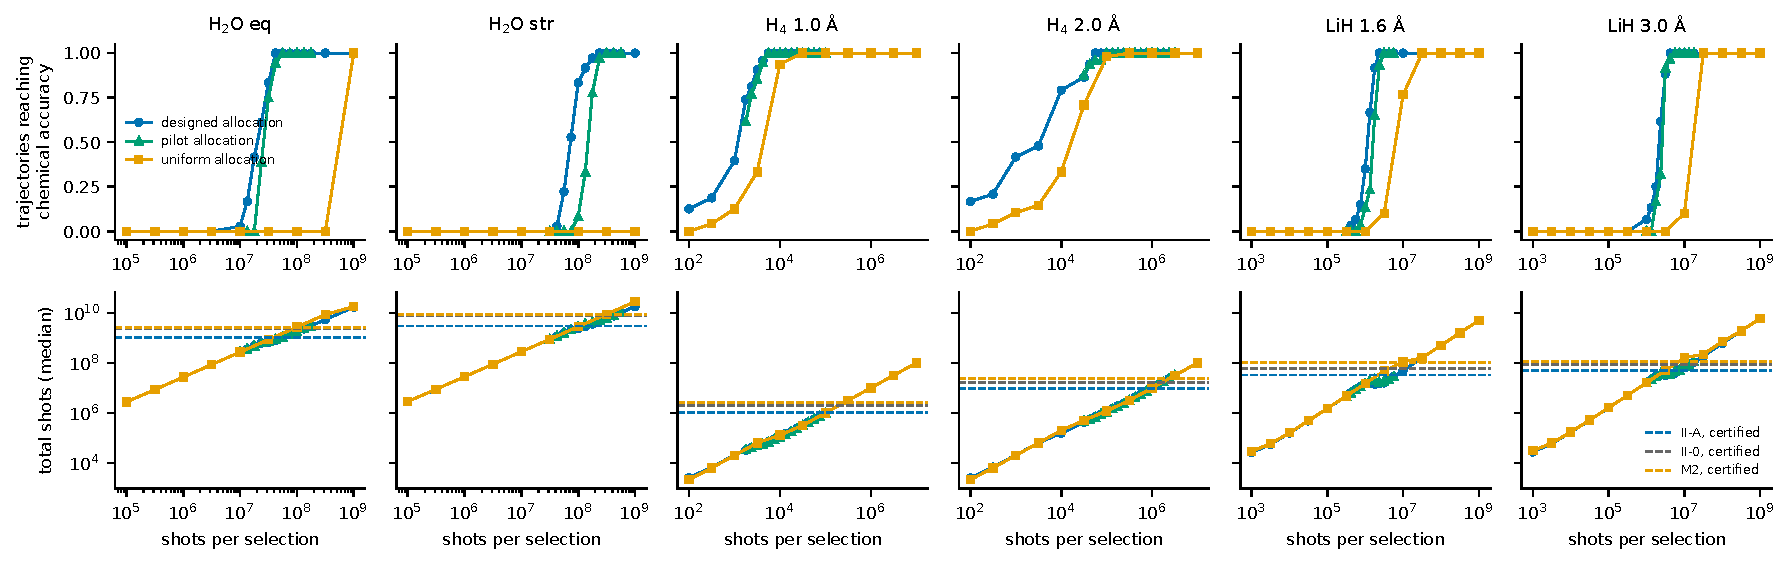
\includegraphics[width=\textwidth]{figures/fig_fixed_budget}
\caption{Fixed-budget selection along ADAPT trajectories. Top: share of trajectories reaching chemical accuracy against shots per selection. Bottom: median total shots; dashed lines are the certified methods (II-A, II-0 and M2).}
\label{fig:fixedbudget}
\end{figure*}

On the small systems the certification is expensive (Table~\ref{tab:fixedbudget}, Fig.~\ref{fig:fixedbudget}). On H$_4$ at 1.0~\AA\ a fixed budget of $1.3\times10^{4}$ shots per selection reaches chemical accuracy in $10.9$ steps (exact: 10) in all 96 trajectories at a total of $1.5\times10^{5}$ shots, $7.2$ times below the certified II-A ($1.1\times10^{6}$), $13$ times below II-0 and $18$ times below M2; at 2.0~\AA\ the premium of II-A is $6.4$, and on LiH at 1.6~\AA\ $2.1$. On LiH at 3.0~\AA\ the two cost the same ($1.0$), and on both H$_2$O geometries the certified II-A is the cheaper by a factor of $2$ to $3$ ($0.5$ and $0.4$ of the fixed total); the certified II-0 and M2 cost $1.0$--$1.2$ times the fixed budget there and $1.6$ and $2.2$ times on LiH at 3.0~\AA. The pilot allocation, which needs no exact variance, adequate at the same budget or one step of the grid higher, costs $0.9$--$1.4$ times the designed allocation, so the comparison does not rest on exact variances. The uniform allocation needs $10$--$13$ times more shots per selection on LiH and, on H$_2$O, did not reach chemical accuracy within one step of exact ADAPT up to $10^{9}$ shots per selection. The premium depends strongly on the tolerance $\rho$ of the certified selection (Table~\ref{tab:fixedrho}): on H$_4$ it falls from $25$ at $\rho=0.05$ to $1.8$ and $1.1$ at $\rho=0.3$ (the two geometries), on LiH at 1.6~\AA\ from $3.7$ to $1.0$, and on LiH at 3.0~\AA\ and H$_2$O the certified II-A is below the fixed budget at every $\rho$ from $0.1$ (at $\rho=0.05$ on LiH $1.3$). The certified trajectories at the other tolerances took on average within $0.1$ steps of exact ADAPT's number, so a looser tolerance did not cost steps in these systems.

\begin{table}[!htb]
\centering\small
\caption{Certified II-A and II-0 along the ADAPT trajectories at four tolerances $\rho$ (median total selection shots, mean steps in brackets) against the cheapest adequate fixed budget (designed allocation), which does not depend on $\rho$. Stretched H$_2$O at $\rho=0.2$ and $0.3$ was still running when the table was made.}
\label{tab:fixedrho}
\footnotesize\setlength{\tabcolsep}{3pt}
\fitcol{%
% BEGIN INLINE tab_fixed_rho
\begin{tabular}{@{}lrrrrr@{}}
\toprule
System & $\rho$ & II-A total (steps) & II-0 total (steps) & fixed total & II-A / fixed \\
\midrule
H$_2$O eq & 0.1 & $1.1\times10^{9}$ (17.0) & $2.5\times10^{9}$ (17.0) & $2.3\times10^{9}$ & 0.47 \\
 & 0.2 & $7.0\times10^{8}$ (17.0) & $2.1\times10^{9}$ (17.0) & $2.3\times10^{9}$ & 0.31 \\
 & 0.3 & $5.8\times10^{8}$ (17.0) & $1.9\times10^{9}$ (17.0) & $2.3\times10^{9}$ & 0.26 \\
\midrule
H$_2$O str & 0.1 & $3.0\times10^{9}$ (18.0) & $7.9\times10^{9}$ (18.0) & $7.6\times10^{9}$ & 0.39 \\
 & 0.2 & -- & $7.5\times10^{9}$ (18.0) & $7.6\times10^{9}$ & -- \\
 & 0.3 & -- & $6.6\times10^{9}$ (18.0) & $7.6\times10^{9}$ & -- \\
\midrule
H$_4$ 1.0 \AA & 0.05 & $3.7\times10^{6}$ (10.0) & $5.8\times10^{6}$ (10.0) & $1.5\times10^{5}$ & 25.19 \\
 & 0.1 & $1.1\times10^{6}$ (10.0) & $1.9\times10^{6}$ (10.0) & $1.5\times10^{5}$ & 7.16 \\
 & 0.2 & $3.9\times10^{5}$ (10.0) & $6.3\times10^{5}$ (10.0) & $1.5\times10^{5}$ & 2.64 \\
 & 0.3 & $2.7\times10^{5}$ (10.0) & $4.3\times10^{5}$ (10.0) & $1.5\times10^{5}$ & 1.83 \\
\midrule
H$_4$ 2.0 \AA & 0.05 & $3.7\times10^{7}$ (10.0) & $4.9\times10^{7}$ (10.0) & $1.5\times10^{6}$ & 25.41 \\
 & 0.1 & $9.4\times10^{6}$ (10.0) & $1.6\times10^{7}$ (10.0) & $1.5\times10^{6}$ & 6.39 \\
 & 0.2 & $2.9\times10^{6}$ (10.0) & $5.1\times10^{6}$ (10.0) & $1.5\times10^{6}$ & 1.99 \\
 & 0.3 & $1.6\times10^{6}$ (10.0) & $2.9\times10^{6}$ (10.0) & $1.5\times10^{6}$ & 1.07 \\
\midrule
LiH 1.6 \AA & 0.05 & $5.8\times10^{7}$ (5.0) & $1.1\times10^{8}$ (5.0) & $1.6\times10^{7}$ & 3.69 \\
 & 0.1 & $3.3\times10^{7}$ (5.0) & $6.0\times10^{7}$ (5.0) & $1.6\times10^{7}$ & 2.08 \\
 & 0.2 & $2.0\times10^{7}$ (5.0) & $4.4\times10^{7}$ (5.0) & $1.6\times10^{7}$ & 1.26 \\
 & 0.3 & $1.6\times10^{7}$ (5.0) & $3.8\times10^{7}$ (5.0) & $1.6\times10^{7}$ & 1.03 \\
\midrule
LiH 3.0 \AA & 0.05 & $6.8\times10^{7}$ (6.0) & $1.2\times10^{8}$ (6.0) & $5.2\times10^{7}$ & 1.29 \\
 & 0.1 & $5.0\times10^{7}$ (6.1) & $8.3\times10^{7}$ (6.0) & $5.2\times10^{7}$ & 0.95 \\
 & 0.2 & $2.3\times10^{7}$ (6.1) & $4.9\times10^{7}$ (6.0) & $5.2\times10^{7}$ & 0.43 \\
 & 0.3 & $1.5\times10^{7}$ (6.1) & $4.2\times10^{7}$ (6.2) & $5.2\times10^{7}$ & 0.29 \\
\bottomrule
\end{tabular}
% END INLINE tab_fixed_rho

}
\end{table}

Two things limit what this comparison shows. A fixed budget certifies nothing: at the adequate budgets only $76$--$95\%$ of its selections were within $\rho=0.1$ of the best generator ($83$--$84\%$ on H$_4$ at 1.0~\AA, $90$--$92\%$ at 2.0~\AA, $76$--$84\%$ on LiH at 1.6~\AA, $87$--$89\%$ at 3.0~\AA, $88$--$95\%$ on H$_2$O), against at least $98.7\%$ for the certified II-0 and II-A, and the budget that works is found by running the trajectory with the answer known. The premium measures the cost of the guarantee, not a procedure that could be followed. With these qualifications, the value of the method on small, wide-gap problems is the guarantee and not a saving, and on the larger systems it is also a saving.

\subsection{Q11: How sensitive are the results to the settings, and what is the scale of the computation?}
\label{sec:q11}

\paragraph{Thresholds.} The thresholds of the method (50 shots before a context carries learned coefficients and before a held-out covariance is used, the refit factor of 1.5) were fixed before the experiments. Table~\ref{tab:thresholds} varies them on three states. Lowering the minimum number of shots to 20 changes the cost of II-A by $0.78$--$0.93$, raising it to 100 or 200 raises the cost by $1.16$--$1.35$ and $1.62$--$1.99$ on these early states; refit factors of 1.25, 2 and 3 change it by $0.95$--$0.98$, $1.06$--$1.10$ and $1.15$--$1.20$. On the late states the minimum matters in the opposite direction (Q9): there a minimum of 200 or 400 shots \emph{lowers} the cost by a factor of $4$--$7$ because the learned variance is no longer underestimated. The dependence is therefore state-dependent and the default of 50 shots is not optimal for the late states of an ADAPT run; a rule that raises the minimum with the number of candidates still alive, or a small-sample bound on the variance, is the natural remedy. Every selection was correct in all trials of the three early states at every setting.

\begin{table}[!htb]
\centering\small
\caption{II-A (a priori start, sign-aware rule, 200 trials) with other thresholds: mean context-shots at the default (50 shots, refit factor 1.5), and the ratio to it for minimum shots of 20, 100 and 200, and refit factors of 1.25, 2 and 3; smallest share of correct selections over all settings in the last column.}
\label{tab:thresholds}
\fitcol{%
% BEGIN INLINE tab_sensitivity_thresholds
\begin{tabular}{@{}lrrrrrrrr@{}}
\toprule
State & default 50 / 1.5 & min shots 20 & 100 & 200 & refit 1.25 & 2 & 3 & correct, all (\%) \\
\midrule
H$_4$ 1.0~\AA, CISD & $2.61\times10^{4}$ & 0.93 & 1.16 & 1.62 & 0.98 & 1.10 & 1.15 & 100 \\
H$_4$ 2.0~\AA, CISD & $1.35\times10^{4}$ & 0.93 & 1.35 & 1.99 & 0.95 & 1.06 & 1.20 & 100 \\
LiH 3.0~\AA, HF & $3.09\times10^{5}$ & 0.78 & 1.33 & 1.89 & 0.98 & 1.09 & 1.15 & 100 \\
\bottomrule
\end{tabular}
% END INLINE tab_sensitivity_thresholds

}
\end{table}

\paragraph{Tolerance $\rho$.} On fixed states the cost falls as $\rho$ grows on H$_4$ (II-A: $2.6\times10^{4}$ at $\rho=0$ to $2.0\times10^{4}$ at $0.3$) and not at all on LiH at 3.0~\AA, where the gap is large. Along trajectories it falls faster (Table~\ref{tab:fixedrho}): for II-A on H$_4$ at 1.0~\AA\ the total is $3.7\times10^{6}$, $1.1\times10^{6}$, $3.9\times10^{5}$ and $2.7\times10^{5}$ shots at $\rho=0.05$, $0.1$, $0.2$ and $0.3$, and the ratio II-A/II-0 stays between $0.37$ and $0.77$ on H$_4$ and LiH at every tolerance; on H$_2$O at equilibrium it is $0.43$, $0.34$ and $0.30$ at $0.1$, $0.2$ and $0.3$.

\paragraph{Scale.} The structure of the problem and the cost of the classical design grow with the molecule (Table~\ref{tab:scaling}). From H$_4$ to N$_2$ in STO-3G (8 to 20 qubits) the pool grows from 26 to 609 generators, the Pauli products of the commutators from $1.3\times10^{3}$ to $7.4\times10^{5}$, the measurement contexts from 53 to $1.5\times10^{4}$ and the two-qubit gates per circuit from 8 to 72; the coordinates of one II-A design problem grow from 308 to $1.9\times10^{4}$ per generator. We added a case in a larger basis: H$_2$O in cc-pVDZ restricted to a window of eight orbitals (the frozen-core Hamiltonian of the four occupied orbitals and four virtual ones, two of $a_1$ and two of in-plane $b$ symmetry, after the larger-basis note of our colleagues; 16 qubits, $K=360$, $2.2\times10^{5}$ products, 5{,}408 contexts, 44 two-qubit gates per circuit). One refit of all generators takes seconds on H$_4$ and LiH (13--17 s for $K=92$), about 30 s on BeH$_2$ and H$_2$O, a little over a minute for the cc-pVDZ window and $5.5$ minutes for N$_2$ ($0.54$ s per generator for 609 generators). One complete II-A selection costs $3$ s (H$_4$), $137$--$191$ s (LiH), about 17 min (BeH$_2$) and 74 min (H$_2$O, STO-3G) of classical time on one core. Building the problem (the commutator expansions) took $8.4$ h serially for N$_2$; we distributed the generators over processes, which gave the cc-pVDZ window in two minutes on a cluster node, with identical results. The simulation of the 20-qubit state needs 250 GB, which is why the shot-level comparison of this work stops at 14 qubits; the exact ADAPT trajectory of the cc-pVDZ window is still $5.9$~mHa (equilibrium) and $3.7$~mHa (stretched) from FCI after the 40 steps we allowed, with gradients above $3\times10^{-2}$, which is why no measured trajectory is reported for it. These timings are for the classical design on one core; nothing here is a measurement of the quantum cost, and larger molecules are not tested at shot level.

\begin{table*}[!htb]
\centering\small
\caption{Structure and classical cost of the design (HF state, UCCSD pool, strategy of the main study; all but the last two rows in STO-3G). II-A, one selection: mean classical seconds of one selection on a fixed state of the molecule (design, statistics, allocation); `--' where no fixed-state selection was run.}
\label{tab:scaling}
\footnotesize\setlength{\tabcolsep}{4pt}
% BEGIN INLINE tab_scaling
\begin{tabular}{@{}lrrrrrrr@{}}
\toprule
System & qubits & $K$ & Pauli products & contexts & CZ per circuit & coordinates per generator & II-A, one selection (s) \\
\midrule
H$_4$ & 8 & 26 & 1{,}276 & 53 & 8.4 & 308 & 3 \\
LiH 3.0 & 12 & 92 & 30{,}196 & 980 & 23.3 & 4{,}082 & 191 \\
LiH 1.6 & 12 & 92 & 30{,}196 & 980 & 23.3 & 4{,}078 & 137 \\
H$_6$ chain & 12 & 117 & 35{,}094 & 1{,}054 & 23.0 & 6{,}441 & -- \\
BeH$_2$ & 14 & 204 & 85{,}487 & 2{,}450 & 33.3 & 4{,}371 & 1028 \\
H$_2$O STO-3G & 14 & 140 & 81{,}566 & 2{,}366 & 32.2 & 7{,}483 & 4442 \\
H$_2$O cc-pVDZ (8 orbitals) & 16 & 360 & 220{,}355 & 5{,}408 & 44.2 & 13{,}643 & -- \\
N$_2$ STO-3G & 20 & 609 & 740{,}431 & 14{,}931 & 72.2 & 19{,}458 & -- \\
\bottomrule
\end{tabular}
% END INLINE tab_scaling

\end{table*}

\subsection{Q12: Do the baselines and the optimization cost hold up against independent checks?}
\label{sec:q12}

\paragraph{Reproducing the published baseline.} The successive-elimination baseline was implemented from the description of Huang and Izmaylov~\cite{huang2026} (qubit-wise commuting fragments by sorted insertion, exact fragment variances in a Gaussian model, $\varepsilon'_r=(5-2r/5)\varepsilon$, $R_r=8\varepsilon'_r$, at most ten rounds, linear molecules with 1~\AA\ between adjacent atoms, UCCSD pool, chemical accuracy $1.59$~mHa) and compared with the reduction in measurements they report against estimating every fragment to a fixed precision. Their paper does not say whether the samples of earlier rounds are kept, so we ran both variants (Table~\ref{tab:reproduction}, 10 seeds). With fresh samples in every round the reductions are $91.8\pm2.0\%$ for H$_4$ (published $93.0\%$), $80.7\pm7.8\%$ for LiH ($80.8\%$) and $90.3\pm4.9\%$ for BeH$_2$ ($90.0\%$), within one standard deviation of the published values; with the samples kept they are higher ($93.0$, $89.5$ and $93.1\%$). We read the first variant as the reading of their method that our implementation reproduces, and the second as a stronger baseline than the published one. Only the UCCSD pool and the particle-number sector were reproduced; the qubit and qubit-excitation pools were not.

\begin{table}[!htb]
\centering\small
\caption{Percentage reduction of the measurements needed for selection to chemical accuracy relative to estimating every fragment to a fixed precision: Huang and Izmaylov's Table~I (UCCSD pool) and our implementation of their method (mean $\pm$ s.d. over 10 seeds), with the samples of earlier rounds kept or with fresh samples in every round.}
\label{tab:reproduction}
\fitcol{%
% BEGIN INLINE tab_reproduction
\begin{tabular}{@{}lrrr@{}}
\toprule
System & published (\%) & reproduced, samples kept (\%) & reproduced, fresh each round (\%) \\
\midrule
H$_4$ & 93.0 & 93.0 $\pm$ 1.0 & 91.8 $\pm$ 2.0 \\
LiH & 80.8 & 89.5 $\pm$ 6.5 & 80.7 $\pm$ 7.8 \\
BeH$_2$ & 90.0 & 93.1 $\pm$ 0.7 & 90.3 $\pm$ 4.9 \\
\bottomrule
\end{tabular}
% END INLINE tab_reproduction

}
\end{table}

\paragraph{A sampled optimizer.} Q7 used a model of the optimization cost, which Sec.~\ref{sec:resources} calls likely to be an underestimate. We replaced it by a measurement: coordinate-wise updates of the parameters along the exact ADAPT trajectory (the energy is a trigonometric polynomial of degree two in each parameter, so five noisy energy estimates per parameter fix its minimum), with the energy estimated to $\varepsilon_E$, the shots counted as energy evaluations times $(1~\mathrm{mHa}/\varepsilon_E)^{2}$ times the shots of an energy of 1~mHa. Table~\ref{tab:sampledopt} compares the shots with the model $C_{\mathrm{opt}}$ of Sec.~\ref{sec:resources} for $\eta=2$ and $\eta=4$. For $\varepsilon_E=1$~mHa the sampled cost is $0.23$ ($0.12$ for $\eta=4$) of the model on H$_4$ and $0.46$ ($0.24$) on LiH, but the optimization then reaches chemical accuracy in all runs only on H$_4$ ($100\%$) and in $50\%$ of the runs on LiH. When the optimizer must reach chemical accuracy reliably, $\varepsilon_E$ has to go down to $0.1$~mHa on LiH ($100\%$ of the runs), and the cost is $31$--$71$ times the model's with $\eta=2$ ($16$--$38$ with $\eta=4$), at $5\times10^{10}$ shots. The model therefore underestimates the optimization cost when chemical accuracy is required under sampling noise, and the conclusion of Q7, that optimization and not selection sets the cost of a complete run, is stronger with the sampled optimizer, not weaker. The final energies of the sampled runs lie within $0.2$~mHa of those of the exact optimizer.

\begin{table}[!htb]
\centering\small
\caption{Sampled optimization along the exact ADAPT trajectory (10 seeds): energy evaluations, total shots, the ratio to the model $C_{\mathrm{opt}}$ ($\eta=2$ / $\eta=4$) and the mean final error.}
\label{tab:sampledopt}
\fitcol{%
% BEGIN INLINE tab_sampled_optimizer
\begin{tabular}{@{}lrrrrr@{}}
\toprule
System & $\varepsilon_E$ (mHa) & energies & sampled shots & model $\eta=2$ / $\eta=4$ & final $\Delta E$ (mHa) \\
\midrule
H$_4$ 1.0~\AA & 1 & 672 & $3.71\times10^{8}$ & 0.23 / 0.12 & 1.23 \\
H$_4$ 1.0~\AA & 0.3 & 744 & $4.55\times10^{9}$ & 2.86 / 1.49 & 1.16 \\
H$_4$ 1.0~\AA & 0.1 & 897 & $4.97\times10^{10}$ & 31.28 / 16.25 & 1.09 \\
LiH 3.0~\AA & 1 & 255 & $3.06\times10^{8}$ & 0.46 / 0.24 & 1.53 \\
LiH 3.0~\AA & 0.3 & 314 & $4.22\times10^{9}$ & 6.27 / 3.31 & 1.29 \\
LiH 3.0~\AA & 0.1 & 391 & $4.80\times10^{10}$ & 71.45 / 37.67 & 0.85 \\
\bottomrule
\end{tabular}
% END INLINE tab_sampled_optimizer

}
\end{table}
% END REFEREE RESULTS
\section{Discussion}
\label{sec:discussion}

\paragraph{What was compared, and how faithfully.} The baselines are our implementations, and three of them differ from the originals in ways that matter. (i)~The pivot grouping of Anastasiou \textit{et al.}~\cite{anastasiou2023}, which the published version of the shot-reuse work finds to be the dominant reduction~\cite{ikhtiarudin2025}, is cheap in circuit depth and dear in shots: as published it needs $12.8$ times the shots of the same estimator on first-fit contexts on H$_4$ (sequential $7.1\times10^{5}$ against $5.6\times10^{4}$; static $12.8$ times) and $21$ times on LiH (sequential $1.8\times10^{7}$ against $8.3\times10^{5}$; static $5.7$ times), as their own estimate of $4n_q$ energy evaluations for the whole pool implies. Reading each product from one pivot context (``merged'') removes most of the loss ($1.7$ and $5.3$ times sequential, $1.6$ and $1.2$ times static, on H$_4$ and LiH) but is not their scheme. (ii)~Huang and Izmaylov's QWC fragments~\cite{huang2026} cost almost the same as our fully commuting ones when each gradient is measured on its own: $1.02$ to $1.18$ times on LiH and H$_2$O and $1.9$ to $2.0$ times on H$_4$ (over the nine fixed states of Q8), so the independent baseline we used is not a strawman for the original, and it has no entangling gate. (iii)~The QWC cliques of the reuse baseline are measured in a product basis, with no entangling gate, as in the original. A fourth difference favors the baselines: all of them are given the optimal allocation of Eq.~\eqref{eq:alloc} and the same radii as our methods, whereas the originals use heuristic schedules or variance bounds.

% BEGIN GENERATED disc_depth
\begin{table*}[!htb]
\centering\small
\caption{Shots against measurement-circuit depth. Every method on every family of measurement contexts: mean context-shots over trials, mean two-qubit gates per shot, and the gain of II-A over the sequential M1 on the same contexts. Blocks of $b$ qubits commute block by block, so each circuit is a product of Cliffords on $b$ qubits (at most $b(b-1)/2$ CZ per block); blocks of one qubit are qubit-wise commuting, and the pivot contexts are those of Anastasiou \textit{et al.} The rows of independent arms give the cost of independent BAI (M2) in the column of the sequential M1, and a dash marks the columns that do not apply to it; $^\ddagger$its ratio is to II-A on the same family of contexts (fully commuting or qubit-wise commuting). $^\dagger$Sign-aware rule, and the sign-aware M1 seq in the ratio: on the published pivot contexts every product is measured in several contexts with few shots each, the plug-in variances of such contexts are unreliable, and the pairwise II-A selected the wrong generator in 34\% of the trials on H$_4$ 1.0 CISD and 76\% of the trials on LiH HF.}
\label{tab:depth}
\begin{tabular}{lrrrrrr}
\toprule
contexts & CZ / shot & M1 static & M1 seq & II-0 & II-A & M1 seq / II-A \\
\midrule
\multicolumn{7}{l}{\emph{H$_4$ 1.0 CISD}} \\
qubit-wise (blocks of 1) & 0.0 & $1.20\times10^{5}$ & $1.13\times10^{5}$ & 80\,015 & 61\,410 & 1.84 \\
blocks of 2 qubits & 1.4 & 98\,879 & 86\,384 & 62\,659 & 50\,478 & 1.71 \\
blocks of 4 qubits & 4.5 & 71\,065 & 63\,698 & 48\,622 & 39\,899 & 1.60 \\
fully commuting & 8.2 & 59\,671 & 55\,870 & 41\,463 & 27\,129 & 2.06 \\
pivot, as published & 6.2 & $7.63\times10^{5}$ & $7.15\times10^{5}$ & $5.09\times10^{5}$ & $1.10\times10^{5}$$^\dagger$ & 6.71$^\dagger$ \\
pivot, merged & 6.1 & 98\,132 & 96\,840 & 68\,423 & 44\,917 & 2.16 \\
M2 FC (independent arms) & 5.7 & -- & $1.01\times10^{5}$ & -- & -- & 3.73$^\ddagger$ \\
M2 QWC (independent arms) & 0.0 & -- & $1.96\times10^{5}$ & -- & -- & 3.19$^\ddagger$ \\
\midrule
\multicolumn{7}{l}{\emph{LiH HF}} \\
qubit-wise (blocks of 1) & 0.0 & $5.29\times10^{6}$ & $5.93\times10^{6}$ & $5.29\times10^{5}$ & $3.63\times10^{5}$ & 16.33 \\
blocks of 2 qubits & 2.6 & $5.03\times10^{6}$ & $1.40\times10^{6}$ & $5.33\times10^{5}$ & $3.64\times10^{5}$ & 3.85 \\
blocks of 4 qubits & 6.2 & $4.20\times10^{6}$ & $1.13\times10^{6}$ & $3.99\times10^{5}$ & $3.10\times10^{5}$ & 3.64 \\
fully commuting & 21.0 & $3.56\times10^{6}$ & $8.33\times10^{5}$ & $3.05\times10^{5}$ & $1.85\times10^{5}$ & 4.52 \\
pivot, as published & 7.5 & $2.01\times10^{7}$ & $1.78\times10^{7}$ & $3.28\times10^{6}$ & $9.08\times10^{5}$$^\dagger$ & 16.79$^\dagger$ \\
pivot, merged & 9.7 & $4.18\times10^{6}$ & $4.44\times10^{6}$ & $6.69\times10^{5}$ & $3.95\times10^{5}$ & 11.23 \\
M2 FC (independent arms) & 7.9 & -- & $1.01\times10^{6}$ & -- & -- & 5.45$^\ddagger$ \\
M2 QWC (independent arms) & 0.0 & -- & $1.14\times10^{6}$ & -- & -- & 3.13$^\ddagger$ \\
\midrule
\multicolumn{7}{l}{\emph{H$_2$O eq CISD}} \\
qubit-wise (blocks of 1) & 0.0 & $4.35\times10^{11}$ & $1.34\times10^{11}$ & $2.11\times10^{10}$ & $1.21\times10^{10}$ & 11.10 \\
fully commuting & 30.3 & $4.12\times10^{11}$ & $9.42\times10^{10}$ & $2.05\times10^{10}$ & $8.80\times10^{9}$ & 10.70 \\
M2 FC (independent arms) & 8.5 & -- & $3.70\times10^{10}$ & -- & -- & 4.21$^\ddagger$ \\
M2 QWC (independent arms) & 0.0 & -- & $3.84\times10^{10}$ & -- & -- & 3.19$^\ddagger$ \\
\midrule
\multicolumn{7}{l}{\emph{H$_2$O str CISD}} \\
qubit-wise (blocks of 1) & 0.0 & $6.34\times10^{9}$ & $9.76\times10^{8}$ & $8.80\times10^{7}$ & $6.06\times10^{7}$ & 16.11 \\
fully commuting & 29.4 & $5.72\times10^{9}$ & $1.49\times10^{9}$ & $8.63\times10^{7}$ & $3.95\times10^{7}$ & 37.70 \\
M2 FC (independent arms) & 10.1 & -- & $1.30\times10^{8}$ & -- & -- & 3.28$^\ddagger$ \\
M2 QWC (independent arms) & 0.0 & -- & $1.32\times10^{8}$ & -- & -- & 2.17$^\ddagger$ \\
\bottomrule
\end{tabular}
\end{table*}
% END GENERATED disc_depth

\begin{figure*}[!htb]
\centering
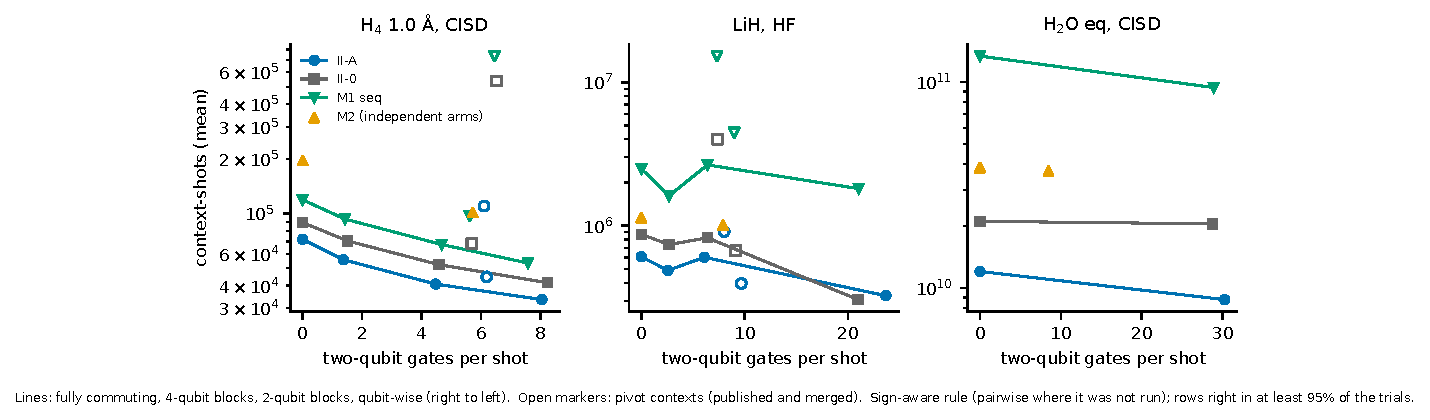
\includegraphics[width=\textwidth]{figures/fig_depth}
\caption{Context-shots against two-qubit gates per shot for II-A, II-0, M1 seq and M2 on four families of contexts (lines, from fully commuting at the right to qubit-wise at the left) and the pivot contexts (open markers). Sign-aware rule where the pairwise rule was not run; only rows correct in at least 95\% of the trials.}
\label{fig:depth}
\end{figure*}

\paragraph{Shots against circuit depth.} The learned designs are not tied to the deep circuits of the fully commuting contexts (Table~\ref{tab:depth}). With product measurements and no entangling gate II-A needs $6.1\times10^{4}$ shots on H$_4$ and $3.6\times10^{5}$ on LiH, against $2.0\times10^{5}$ and $1.1\times10^{6}$ for independent BAI with QWC fragments, the form of Huang and Izmaylov: $3.2$ and $3.1$ times fewer ($1.9$ times on LiH with the sign-aware rule). Over the seven fixed states of this comparison (H$_4$ at both geometries, LiH at the Hartree--Fock state and after three and five ADAPT steps, H$_2$O at both geometries; the table shows four of them) the factor is $1.1$ to $4.1$. The relevant comparison for the cost of giving up depth is with the best baseline that is allowed the full depth. II-A on product measurements needs $1.1$ and $1.2$ times more shots than that baseline on H$_4$ at the two geometries ($5.6\times10^{4}$ for the sequential M1 at 1.0~\AA), $2.3$ and $1.5$ times fewer on LiH at the Hartree--Fock state ($8.3\times10^{5}$) and after three steps, $3.1$ and $2.1$ times fewer on H$_2$O, and $1.02$ times more on LiH after five steps. On product measurements the learned designs therefore stay within $22\%$ of the best deep-circuit baseline on H$_4$ and on LiH after five steps and beat it on the other four states.

LiH after five steps is also the exception to the gain of the learned splitting on product measurements. II-A costs $2.2$ times more there than on fully commuting contexts, and its mean ($9.6\times10^{7}$) does not differ from that of II-0 ($9.3\times10^{7}$) within the standard errors ($7\times10^{6}$ and $4\times10^{6}$), although its median is $17\%$ lower ($6.9\times10^{7}$ against $8.3\times10^{7}$). Five of the $100$ trials, with seven or eight refits against a median of five, cost $2.6$ to $3.9\times10^{8}$ shots, and without them the means are $8.4\times10^{7}$ and $8.7\times10^{7}$. On fully commuting contexts II-A is $34\%$ below II-0 on the same state. We have not found why product measurements remove the gain here.

\paragraph{Intermediate depths and the published pivot contexts.} From $0$ to $8$ ($21$ on LiH) two-qubit gates per circuit the cost of II-A falls by $2.3$ ($2.0$ on LiH). Blocks of four qubits ($4.5$ and $6.2$ gates) give about half of that gain on H$_4$ and a quarter on LiH, and on both molecules the merged pivot contexts need more shots and more gates than blocks of four qubits ($4.5\times10^{4}$ at $6.1$ gates against $4.0\times10^{4}$ at $4.5$ on H$_4$, $4.0\times10^{5}$ at $9.7$ against $3.1\times10^{5}$ at $6.2$ on LiH). On the pivot contexts as published, where every pivot that produces a product measures it, II-0 needs $5.1\times10^{5}$ shots on H$_4$ and $3.3\times10^{6}$ on LiH, $1.4$ and $5.4$ times fewer than the sequential M1, and II-A with the sign-aware rule needs $1.1\times10^{5}$ and $9.1\times10^{5}$, $6.7$ and $17$ times fewer than the sequential M1 with that rule. The pairwise II-A is not valid on these contexts: it selected a wrong generator in $34\%$ of the trials on H$_4$ and $76\%$ on LiH, because each product is measured in several contexts with few shots each and the plug-in variances of such contexts are unreliable, which the sign-aware rule bounds. On H$_2$O, shared elimination with fixed estimators (II-0) needs the same number of shots on QWC contexts as on fully commuting ones ($2.1\times10^{10}$ against $2.05\times10^{10}$ at equilibrium, $8.8\times10^{7}$ against $8.6\times10^{7}$ stretched), and $1.8$ and $1.5$ times fewer than independent BAI with QWC fragments ($3.8\times10^{10}$ and $1.3\times10^{8}$). The learned splitting on product measurements needs $1.2\times10^{10}$ and $6.1\times10^{7}$ shots there, $3.2$ and $2.2$ times fewer than independent BAI with QWC fragments and $1.4$ and $1.5$ times the cost on fully commuting contexts ($8.8\times10^{9}$ and $3.95\times10^{7}$).

\paragraph{Gate errors.} How much of the depth is worth having depends on the gate error (Table~\ref{tab:noise}). With a depolarizing error $p_2$ after every CZ, no selection went wrong because of it up to $p_2=0.06$ on H$_4$ and LiH, but the cost of the deep contexts grows. On H$_4$, II-A on fully commuting contexts costs $1.5$ times more at $p_2=0.03$ and $3.2$ times more at $0.06$ than at $0.003$, while product measurements do not change. At $p_2=0.03$ the fully commuting contexts are still ahead ($4.2\times10^{4}$ against $6.0\times10^{4}$ shots), and they are overtaken at about $p_2=0.04$. Bansingh \textit{et al.}~\cite{bansingh2022} include the same effect for the energy and find the non-local groupings still ahead after the gate errors are counted. On LiH, with $21$ gates per circuit, II-A changes by $3\%$ up to $p_2=0.03$ and by $13\%$ at $0.06$ ($2.3\times10^{5}$ against $3.7\times10^{5}$ on product measurements), so there the fully commuting contexts stay ahead.

\paragraph{Limits of the noise model.} The same gate errors would also corrupt the preparation circuit, which the present model leaves noiseless, and Dalton \textit{et al.} find that the best-performing variational algorithms need gate-error probabilities between $10^{-6}$ and $10^{-4}$ without error mitigation to reach chemical accuracy for small molecules~\cite{dalton2024}. The sweep of $p_2$ is therefore a sensitivity study of the measurement circuits, not a prediction for a device. The model multiplies each Pauli expectation value by a factor between zero and one that depends on the product and on its circuit. It keeps every sign but does not guarantee the ranking of the candidates, although no selection went wrong in our tests, and the selection criterion is known to be resilient to some noise channels~\cite{haravu2026}. Coherent errors, which can prevent the selection from converging~\cite{haravu2026}, are not modeled and would call for radii that include a bias.

% BEGIN GENERATED disc_noise
\begin{table*}[!htb]
\centering\small
\caption{Noisy measurement circuits. A depolarizing error of probability $p_2$ after every CZ gate; each cell is the share of selections that picked the exact best generator (of the noiseless gradients) and the mean cost. The intervals know shot noise only.}
\label{tab:noise}
\begin{tabular}{lrrrrr}
\toprule
contexts and method & CZ & $p_2=0.003$ & $p_2=0.01$ & $p_2=0.03$ & $p_2=0.06$ \\
\midrule
\multicolumn{6}{l}{\emph{H$_4$ 1.0 CISD}} \\
M1 seq, FC & 7.9 & 100\% / 56\,544 & 100\% / 58\,607 & 100\% / 88\,949 & 100\% / $1.46\times10^{5}$ \\
II-A, FC & 7.9 & 100\% / 27\,954 & 100\% / 31\,253 & 100\% / 41\,722 & 100\% / 90\,710 \\
II-A, blocks of 4 & 4.5 & 100\% / 41\,076 & 100\% / 42\,677 & 100\% / 45\,477 & 100\% / 59\,721 \\
II-A, blocks of 2 & 1.4 & 100\% / 48\,159 & 100\% / 49\,770 & 100\% / 53\,544 & 100\% / 56\,655 \\
II-A, QWC & 0.0 & 100\% / 59\,785 & 100\% / 59\,785 & 100\% / 59\,785 & 100\% / 59\,785 \\
M1 seq, QWC & 0.0 & 100\% / $1.10\times10^{5}$ & 100\% / $1.10\times10^{5}$ & 100\% / $1.10\times10^{5}$ & 100\% / $1.10\times10^{5}$ \\
II-A, pivot contexts & 6.1 & 100\% / 43\,409 & 100\% / 47\,788 & 100\% / 55\,026 & 100\% / 82\,711 \\
M2, FC & 5.6 & 100\% / $1.47\times10^{5}$ & 100\% / $1.51\times10^{5}$ & 100\% / $1.59\times10^{5}$ & 100\% / $1.85\times10^{5}$ \\
M2, QWC & 0.0 & 100\% / $3.45\times10^{5}$ & 100\% / $3.45\times10^{5}$ & 100\% / $3.45\times10^{5}$ & 100\% / $3.45\times10^{5}$ \\
\multicolumn{6}{l}{\emph{LiH HF}} \\
M1 seq, FC & 21.1 & 100\% / $8.02\times10^{5}$ & 100\% / $8.53\times10^{5}$ & 100\% / $8.54\times10^{5}$ & 100\% / $1.04\times10^{6}$ \\
II-A, FC & 21.1 & 100\% / $1.99\times10^{5}$ & 100\% / $2.00\times10^{5}$ & 100\% / $2.05\times10^{5}$ & 100\% / $2.25\times10^{5}$ \\
II-A, blocks of 4 & 6.2 & 100\% / $2.96\times10^{5}$ & 100\% / $2.98\times10^{5}$ & 100\% / $3.15\times10^{5}$ & 100\% / $3.17\times10^{5}$ \\
II-A, blocks of 2 & 2.6 & 100\% / $3.60\times10^{5}$ & 100\% / $3.68\times10^{5}$ & 100\% / $3.47\times10^{5}$ & 100\% / $3.58\times10^{5}$ \\
II-A, QWC & 0.0 & 98\% / $3.71\times10^{5}$ & 98\% / $3.71\times10^{5}$ & 98\% / $3.71\times10^{5}$ & 98\% / $3.71\times10^{5}$ \\
M1 seq, QWC & 0.0 & 98\% / $5.74\times10^{6}$ & 98\% / $5.74\times10^{6}$ & 98\% / $5.74\times10^{6}$ & 98\% / $5.74\times10^{6}$ \\
M2, FC & 8.0 & 100\% / $1.68\times10^{6}$ & 100\% / $1.72\times10^{6}$ & 100\% / $1.82\times10^{6}$ & 100\% / $1.98\times10^{6}$ \\
M2, QWC & 0.0 & 100\% / $1.90\times10^{6}$ & 100\% / $1.90\times10^{6}$ & 100\% / $1.90\times10^{6}$ & 100\% / $1.90\times10^{6}$ \\
\bottomrule
\end{tabular}
\end{table*}
% END GENERATED disc_noise

\paragraph{What the radius buys and costs.} The intervals of the paper are Bonferroni intervals for one look per round (Q3), not a run-wide guarantee. In a two-arm Gaussian idealization at $\delta=0.05$ they cost $3.6$ to $4.8$ times the lower bound on the samples of Garivier and Kaufmann~\cite{garivier2016}, and the anytime-valid radii $7.3$ to $10.8$ times for $10$ to $50$ rounds ($\texttt{price\_of\_validity.py}$); the ratio of the two, $1.8$ to $2.6$, is what we measured in Q3, so absolute shot counts are upper bounds and none of the methods is optimal. To see whether any ranking rests on the convention we replaced the radius by the less conservative $z=z_{\delta/2}/\sqrt2$ (Table~\ref{tab:radius}). The median costs fall by a factor of $1.8$ to $22$ and their ranking is unchanged, but the pairwise rule is no longer safe: II-A selected the best generator in $79\%$ of the trials on H$_4$ and $46\%$ on LiH, the sequential M1 in $76\%$ and $34\%$. With the sign-aware rule II-A and the sequential M1 are correct in every trial on H$_4$, LiH and LiH after three steps (independent BAI in $94$ to $98\%$), at $1.9$ to $2.9$ times lower cost, and II-A keeps its margin over the sequential M1 ($1.23$ on H$_4$, against $1.48$; $5.4$ on LiH, as before); after five steps, where the gradients are small, the loose radius fails for all of them ($48$ to $74\%$). The radius is therefore not what makes the learned designs cheaper, and a less conservative one is usable only with the sign-aware rule and away from near-zero gradients. A small-sample variance bound, which would remove the last exact input (Q3), is not tested.

% BEGIN GENERATED disc_radius
\begin{table*}[!htb]
\centering\small
\caption{The radius rule. Median cost and share of exact selections with the Bonferroni radius of the paper and with the less conservative $z=z_{\delta/2}/\sqrt2$ calibrated to the selection error (about $2.2$ times smaller at $K=26$).}
\label{tab:radius}
\begin{tabular}{lrrrr}
\toprule
method & median (Bonferroni) & correct & median (selection $z$) & correct \\
\midrule
\multicolumn{5}{l}{\emph{H$_4$ 1.0 CISD}} \\
M1 static & 59\,671 & 100\% & 11\,931 & 88\% \\
M1 seq & 55\,144 & 100\% & 16\,638 & 76\% \\
M2, pairwise & 96\,300 & 100\% & 27\,405 & 94\% \\
II-0 & 38\,390 & 100\% & 10\,183 & 76\% \\
II-A & 27\,129 & 100\% & 8\,912 & 79\% \\
M1 seq, sign-aware & 48\,401 & 100\% & 21\,348 & 100\% \\
M2, sign-aware & 96\,300 & 100\% & 27\,405 & 94\% \\
II-A, sign-aware & 32\,621 & 100\% & 17\,325 & 100\% \\
\multicolumn{5}{l}{\emph{LiH HF}} \\
M1 static & $3.56\times10^{6}$ & 100\% & $5.73\times10^{5}$ & 100\% \\
M1 seq & $7.56\times10^{5}$ & 100\% & $4.30\times10^{5}$ & 34\% \\
M2, pairwise & $9.77\times10^{5}$ & 100\% & $1.97\times10^{5}$ & 98\% \\
II-0 & $2.95\times10^{5}$ & 100\% & 61\,909 & 38\% \\
II-A & $1.79\times10^{5}$ & 100\% & 48\,933 & 46\% \\
M1 seq, sign-aware & $1.76\times10^{6}$ & 100\% & $8.21\times10^{5}$ & 100\% \\
M2, sign-aware & $9.77\times10^{5}$ & 100\% & $1.97\times10^{5}$ & 98\% \\
II-A, sign-aware & $3.25\times10^{5}$ & 100\% & $1.51\times10^{5}$ & 100\% \\
\multicolumn{5}{l}{\emph{LiH ADAPT$_3$}} \\
M1 seq & $1.18\times10^{6}$ & 100\% & $5.43\times10^{5}$ & 46\% \\
M2, pairwise & $1.86\times10^{6}$ & 100\% & $4.20\times10^{5}$ & 96\% \\
II-0 & $6.89\times10^{5}$ & 100\% & $1.34\times10^{5}$ & 51\% \\
II-A & $4.17\times10^{5}$ & 100\% & $1.13\times10^{5}$ & 49\% \\
M1 seq, sign-aware & $1.80\times10^{6}$ & 100\% & $8.39\times10^{5}$ & 100\% \\
M2, sign-aware & $1.86\times10^{6}$ & 100\% & $4.20\times10^{5}$ & 96\% \\
II-A, sign-aware & $8.39\times10^{5}$ & 100\% & $2.93\times10^{5}$ & 100\% \\
\multicolumn{5}{l}{\emph{LiH ADAPT$_5$}} \\
M1 seq & $3.99\times10^{8}$ & 100\% & $1.81\times10^{7}$ & 35\% \\
M2, pairwise & $8.98\times10^{7}$ & 100\% & $9.27\times10^{6}$ & 71\% \\
II-0 & $6.54\times10^{7}$ & 100\% & $3.70\times10^{6}$ & 35\% \\
II-A & $3.84\times10^{7}$ & 100\% & $2.65\times10^{6}$ & 74\% \\
M1 seq, sign-aware & $3.99\times10^{8}$ & 100\% & $1.47\times10^{7}$ & 48\% \\
M2, sign-aware & $8.98\times10^{7}$ & 100\% & $9.27\times10^{6}$ & 71\% \\
II-A, sign-aware & $3.19\times10^{7}$ & 100\% & $2.66\times10^{6}$ & 74\% \\
\bottomrule
\end{tabular}
\end{table*}
% END GENERATED disc_radius

\paragraph{Stopping the run.} The measured trajectories stop at an oracle, chemical accuracy against FCI or $\max\lvert g_i\rvert<10^{-6}$ on the exact gradients, whereas ADAPT stops on the gradient, and with shot noise the squared norm of the estimated gradient exceeds the true one by $\sum_i\sigma_i^2$, which grows with the pool. Certifying $\max\lvert g_i\rvert<\tau$ needs every gradient resolved to a radius up to $\tau-\lvert g_i\rvert$, and no gradient can be dropped, so elimination does not help (Table~\ref{tab:termination}). At the last state of the exact H$_4$ trajectory, whose gradients are zero, the planning bound is $2.1\times10^{6}$ context-shots for $\tau=10^{-2}$, $2.3\times10^{7}$ for $3\times10^{-3}$ and $2.1\times10^{8}$ for $10^{-3}$: $1.9$, $21$ and $190$ times the cost of the whole measured trajectory with II-A. On the stretched H$_4$ trajectory the factors are $0.05$, $0.5$ and $4.6$. Where the gradients have converged, a stop test at a practical threshold therefore costs as much as all the selections of the run, or far more; where the last gradients are still $0.02$ to $0.06$ (LiH, H$_2$O) and the threshold is $1.25$ or $2$ times the largest, it costs $0.04$ to $0.74$ of them. The end-to-end figures of Q7 do not include it; they stand if the run is stopped by the energy, or by a cheaper criterion, not by the gradient norm.

% BEGIN GENERATED disc_termination
\begin{table*}[!htb]
\centering\small
\caption{Certifying the stop. Planning bound (exact variances, fully commuting contexts) for the shots that give every gradient the radius $\tau-\lvert g_i\rvert$, and the measured selection cost of the whole trajectory with II-A.}
\label{tab:termination}
\begin{tabular}{lrrrrr}
\toprule
state & $\max\lvert g\rvert$ & $\tau$ & certify $\max\lvert g_i\rvert<\tau$ & trajectory, II-A & ratio \\
\midrule
H$_4$ 1.0 ADAPT$_{10}$ & 1.5e-10 & 1.0e-02 & $2.10\times10^{6}$ & $1.11\times10^{6}$ & 1.90 \\
H$_4$ 1.0 ADAPT$_{10}$ & 1.5e-10 & 3.0e-03 & $2.33\times10^{7}$ & $1.11\times10^{6}$ & 21.08 \\
H$_4$ 1.0 ADAPT$_{10}$ & 1.5e-10 & 1.0e-03 & $2.10\times10^{8}$ & $1.11\times10^{6}$ & 189.73 \\
H$_4$ 2.0 ADAPT$_{10}$ & 1.1e-08 & 1.0e-02 & $4.30\times10^{5}$ & $9.39\times10^{6}$ & 0.05 \\
H$_4$ 2.0 ADAPT$_{10}$ & 1.1e-08 & 3.0e-03 & $4.77\times10^{6}$ & $9.39\times10^{6}$ & 0.51 \\
H$_4$ 2.0 ADAPT$_{10}$ & 1.1e-08 & 1.0e-03 & $4.30\times10^{7}$ & $9.39\times10^{6}$ & 4.58 \\
LiH ADAPT$_6$ & 2.1e-02 & 2.6e-02 & $3.67\times10^{7}$ & $4.94\times10^{7}$ & 0.74 \\
LiH ADAPT$_6$ & 2.1e-02 & 4.2e-02 & $6.16\times10^{6}$ & $4.94\times10^{7}$ & 0.12 \\
H$_2$O eq ADAPT$_{17}$ & 5.6e-02 & 7.0e-02 & $3.03\times10^{8}$ & $1.12\times10^{9}$ & 0.27 \\
H$_2$O eq ADAPT$_{17}$ & 5.6e-02 & 1.1e-01 & $4.88\times10^{7}$ & $1.12\times10^{9}$ & 0.04 \\
H$_2$O str ADAPT$_{18}$ & 2.3e-02 & 2.9e-02 & $9.43\times10^{8}$ & $2.97\times10^{9}$ & 0.32 \\
H$_2$O str ADAPT$_{18}$ & 2.3e-02 & 4.6e-02 & $2.46\times10^{8}$ & $2.97\times10^{9}$ & 0.08 \\
\bottomrule
\end{tabular}
\end{table*}
% END GENERATED disc_termination

\paragraph{Selection and optimization.} The modeled cost of optimization is the largest uncertainty of Q7, and optimization under measurement shot noise is itself costly, as scaling studies of a standard heuristic ansatz on spin chains show~\cite{scriva2024}. Hessian recycling~\cite{ramoa2025hessian}, shot-frugal optimizers~\cite{kubler2020,jiang2025}, and the energy-based or gradient-free routes that avoid global reoptimization~\cite{feniou2025,jager2025} all lower it, and for strongly correlated systems Rossi \textit{et al.}~\cite{rossi2026} find that full reoptimization and orbital optimization govern the cost. With $C_\mathrm{opt}$ ten times smaller the share of selection on LiH is $34$ to $56\%$ (Q7), so the saving of the learned designs is then what an end-to-end comparison sees. A selection that is cheaper but less reliable can cost more in total, because a wrong generator leaves operators that reoptimization drives to zero~\cite{vaquero2025}; this is one reason to report the share of exact selections next to every cost.

\paragraph{Other scores, other pools, several operators.} The paper fixes the gradient. A gradient is the expectation of one observable on one state, so all $K$ gradients share both the state and the contexts. An energy-based score needs the energy landscape of each candidate (three to five energies) on that candidate's own state, so nothing is shared and the cost grows with $K$ (Table~\ref{tab:score}). With every energy to 1~mHa this is $1.1\times10^{3}$ to $2.5\times10^{3}$ times the cost of II-A on H$_4$ and the first LiH states, $12$ times on LiH after five steps and $59$ to $162$ times on H$_2$O, except at equilibrium, where the gradients are smallest and it is $0.6$ times. Ranking the candidates needs a precision below the difference of their energy lowerings, which at a small gradient is far below 1~mHa, and at that precision the factor is $2\times10^{2}$ to $2\times10^{5}$. Energy-based scores may choose better generators and so need fewer iterations~\cite{rossi2026}, which is not modeled here. TETRIS-ADAPT-VQE appends several operators with disjoint supports per iteration, taken in order of decreasing gradient~\cite{anastasiou2024tetris}, so its selection step must resolve the ranking of more than one candidate; extending the elimination and tolerance rules of this paper to that case is not tested here. Once its sign is resolved, the gradient of a generator reduced by a cost penalty is a linear function of the shared estimates, so the same machinery would apply to it.

% BEGIN GENERATED disc_score
\begin{table*}[!htb]
\centering\small
\caption{The cost side of an energy-based score. Each candidate needs its own energy landscape (five energies) on its own state, so nothing is shared across candidates; energies are measured with the fully commuting groups of $\hat H$. Columns 4--5: every energy to 1~mHa. Columns 6--8: every energy to the precision that resolves the energy lowerings $g^2/2h$ of the two best candidates ($h=1$~Ha assumed). Ratios are to the mean cost of II-A.}
\label{tab:score}
\begin{tabular}{lrrrrrrr}
\toprule
state & $K$ & II-A & energy scores, 1~mHa & ratio & $\varepsilon_E$ matched (mHa) & energy scores, matched & ratio \\
\midrule
H$_4$ 1.0 CISD & 26 & 27\,129 & $6.77\times10^{7}$ & 2\,497 & 1.6 & $2.69\times10^{7}$ & 990 \\
LiH HF & 92 & $1.85\times10^{5}$ & $3.05\times10^{8}$ & 1\,655 & 2.7 & $4.14\times10^{7}$ & 224 \\
LiH ADAPT$_3$ & 92 & $4.30\times10^{5}$ & $4.67\times10^{8}$ & 1\,084 & 1.6 & $1.72\times10^{8}$ & 399 \\
LiH ADAPT$_5$ & 92 & $4.34\times10^{7}$ & $5.37\times10^{8}$ & 12 & 0.022 & $1.10\times10^{12}$ & 25\,247 \\
H$_2$O eq CISD & 140 & $8.80\times10^{9}$ & $5.12\times10^{9}$ & 0.58 & 0.0017 & $1.76\times10^{15}$ & 200\,403 \\
H$_2$O str CISD & 140 & $3.95\times10^{7}$ & $6.41\times10^{9}$ & 162 & 0.23 & $1.17\times10^{11}$ & 2\,973 \\
H$_2$O eq ADAPT$_{11}$ & 140 & $8.17\times10^{7}$ & $5.01\times10^{9}$ & 61 & 0.14 & $2.61\times10^{11}$ & 3\,199 \\
H$_2$O str ADAPT$_8$ & 140 & $8.57\times10^{7}$ & $5.04\times10^{9}$ & 59 & 0.1 & $4.90\times10^{11}$ & 5\,718 \\
\bottomrule
\end{tabular}
\end{table*}
% END GENERATED disc_score

\paragraph{Scale, and help from classical computation.} The systems here have $8$ to $14$ qubits, pools of $26$ to $140$ generators and $53$ to $2{,}366$ fully commuting contexts ($314$ to $5{,}289$ QWC contexts on H$_4$ and LiH); the pivot contexts would be $898$ and $21{,}243$ for H$_4$ and LiH and $56{,}242$ for H$_2$O, too many to simulate through their outcome distributions at $14$ qubits. A learned design costs $1$~s of classical time on H$_4$ and $5$ to $6$ minutes on H$_2$O per selection. The number of ADAPT iterations is predicted to grow exponentially with the size of the system~\cite{hagelueken2026}, so selection is paid many times, and there is no scaling claim in this work beyond $14$ qubits. Classical surrogates, such as graph networks that propose a shortlist~\cite{vahedi2026} or a classical pre-optimization of the ansatz~\cite{mullinax2024}, carry no certificate; the covariance prior of Q4 fails alone on correlated states, which argues for a prior followed by a certified test on the shortlist, not for the prior alone. Whether quantum computers can offer an advantage for ground-state chemistry at all is a separate question~\cite{lee2023}, and measurement as a bottleneck of the variational approach is documented in~\cite{gonthier2022,patel2025}.

\paragraph{Threats to validity.} The schedule $\gamma$, the tolerance $\rho$ and the confidence $\delta$ are the same for all methods, every baseline is our implementation, and the trial numbers ($100$ to $250$ per row, $12$ to $48$ trajectories) leave the third digit of the ratios uncertain. The code and every table are generated from the stored trial files. The scope of the benchmarks (three molecules in a minimal basis, simulated shots without device noise, fixed-state runs started from the exact largest gradient) is stated in the Conclusions.

\section{Conclusions}

\paragraph{Main result.} Choosing the next operator in ADAPT-VQE is a statistical decision that can be made with far fewer measurements than estimating every gradient to a common accuracy. Writing all gradients on one set of Pauli products, measuring them in commuting groups shared by the pool, eliminating candidates that cannot win, and learning from the measured covariances how to split each product among the groups gave the cheapest selection in every comparison with the published strategies in which all methods may use fully commuting contexts and the first radius is set from the exact largest gradient; with an a priori first radius and the default minimum of 50 shots it did so on all but two of seventeen states (LiH at 3.0~\AA, five ADAPT steps, where independent elimination and the fixed estimators are cheaper, and LiH at 1.6~\AA, four steps, where the fixed estimators are cheaper by $8\%$); on both, a minimum of 200 to 400 shots makes the learned designs the cheapest. Against the strongest published strategy, implemented by us under the same rules, the saving is typically a factor of two to four, and between $1.6$ and $38$ across fixed states, measured ADAPT trajectories and operator pools. In complete ADAPT runs whose selections use no exact input, the learned designs lowered the cumulative selection cost by $41$--$44\%$ on H$_4$ and by $42$--$60\%$ on LiH relative to shared elimination with fixed estimators, and $376$ of $378$ trajectories took the same number of steps as exact ADAPT. All $700$ selections of the fixed-state comparison of learned designs (Q4) were correct. Two checks qualify the headline. An uncertified selection with one fixed budget per selection, chosen with the answer known, needs $7.2$ times fewer shots than certified II-A on H$_4$ at 1.0~\AA, $6.4$ times fewer at 2.0~\AA\ and $2.1$ times fewer on LiH at 1.6~\AA, the same on LiH at 3.0~\AA, and $2$--$3$ times more on H$_2$O; the premium falls to about one on H$_4$ when the tolerance of the certified selection is raised to $\rho=0.3$. So on small, easy problems the value of elimination is the guarantee and not a saving. And the optimization cost, measured with a sampled optimizer, exceeds the model of Q7 by $31$--$71$ times when chemical accuracy must be reached reliably.

\paragraph{What the results show.} The gains have a clear order and different causes. Sharing alone saves little ($1.1$--$3.4$ in planning cost), because a shared allocation is sized by the candidates that are expensive but irrelevant. Elimination is the larger lever, and it is what the sequential all-gradient estimator lacks. Which of the two matters more depends on the state: where the gap is wide compared with the spread of the gradients, sharing is worth more than elimination, and where many generators of large variance have small gradients the reverse holds, so the strongest published baseline changes from the sequential all-gradient estimator to independent elimination. The largest shot-level gain comes from learning the estimators from the data of the state being measured ($35$--$57\%$ over fixed estimators), and a prior from a different state is harmful when used alone. Zero-sum auxiliary products added little ($2$--$10$ points on H$_4$, nothing resolvable on LiH and H$_2$O). The factor of up to $265$ over static estimation in the planning bounds overstates the gain over the best published strategy, because the static estimator is never the strongest baseline.

Because selection is now cheap, repeated reoptimization of the parameters dominates the measurement cost of a complete run under our cost model. The end-to-end saving is a factor of $5.3$--$9.0$ on LiH, where selection dominated, and only $1.01$--$1.11$ on H$_4$. This statement depends on the optimizer: with a ten times cheaper optimization, selection is $34$--$56\%$ of the total on LiH.

\paragraph{Scope.} We establish these results for four molecules in a minimal basis ($8$--$14$ qubits at shot level; the classical design alone was timed up to 20 qubits for N$_2$), with shots sampled from the exact outcome distribution and no device noise except in the study of gate errors. The baselines are our implementations of the published strategies, not their code, and the optimized informationally complete measurement and the minimal complete pool were not tested. Shot counts are not circuit costs: the fully commuting groups need $8$--$32$ two-qubit gates per circuit. On product measurements, which need no entangling gate, the learned designs need $1.1$--$4.1$ times fewer shots than independent elimination with qubit-wise commuting fragments, and between $3.1$ times fewer and $1.2$ times more than the best baseline that is allowed the full depth; the deep circuits lose their advantage at a gate error of about $4\%$ on H$_4$, but not on LiH up to $6\%$. Selections were reliable only with safeguards. The sign-aware rule removed the failures of the plug-in-sign rule ($5$--$24\%$ of trials on one stretched trajectory state) at a cost of $21$--$38\%$ for II-A on the H$_4$ CISD states, the confidence intervals of the main results hold for each round and not over the whole run (anytime intervals cost a factor of about two, and with a minimum of 200 shots none missed on the late states), and the fixed-state results of Q1--Q8 start from the exact largest gradient to set the first radius; starting from an a priori bound instead, II-A selected correctly in $95$--$100\%$ of the trials on all 17 states ($95\%$ on H$_2$O at equilibrium) and lost on three states at the default minimum of 50 shots, which a larger minimum repaired (Q9). Exactly tied generators lead at two or three steps of every trajectory, so a selection must accept any candidate within a tolerance of the best. The cost of certifying the end of a run is not in any total of this paper.

\paragraph{What follows.} Each limitation points to a specific next step. A variance bound valid at small sample sizes would replace the minimum number of shots, which we raised by hand to repair the late states (Q9) and which is the one threshold of the method that depends on the state, and would remove the last exact input, since the a priori start fails where sample variances are zero. A cheaper stopping criterion is needed, because certifying a practical threshold costs as much as all the selections of the run or more. Designing directly for the leader--challenger contrasts paid only at small gaps ($32$--$36\%$ less than splitting at a relative gap of $15\%$, $11$--$39\%$ more at wide gaps), so a rule that switches between the two designs as the gap closes is the natural refinement. Finally, since reoptimization now sets the cost, reducing it is the larger remaining problem, and it requires changing the adaptive trajectory itself, not the selection.

% BEGIN INLINE BIBLIOGRAPHY
%apsrev4-2.bst 2019-01-14 (MD) hand-edited version of apsrev4-1.bst
%Control: key (0)
%Control: author (72) initials jnrlst
%Control: editor formatted (1) identically to author
%Control: production of article title (-1) disabled
%Control: page (0) single
%Control: year (1) truncated
%Control: production of eprint (0) enabled
\begin{thebibliography}{55}%
\makeatletter
\providecommand \@ifxundefined [1]{%
 \@ifx{#1\undefined}
}%
\providecommand \@ifnum [1]{%
 \ifnum #1\expandafter \@firstoftwo
 \else \expandafter \@secondoftwo
 \fi
}%
\providecommand \@ifx [1]{%
 \ifx #1\expandafter \@firstoftwo
 \else \expandafter \@secondoftwo
 \fi
}%
\providecommand \natexlab [1]{#1}%
\providecommand \enquote  [1]{``#1''}%
\providecommand \bibnamefont  [1]{#1}%
\providecommand \bibfnamefont [1]{#1}%
\providecommand \citenamefont [1]{#1}%
\providecommand \href@noop [0]{\@secondoftwo}%
\providecommand \href [0]{\begingroup \@sanitize@url \@href}%
\providecommand \@href[1]{\@@startlink{#1}\@@href}%
\providecommand \@@href[1]{\endgroup#1\@@endlink}%
\providecommand \@sanitize@url [0]{\catcode `\\12\catcode `\$12\catcode
  `\&12\catcode `\#12\catcode `\^12\catcode `\_12\catcode `\%12\relax}%
\providecommand \@@startlink[1]{}%
\providecommand \@@endlink[0]{}%
\providecommand \url  [0]{\begingroup\@sanitize@url \@url }%
\providecommand \@url [1]{\endgroup\@href {#1}{\urlprefix }}%
\providecommand \urlprefix  [0]{URL }%
\providecommand \Eprint [0]{\href }%
\providecommand \doibase [0]{https://doi.org/}%
\providecommand \selectlanguage [0]{\@gobble}%
\providecommand \bibinfo  [0]{\@secondoftwo}%
\providecommand \bibfield  [0]{\@secondoftwo}%
\providecommand \translation [1]{[#1]}%
\providecommand \BibitemOpen [0]{}%
\providecommand \bibitemStop [0]{}%
\providecommand \bibitemNoStop [0]{.\EOS\space}%
\providecommand \EOS [0]{\spacefactor3000\relax}%
\providecommand \BibitemShut  [1]{\csname bibitem#1\endcsname}%
\let\auto@bib@innerbib\@empty
%</preamble>
\bibitem [{\citenamefont {Peruzzo}\ \emph {et~al.}(2014)\citenamefont
  {Peruzzo}, \citenamefont {McClean}, \citenamefont {Shadbolt}, \citenamefont
  {Yung}, \citenamefont {Zhou}, \citenamefont {Love}, \citenamefont
  {Aspuru-Guzik},\ and\ \citenamefont {O'Brien}}]{peruzzo2014}%
  \BibitemOpen
  \bibfield  {author} {\bibinfo {author} {\bibfnamefont {A.}~\bibnamefont
  {Peruzzo}}, \bibinfo {author} {\bibfnamefont {J.}~\bibnamefont {McClean}},
  \bibinfo {author} {\bibfnamefont {P.}~\bibnamefont {Shadbolt}}, \bibinfo
  {author} {\bibfnamefont {M.-H.}\ \bibnamefont {Yung}}, \bibinfo {author}
  {\bibfnamefont {X.-Q.}\ \bibnamefont {Zhou}}, \bibinfo {author}
  {\bibfnamefont {P.~J.}\ \bibnamefont {Love}}, \bibinfo {author}
  {\bibfnamefont {A.}~\bibnamefont {Aspuru-Guzik}},\ and\ \bibinfo {author}
  {\bibfnamefont {J.~L.}\ \bibnamefont {O'Brien}},\ }\href
  {https://doi.org/10.1038/ncomms5213} {\bibfield  {journal} {\bibinfo
  {journal} {Nat. Commun.}\ }\textbf {\bibinfo {volume} {5}},\ \bibinfo {pages}
  {4213} (\bibinfo {year} {2014})}\BibitemShut {NoStop}%
\bibitem [{\citenamefont {Cerezo}\ \emph {et~al.}(2021)\citenamefont {Cerezo},
  \citenamefont {Arrasmith}, \citenamefont {Babbush}, \citenamefont {Benjamin},
  \citenamefont {Endo}, \citenamefont {Fujii}, \citenamefont {McClean},
  \citenamefont {Mitarai}, \citenamefont {Yuan}, \citenamefont {Cincio},\ and\
  \citenamefont {Coles}}]{cerezo2021}%
  \BibitemOpen
  \bibfield  {author} {\bibinfo {author} {\bibfnamefont {M.}~\bibnamefont
  {Cerezo}}, \bibinfo {author} {\bibfnamefont {A.}~\bibnamefont {Arrasmith}},
  \bibinfo {author} {\bibfnamefont {R.}~\bibnamefont {Babbush}}, \bibinfo
  {author} {\bibfnamefont {S.~C.}\ \bibnamefont {Benjamin}}, \bibinfo {author}
  {\bibfnamefont {S.}~\bibnamefont {Endo}}, \bibinfo {author} {\bibfnamefont
  {K.}~\bibnamefont {Fujii}}, \bibinfo {author} {\bibfnamefont {J.~R.}\
  \bibnamefont {McClean}}, \bibinfo {author} {\bibfnamefont {K.}~\bibnamefont
  {Mitarai}}, \bibinfo {author} {\bibfnamefont {X.}~\bibnamefont {Yuan}},
  \bibinfo {author} {\bibfnamefont {L.}~\bibnamefont {Cincio}},\ and\ \bibinfo
  {author} {\bibfnamefont {P.~J.}\ \bibnamefont {Coles}},\ }\href
  {https://doi.org/10.1038/s42254-021-00348-9} {\bibfield  {journal} {\bibinfo
  {journal} {Nat. Rev. Phys.}\ }\textbf {\bibinfo {volume} {3}},\ \bibinfo
  {pages} {625} (\bibinfo {year} {2021})}\BibitemShut {NoStop}%
\bibitem [{\citenamefont {Feniou}\ \emph {et~al.}(2023)\citenamefont {Feniou},
  \citenamefont {Hassan}, \citenamefont {Traor{\'e}}, \citenamefont {Giner},
  \citenamefont {Maday},\ and\ \citenamefont {Piquemal}}]{feniou2023overlap}%
  \BibitemOpen
  \bibfield  {author} {\bibinfo {author} {\bibfnamefont {C.}~\bibnamefont
  {Feniou}}, \bibinfo {author} {\bibfnamefont {M.}~\bibnamefont {Hassan}},
  \bibinfo {author} {\bibfnamefont {D.}~\bibnamefont {Traor{\'e}}}, \bibinfo
  {author} {\bibfnamefont {E.}~\bibnamefont {Giner}}, \bibinfo {author}
  {\bibfnamefont {Y.}~\bibnamefont {Maday}},\ and\ \bibinfo {author}
  {\bibfnamefont {J.-P.}\ \bibnamefont {Piquemal}},\ }\href
  {https://doi.org/10.1038/s42005-023-01312-y} {\bibfield  {journal} {\bibinfo
  {journal} {Commun. Phys.}\ }\textbf {\bibinfo {volume} {6}},\ \bibinfo
  {pages} {192} (\bibinfo {year} {2023})},\ \Eprint
  {https://arxiv.org/abs/2301.10196} {arXiv:2301.10196} \BibitemShut {NoStop}%
\bibitem [{\citenamefont {Grimsley}\ \emph {et~al.}(2019)\citenamefont
  {Grimsley}, \citenamefont {Economou}, \citenamefont {Barnes},\ and\
  \citenamefont {Mayhall}}]{grimsley2019}%
  \BibitemOpen
  \bibfield  {author} {\bibinfo {author} {\bibfnamefont {H.~R.}\ \bibnamefont
  {Grimsley}}, \bibinfo {author} {\bibfnamefont {S.~E.}\ \bibnamefont
  {Economou}}, \bibinfo {author} {\bibfnamefont {E.}~\bibnamefont {Barnes}},\
  and\ \bibinfo {author} {\bibfnamefont {N.~J.}\ \bibnamefont {Mayhall}},\
  }\href {https://doi.org/10.1038/s41467-019-10988-2} {\bibfield  {journal}
  {\bibinfo  {journal} {Nat. Commun.}\ }\textbf {\bibinfo {volume} {10}},\
  \bibinfo {pages} {3007} (\bibinfo {year} {2019})}\BibitemShut {NoStop}%
\bibitem [{\citenamefont {Tang}\ \emph {et~al.}(2021)\citenamefont {Tang},
  \citenamefont {Shkolnikov}, \citenamefont {Barron}, \citenamefont {Grimsley},
  \citenamefont {Mayhall}, \citenamefont {Barnes},\ and\ \citenamefont
  {Economou}}]{tang2021}%
  \BibitemOpen
  \bibfield  {author} {\bibinfo {author} {\bibfnamefont {H.~L.}\ \bibnamefont
  {Tang}}, \bibinfo {author} {\bibfnamefont {V.~O.}\ \bibnamefont
  {Shkolnikov}}, \bibinfo {author} {\bibfnamefont {G.~S.}\ \bibnamefont
  {Barron}}, \bibinfo {author} {\bibfnamefont {H.~R.}\ \bibnamefont
  {Grimsley}}, \bibinfo {author} {\bibfnamefont {N.~J.}\ \bibnamefont
  {Mayhall}}, \bibinfo {author} {\bibfnamefont {E.}~\bibnamefont {Barnes}},\
  and\ \bibinfo {author} {\bibfnamefont {S.~E.}\ \bibnamefont {Economou}},\
  }\href {https://doi.org/10.1103/PRXQuantum.2.020310} {\bibfield  {journal}
  {\bibinfo  {journal} {PRX Quantum}\ }\textbf {\bibinfo {volume} {2}},\
  \bibinfo {pages} {020310} (\bibinfo {year} {2021})},\ \Eprint
  {https://arxiv.org/abs/1911.10205} {arXiv:1911.10205} \BibitemShut {NoStop}%
\bibitem [{\citenamefont {Yordanov}\ \emph {et~al.}(2021)\citenamefont
  {Yordanov}, \citenamefont {Armaos}, \citenamefont {Barnes},\ and\
  \citenamefont {Arvidsson-Shukur}}]{yordanov2021}%
  \BibitemOpen
  \bibfield  {author} {\bibinfo {author} {\bibfnamefont {Y.~S.}\ \bibnamefont
  {Yordanov}}, \bibinfo {author} {\bibfnamefont {V.}~\bibnamefont {Armaos}},
  \bibinfo {author} {\bibfnamefont {C.~H.~W.}\ \bibnamefont {Barnes}},\ and\
  \bibinfo {author} {\bibfnamefont {D.~R.~M.}\ \bibnamefont
  {Arvidsson-Shukur}},\ }\href {https://doi.org/10.1038/s42005-021-00730-0}
  {\bibfield  {journal} {\bibinfo  {journal} {Commun. Phys.}\ }\textbf
  {\bibinfo {volume} {4}},\ \bibinfo {pages} {228} (\bibinfo {year} {2021})},\
  \Eprint {https://arxiv.org/abs/2011.10540} {arXiv:2011.10540} \BibitemShut
  {NoStop}%
\bibitem [{\citenamefont {Van~Dyke}\ \emph {et~al.}(2024)\citenamefont
  {Van~Dyke}, \citenamefont {Shirali}, \citenamefont {Barron}, \citenamefont
  {Mayhall}, \citenamefont {Barnes},\ and\ \citenamefont
  {Economou}}]{vandyke2024}%
  \BibitemOpen
  \bibfield  {author} {\bibinfo {author} {\bibfnamefont {J.~S.}\ \bibnamefont
  {Van~Dyke}}, \bibinfo {author} {\bibfnamefont {K.}~\bibnamefont {Shirali}},
  \bibinfo {author} {\bibfnamefont {G.~S.}\ \bibnamefont {Barron}}, \bibinfo
  {author} {\bibfnamefont {N.~J.}\ \bibnamefont {Mayhall}}, \bibinfo {author}
  {\bibfnamefont {E.}~\bibnamefont {Barnes}},\ and\ \bibinfo {author}
  {\bibfnamefont {S.~E.}\ \bibnamefont {Economou}},\ }\href
  {https://doi.org/10.1103/PhysRevResearch.6.L012030} {\bibfield  {journal}
  {\bibinfo  {journal} {Phys. Rev. Research}\ }\textbf {\bibinfo {volume}
  {6}},\ \bibinfo {pages} {L012030} (\bibinfo {year} {2024})},\ \Eprint
  {https://arxiv.org/abs/2206.14215} {arXiv:2206.14215} \BibitemShut {NoStop}%
\bibitem [{\citenamefont {Ram{\^o}a}\ \emph
  {et~al.}(2025{\natexlab{a}})\citenamefont {Ram{\^o}a}, \citenamefont
  {Anastasiou}, \citenamefont {Santos}, \citenamefont {Mayhall}, \citenamefont
  {Barnes},\ and\ \citenamefont {Economou}}]{ramoa2025ceo}%
  \BibitemOpen
  \bibfield  {author} {\bibinfo {author} {\bibfnamefont {M.}~\bibnamefont
  {Ram{\^o}a}}, \bibinfo {author} {\bibfnamefont {P.~G.}\ \bibnamefont
  {Anastasiou}}, \bibinfo {author} {\bibfnamefont {L.~P.}\ \bibnamefont
  {Santos}}, \bibinfo {author} {\bibfnamefont {N.~J.}\ \bibnamefont {Mayhall}},
  \bibinfo {author} {\bibfnamefont {E.}~\bibnamefont {Barnes}},\ and\ \bibinfo
  {author} {\bibfnamefont {S.~E.}\ \bibnamefont {Economou}},\ }\href
  {https://doi.org/10.1038/s41534-025-01039-4} {\bibfield  {journal} {\bibinfo
  {journal} {npj Quantum Inf.}\ }\textbf {\bibinfo {volume} {11}},\ \bibinfo
  {pages} {86} (\bibinfo {year} {2025}{\natexlab{a}})},\ \Eprint
  {https://arxiv.org/abs/2407.08696} {arXiv:2407.08696} \BibitemShut {NoStop}%
\bibitem [{\citenamefont {Shkolnikov}\ \emph {et~al.}(2023)\citenamefont
  {Shkolnikov}, \citenamefont {Mayhall}, \citenamefont {Economou},\ and\
  \citenamefont {Barnes}}]{shkolnikov2023}%
  \BibitemOpen
  \bibfield  {author} {\bibinfo {author} {\bibfnamefont {V.~O.}\ \bibnamefont
  {Shkolnikov}}, \bibinfo {author} {\bibfnamefont {N.~J.}\ \bibnamefont
  {Mayhall}}, \bibinfo {author} {\bibfnamefont {S.~E.}\ \bibnamefont
  {Economou}},\ and\ \bibinfo {author} {\bibfnamefont {E.}~\bibnamefont
  {Barnes}},\ }\href {https://doi.org/10.22331/q-2023-06-12-1040} {\bibfield
  {journal} {\bibinfo  {journal} {Quantum}\ }\textbf {\bibinfo {volume} {7}},\
  \bibinfo {pages} {1040} (\bibinfo {year} {2023})},\ \Eprint
  {https://arxiv.org/abs/2109.05340} {arXiv:2109.05340} \BibitemShut {NoStop}%
\bibitem [{\citenamefont {Majland}\ \emph {et~al.}(2023)\citenamefont
  {Majland}, \citenamefont {Ettenhuber},\ and\ \citenamefont
  {Zinner}}]{majland2023}%
  \BibitemOpen
  \bibfield  {author} {\bibinfo {author} {\bibfnamefont {M.}~\bibnamefont
  {Majland}}, \bibinfo {author} {\bibfnamefont {P.}~\bibnamefont
  {Ettenhuber}},\ and\ \bibinfo {author} {\bibfnamefont {N.~T.}\ \bibnamefont
  {Zinner}},\ }\href {https://doi.org/10.1103/PhysRevA.108.052422} {\bibfield
  {journal} {\bibinfo  {journal} {Phys. Rev. A}\ }\textbf {\bibinfo {volume}
  {108}},\ \bibinfo {pages} {052422} (\bibinfo {year} {2023})},\ \Eprint
  {https://arxiv.org/abs/2303.07417} {arXiv:2303.07417} \BibitemShut {NoStop}%
\bibitem [{\citenamefont {Feniou}\ \emph {et~al.}(2025)\citenamefont {Feniou},
  \citenamefont {Hassan}, \citenamefont {Claudon}, \citenamefont {Courtat},
  \citenamefont {Adjoua}, \citenamefont {Maday},\ and\ \citenamefont
  {Piquemal}}]{feniou2025}%
  \BibitemOpen
  \bibfield  {author} {\bibinfo {author} {\bibfnamefont {C.}~\bibnamefont
  {Feniou}}, \bibinfo {author} {\bibfnamefont {M.}~\bibnamefont {Hassan}},
  \bibinfo {author} {\bibfnamefont {B.}~\bibnamefont {Claudon}}, \bibinfo
  {author} {\bibfnamefont {A.}~\bibnamefont {Courtat}}, \bibinfo {author}
  {\bibfnamefont {O.}~\bibnamefont {Adjoua}}, \bibinfo {author} {\bibfnamefont
  {Y.}~\bibnamefont {Maday}},\ and\ \bibinfo {author} {\bibfnamefont {J.-P.}\
  \bibnamefont {Piquemal}},\ }\href
  {https://doi.org/10.1038/s41598-025-99962-1} {\bibfield  {journal} {\bibinfo
  {journal} {Sci. Rep.}\ }\textbf {\bibinfo {volume} {15}},\ \bibinfo {pages}
  {18689} (\bibinfo {year} {2025})},\ \Eprint
  {https://arxiv.org/abs/2306.17159} {arXiv:2306.17159} \BibitemShut {NoStop}%
\bibitem [{\citenamefont {J{\"a}ger}\ \emph {et~al.}(2025)\citenamefont
  {J{\"a}ger}, \citenamefont {Kaldenbach}, \citenamefont {Haas},\ and\
  \citenamefont {Schultheis}}]{jager2025}%
  \BibitemOpen
  \bibfield  {author} {\bibinfo {author} {\bibfnamefont {J.}~\bibnamefont
  {J{\"a}ger}}, \bibinfo {author} {\bibfnamefont {T.~N.}\ \bibnamefont
  {Kaldenbach}}, \bibinfo {author} {\bibfnamefont {M.}~\bibnamefont {Haas}},\
  and\ \bibinfo {author} {\bibfnamefont {E.}~\bibnamefont {Schultheis}},\
  }\href {https://doi.org/10.1038/s42005-025-02375-9} {\bibfield  {journal}
  {\bibinfo  {journal} {Commun. Phys.}\ }\textbf {\bibinfo {volume} {8}},\
  \bibinfo {pages} {418} (\bibinfo {year} {2025})},\ \Eprint
  {https://arxiv.org/abs/2409.05939} {arXiv:2409.05939} \BibitemShut {NoStop}%
\bibitem [{\citenamefont {Rossi}\ \emph {et~al.}(2026)\citenamefont {Rossi},
  \citenamefont {Kjellgren}, \citenamefont {Izmaylov}, \citenamefont {Sauer},
  \citenamefont {Ziems},\ and\ \citenamefont {Coriani}}]{rossi2026}%
  \BibitemOpen
  \bibfield  {author} {\bibinfo {author} {\bibfnamefont {E.}~\bibnamefont
  {Rossi}}, \bibinfo {author} {\bibfnamefont {E.~R.}\ \bibnamefont
  {Kjellgren}}, \bibinfo {author} {\bibfnamefont {A.~F.}\ \bibnamefont
  {Izmaylov}}, \bibinfo {author} {\bibfnamefont {S.~P.~A.}\ \bibnamefont
  {Sauer}}, \bibinfo {author} {\bibfnamefont {K.~M.}\ \bibnamefont {Ziems}},\
  and\ \bibinfo {author} {\bibfnamefont {S.}~\bibnamefont {Coriani}},\
  }\href@noop {} {\bibinfo {title} {Resource-efficient energy-based operator
  selection in fermionic {ADAPT-VQE} via exact {H}amiltonian transformation}}
  (\bibinfo {year} {2026}),\ \bibinfo {note} {version 2, 20 June 2026;
  preprint},\ \Eprint {https://arxiv.org/abs/2606.04786} {arXiv:2606.04786}
  \BibitemShut {NoStop}%
\bibitem [{\citenamefont {Anastasiou}\ \emph {et~al.}(2024)\citenamefont
  {Anastasiou}, \citenamefont {Chen}, \citenamefont {Mayhall}, \citenamefont
  {Barnes},\ and\ \citenamefont {Economou}}]{anastasiou2024tetris}%
  \BibitemOpen
  \bibfield  {author} {\bibinfo {author} {\bibfnamefont {P.~G.}\ \bibnamefont
  {Anastasiou}}, \bibinfo {author} {\bibfnamefont {Y.}~\bibnamefont {Chen}},
  \bibinfo {author} {\bibfnamefont {N.~J.}\ \bibnamefont {Mayhall}}, \bibinfo
  {author} {\bibfnamefont {E.}~\bibnamefont {Barnes}},\ and\ \bibinfo {author}
  {\bibfnamefont {S.~E.}\ \bibnamefont {Economou}},\ }\href
  {https://doi.org/10.1103/PhysRevResearch.6.013254} {\bibfield  {journal}
  {\bibinfo  {journal} {Phys. Rev. Research}\ }\textbf {\bibinfo {volume}
  {6}},\ \bibinfo {pages} {013254} (\bibinfo {year} {2024})},\ \Eprint
  {https://arxiv.org/abs/2209.10562} {arXiv:2209.10562} \BibitemShut {NoStop}%
\bibitem [{\citenamefont {Stadelmann}\ \emph {et~al.}(2025)\citenamefont
  {Stadelmann}, \citenamefont {{\"U}belher}, \citenamefont {Ram{\^o}a},
  \citenamefont {Sambasivam}, \citenamefont {Barnes},\ and\ \citenamefont
  {Economou}}]{stadelmann2025}%
  \BibitemOpen
  \bibfield  {author} {\bibinfo {author} {\bibfnamefont {J.}~\bibnamefont
  {Stadelmann}}, \bibinfo {author} {\bibfnamefont {J.}~\bibnamefont
  {{\"U}belher}}, \bibinfo {author} {\bibfnamefont {M.}~\bibnamefont
  {Ram{\^o}a}}, \bibinfo {author} {\bibfnamefont {B.}~\bibnamefont
  {Sambasivam}}, \bibinfo {author} {\bibfnamefont {E.}~\bibnamefont {Barnes}},\
  and\ \bibinfo {author} {\bibfnamefont {S.~E.}\ \bibnamefont {Economou}},\
  }\href@noop {} {\bibinfo {title} {Strategies for overcoming gradient troughs
  in the {ADAPT-VQE} algorithm}} (\bibinfo {year} {2025}),\ \bibinfo {note}
  {preprint},\ \Eprint {https://arxiv.org/abs/2512.25004} {arXiv:2512.25004}
  \BibitemShut {NoStop}%
\bibitem [{\citenamefont {Ram{\^o}a}\ \emph
  {et~al.}(2025{\natexlab{b}})\citenamefont {Ram{\^o}a}, \citenamefont
  {Santos}, \citenamefont {Mayhall}, \citenamefont {Barnes},\ and\
  \citenamefont {Economou}}]{ramoa2025hessian}%
  \BibitemOpen
  \bibfield  {author} {\bibinfo {author} {\bibfnamefont {M.}~\bibnamefont
  {Ram{\^o}a}}, \bibinfo {author} {\bibfnamefont {L.~P.}\ \bibnamefont
  {Santos}}, \bibinfo {author} {\bibfnamefont {N.~J.}\ \bibnamefont {Mayhall}},
  \bibinfo {author} {\bibfnamefont {E.}~\bibnamefont {Barnes}},\ and\ \bibinfo
  {author} {\bibfnamefont {S.~E.}\ \bibnamefont {Economou}},\ }\href
  {https://doi.org/10.1088/2058-9565/ad904e} {\bibfield  {journal} {\bibinfo
  {journal} {Quantum Sci. Technol.}\ }\textbf {\bibinfo {volume} {10}},\
  \bibinfo {pages} {015031} (\bibinfo {year} {2025}{\natexlab{b}})},\ \Eprint
  {https://arxiv.org/abs/2401.05172} {arXiv:2401.05172} \BibitemShut {NoStop}%
\bibitem [{\citenamefont {Ram{\^o}a}\ \emph {et~al.}(2026)\citenamefont
  {Ram{\^o}a}, \citenamefont {Santos}, \citenamefont {Mayhall}, \citenamefont
  {Barnes},\ and\ \citenamefont {Economou}}]{ramoa2026co}%
  \BibitemOpen
  \bibfield  {author} {\bibinfo {author} {\bibfnamefont {M.}~\bibnamefont
  {Ram{\^o}a}}, \bibinfo {author} {\bibfnamefont {L.~P.}\ \bibnamefont
  {Santos}}, \bibinfo {author} {\bibfnamefont {N.~J.}\ \bibnamefont {Mayhall}},
  \bibinfo {author} {\bibfnamefont {E.}~\bibnamefont {Barnes}},\ and\ \bibinfo
  {author} {\bibfnamefont {S.~E.}\ \bibnamefont {Economou}},\ }\href@noop {}
  {\bibinfo {title} {Co-designed adaptive quantum state preparation protocols}}
  (\bibinfo {year} {2026}),\ \bibinfo {note} {preprint},\ \Eprint
  {https://arxiv.org/abs/2601.20681} {arXiv:2601.20681} \BibitemShut {NoStop}%
\bibitem [{\citenamefont {Long}\ \emph {et~al.}(2024)\citenamefont {Long},
  \citenamefont {Dalton}, \citenamefont {Barnes}, \citenamefont
  {Arvidsson-Shukur},\ and\ \citenamefont {Mertig}}]{long2024}%
  \BibitemOpen
  \bibfield  {author} {\bibinfo {author} {\bibfnamefont {C.~K.}\ \bibnamefont
  {Long}}, \bibinfo {author} {\bibfnamefont {K.}~\bibnamefont {Dalton}},
  \bibinfo {author} {\bibfnamefont {C.~H.~W.}\ \bibnamefont {Barnes}}, \bibinfo
  {author} {\bibfnamefont {D.~R.~M.}\ \bibnamefont {Arvidsson-Shukur}},\ and\
  \bibinfo {author} {\bibfnamefont {N.}~\bibnamefont {Mertig}},\ }\href
  {https://doi.org/10.1103/PhysRevA.109.042413} {\bibfield  {journal} {\bibinfo
   {journal} {Phys. Rev. A}\ }\textbf {\bibinfo {volume} {109}},\ \bibinfo
  {pages} {042413} (\bibinfo {year} {2024})},\ \Eprint
  {https://arxiv.org/abs/2308.11708} {arXiv:2308.11708} \BibitemShut {NoStop}%
\bibitem [{\citenamefont {Anastasiou}\ \emph {et~al.}(2023)\citenamefont
  {Anastasiou}, \citenamefont {Mayhall}, \citenamefont {Barnes},\ and\
  \citenamefont {Economou}}]{anastasiou2023}%
  \BibitemOpen
  \bibfield  {author} {\bibinfo {author} {\bibfnamefont {P.~G.}\ \bibnamefont
  {Anastasiou}}, \bibinfo {author} {\bibfnamefont {N.~J.}\ \bibnamefont
  {Mayhall}}, \bibinfo {author} {\bibfnamefont {E.}~\bibnamefont {Barnes}},\
  and\ \bibinfo {author} {\bibfnamefont {S.~E.}\ \bibnamefont {Economou}},\
  }\href@noop {} {\bibinfo {title} {How to really measure operator gradients in
  {ADAPT-VQE}}} (\bibinfo {year} {2023}),\ \bibinfo {note} {version 3, 20 June
  2026; not published in a journal as of 2026-10-07},\ \Eprint
  {https://arxiv.org/abs/2306.03227} {arXiv:2306.03227} \BibitemShut {NoStop}%
\bibitem [{\citenamefont {Nyk{\"a}nen}\ \emph {et~al.}(2025)\citenamefont
  {Nyk{\"a}nen}, \citenamefont {Rossi}, \citenamefont {Borrelli}, \citenamefont
  {Maniscalco}, \citenamefont {Garc{\'\i}a-P{\'e}rez},\ and\ \citenamefont
  {Glos}}]{nykanen2025}%
  \BibitemOpen
  \bibfield  {author} {\bibinfo {author} {\bibfnamefont {A.}~\bibnamefont
  {Nyk{\"a}nen}}, \bibinfo {author} {\bibfnamefont {M.~A.~C.}\ \bibnamefont
  {Rossi}}, \bibinfo {author} {\bibfnamefont {E.-M.}\ \bibnamefont {Borrelli}},
  \bibinfo {author} {\bibfnamefont {S.}~\bibnamefont {Maniscalco}}, \bibinfo
  {author} {\bibfnamefont {G.}~\bibnamefont {Garc{\'\i}a-P{\'e}rez}},\ and\
  \bibinfo {author} {\bibfnamefont {A.}~\bibnamefont {Glos}},\ }\href
  {https://doi.org/10.1103/t1hr-y7c8} {\bibfield  {journal} {\bibinfo
  {journal} {Phys. Rev. Research}\ }\textbf {\bibinfo {volume} {7}},\ \bibinfo
  {pages} {043114} (\bibinfo {year} {2025})},\ \Eprint
  {https://arxiv.org/abs/2212.09719} {arXiv:2212.09719} \BibitemShut {NoStop}%
\bibitem [{\citenamefont {Ikhtiarudin}\ \emph {et~al.}(2026)\citenamefont
  {Ikhtiarudin}, \citenamefont {Sunnardianto}, \citenamefont {Fathurrahman},
  \citenamefont {Agusta},\ and\ \citenamefont {Dipojono}}]{ikhtiarudin2025}%
  \BibitemOpen
  \bibfield  {author} {\bibinfo {author} {\bibfnamefont {A.}~\bibnamefont
  {Ikhtiarudin}}, \bibinfo {author} {\bibfnamefont {G.~K.}\ \bibnamefont
  {Sunnardianto}}, \bibinfo {author} {\bibfnamefont {F.}~\bibnamefont
  {Fathurrahman}}, \bibinfo {author} {\bibfnamefont {M.~K.}\ \bibnamefont
  {Agusta}},\ and\ \bibinfo {author} {\bibfnamefont {H.~K.}\ \bibnamefont
  {Dipojono}},\ }\href {https://doi.org/10.1088/1402-4896/ae784b} {\bibfield
  {journal} {\bibinfo  {journal} {Phys. Scr.}\ }\textbf {\bibinfo {volume}
  {101}},\ \bibinfo {pages} {255103} (\bibinfo {year} {2026})}\BibitemShut
  {NoStop}%
\bibitem [{\citenamefont {Even-Dar}\ \emph {et~al.}(2006)\citenamefont
  {Even-Dar}, \citenamefont {Mannor},\ and\ \citenamefont
  {Mansour}}]{evendar2006}%
  \BibitemOpen
  \bibfield  {author} {\bibinfo {author} {\bibfnamefont {E.}~\bibnamefont
  {Even-Dar}}, \bibinfo {author} {\bibfnamefont {S.}~\bibnamefont {Mannor}},\
  and\ \bibinfo {author} {\bibfnamefont {Y.}~\bibnamefont {Mansour}},\
  }\href@noop {} {\bibfield  {journal} {\bibinfo  {journal} {J. Mach. Learn.
  Res.}\ }\textbf {\bibinfo {volume} {7}},\ \bibinfo {pages} {1079} (\bibinfo
  {year} {2006})}\BibitemShut {NoStop}%
\bibitem [{\citenamefont {Huang}\ and\ \citenamefont
  {Izmaylov}(2026)}]{huang2026}%
  \BibitemOpen
  \bibfield  {author} {\bibinfo {author} {\bibfnamefont {R.}~\bibnamefont
  {Huang}}\ and\ \bibinfo {author} {\bibfnamefont {A.~F.}\ \bibnamefont
  {Izmaylov}},\ }\href {https://doi.org/10.1021/acs.jctc.6c00568} {\bibfield
  {journal} {\bibinfo  {journal} {J. Chem. Theory Comput.}\ }\textbf {\bibinfo
  {volume} {22}},\ \bibinfo {pages} {4475} (\bibinfo {year} {2026})},\ \Eprint
  {https://arxiv.org/abs/2509.14917} {arXiv:2509.14917} \BibitemShut {NoStop}%
\bibitem [{\citenamefont {Utama}\ and\ \citenamefont
  {Dipojono}(2026)}]{utama2026}%
  \BibitemOpen
  \bibfield  {author} {\bibinfo {author} {\bibfnamefont {G.}~\bibnamefont
  {Utama}}\ and\ \bibinfo {author} {\bibfnamefont {H.~K.}\ \bibnamefont
  {Dipojono}},\ }\href@noop {} {\bibinfo {title} {Operator-centric {Clifford}
  algebra for variational eigensolvers and finite-shot adaptive selection}}
  (\bibinfo {year} {2026}),\ \bibinfo {note} {version 2, 31 July 2026;
  preprint},\ \Eprint {https://arxiv.org/abs/2607.17443} {arXiv:2607.17443}
  \BibitemShut {NoStop}%
\bibitem [{\citenamefont {Soare}\ \emph {et~al.}(2014)\citenamefont {Soare},
  \citenamefont {Lazaric},\ and\ \citenamefont {Munos}}]{soare2014}%
  \BibitemOpen
  \bibfield  {author} {\bibinfo {author} {\bibfnamefont {M.}~\bibnamefont
  {Soare}}, \bibinfo {author} {\bibfnamefont {A.}~\bibnamefont {Lazaric}},\
  and\ \bibinfo {author} {\bibfnamefont {R.}~\bibnamefont {Munos}},\ }in\
  \href@noop {} {\emph {\bibinfo {booktitle} {Advances in Neural Information
  Processing Systems 27}}}\ (\bibinfo {year} {2014})\ \Eprint
  {https://arxiv.org/abs/1409.6110} {arXiv:1409.6110} \BibitemShut {NoStop}%
\bibitem [{\citenamefont {Fiez}\ \emph {et~al.}(2019)\citenamefont {Fiez},
  \citenamefont {Jain}, \citenamefont {Jamieson},\ and\ \citenamefont
  {Ratliff}}]{fiez2019}%
  \BibitemOpen
  \bibfield  {author} {\bibinfo {author} {\bibfnamefont {T.}~\bibnamefont
  {Fiez}}, \bibinfo {author} {\bibfnamefont {L.}~\bibnamefont {Jain}}, \bibinfo
  {author} {\bibfnamefont {K.~G.}\ \bibnamefont {Jamieson}},\ and\ \bibinfo
  {author} {\bibfnamefont {L.}~\bibnamefont {Ratliff}},\ }in\ \href@noop {}
  {\emph {\bibinfo {booktitle} {Advances in Neural Information Processing
  Systems 32}}}\ (\bibinfo {year} {2019})\ \Eprint
  {https://arxiv.org/abs/1906.08399} {arXiv:1906.08399} \BibitemShut {NoStop}%
\bibitem [{\citenamefont {Yen}\ \emph {et~al.}(2023)\citenamefont {Yen},
  \citenamefont {Ganeshram},\ and\ \citenamefont {Izmaylov}}]{yen2023}%
  \BibitemOpen
  \bibfield  {author} {\bibinfo {author} {\bibfnamefont {T.-C.}\ \bibnamefont
  {Yen}}, \bibinfo {author} {\bibfnamefont {A.}~\bibnamefont {Ganeshram}},\
  and\ \bibinfo {author} {\bibfnamefont {A.~F.}\ \bibnamefont {Izmaylov}},\
  }\href {https://doi.org/10.1038/s41534-023-00683-y} {\bibfield  {journal}
  {\bibinfo  {journal} {npj Quantum Inf.}\ }\textbf {\bibinfo {volume} {9}},\
  \bibinfo {pages} {14} (\bibinfo {year} {2023})},\ \Eprint
  {https://arxiv.org/abs/2201.01471} {arXiv:2201.01471} \BibitemShut {NoStop}%
\bibitem [{\citenamefont {Choi}\ \emph {et~al.}(2022)\citenamefont {Choi},
  \citenamefont {Yen},\ and\ \citenamefont {Izmaylov}}]{choi2022}%
  \BibitemOpen
  \bibfield  {author} {\bibinfo {author} {\bibfnamefont {S.}~\bibnamefont
  {Choi}}, \bibinfo {author} {\bibfnamefont {T.-C.}\ \bibnamefont {Yen}},\ and\
  \bibinfo {author} {\bibfnamefont {A.~F.}\ \bibnamefont {Izmaylov}},\ }\href
  {https://doi.org/10.1021/acs.jctc.2c00837} {\bibfield  {journal} {\bibinfo
  {journal} {J. Chem. Theory Comput.}\ }\textbf {\bibinfo {volume} {18}},\
  \bibinfo {pages} {7394} (\bibinfo {year} {2022})},\ \Eprint
  {https://arxiv.org/abs/2208.06563} {arXiv:2208.06563} \BibitemShut {NoStop}%
\bibitem [{\citenamefont {Wu}\ \emph {et~al.}(2023)\citenamefont {Wu},
  \citenamefont {Sun}, \citenamefont {Huang},\ and\ \citenamefont
  {Yuan}}]{wu2023}%
  \BibitemOpen
  \bibfield  {author} {\bibinfo {author} {\bibfnamefont {B.}~\bibnamefont
  {Wu}}, \bibinfo {author} {\bibfnamefont {J.}~\bibnamefont {Sun}}, \bibinfo
  {author} {\bibfnamefont {Q.}~\bibnamefont {Huang}},\ and\ \bibinfo {author}
  {\bibfnamefont {X.}~\bibnamefont {Yuan}},\ }\href
  {https://doi.org/10.22331/q-2023-01-13-896} {\bibfield  {journal} {\bibinfo
  {journal} {Quantum}\ }\textbf {\bibinfo {volume} {7}},\ \bibinfo {pages}
  {896} (\bibinfo {year} {2023})},\ \Eprint {https://arxiv.org/abs/2105.13091}
  {arXiv:2105.13091 [quant-ph]} \BibitemShut {NoStop}%
\bibitem [{\citenamefont {Jordan}\ and\ \citenamefont
  {Wigner}(1928)}]{jordanwigner1928}%
  \BibitemOpen
  \bibfield  {author} {\bibinfo {author} {\bibfnamefont {P.}~\bibnamefont
  {Jordan}}\ and\ \bibinfo {author} {\bibfnamefont {E.}~\bibnamefont
  {Wigner}},\ }\href {https://doi.org/10.1007/BF01331938} {\bibfield  {journal}
  {\bibinfo  {journal} {Z. Phys.}\ }\textbf {\bibinfo {volume} {47}},\ \bibinfo
  {pages} {631} (\bibinfo {year} {1928})}\BibitemShut {NoStop}%
\bibitem [{\citenamefont {Izmaylov}\ \emph {et~al.}(2019)\citenamefont
  {Izmaylov}, \citenamefont {Yen},\ and\ \citenamefont
  {Ryabinkin}}]{izmaylov2019}%
  \BibitemOpen
  \bibfield  {author} {\bibinfo {author} {\bibfnamefont {A.~F.}\ \bibnamefont
  {Izmaylov}}, \bibinfo {author} {\bibfnamefont {T.-C.}\ \bibnamefont {Yen}},\
  and\ \bibinfo {author} {\bibfnamefont {I.~G.}\ \bibnamefont {Ryabinkin}},\
  }\href {https://doi.org/10.1039/C8SC05592K} {\bibfield  {journal} {\bibinfo
  {journal} {Chem. Sci.}\ }\textbf {\bibinfo {volume} {10}},\ \bibinfo {pages}
  {3746} (\bibinfo {year} {2019})}\BibitemShut {NoStop}%
\bibitem [{\citenamefont {Verteletskyi}\ \emph {et~al.}(2020)\citenamefont
  {Verteletskyi}, \citenamefont {Yen},\ and\ \citenamefont
  {Izmaylov}}]{verteletskyi2020}%
  \BibitemOpen
  \bibfield  {author} {\bibinfo {author} {\bibfnamefont {V.}~\bibnamefont
  {Verteletskyi}}, \bibinfo {author} {\bibfnamefont {T.-C.}\ \bibnamefont
  {Yen}},\ and\ \bibinfo {author} {\bibfnamefont {A.~F.}\ \bibnamefont
  {Izmaylov}},\ }\href {https://doi.org/10.1063/1.5141458} {\bibfield
  {journal} {\bibinfo  {journal} {J. Chem. Phys.}\ }\textbf {\bibinfo {volume}
  {152}},\ \bibinfo {pages} {124114} (\bibinfo {year} {2020})}\BibitemShut
  {NoStop}%
\bibitem [{\citenamefont {Yen}\ \emph {et~al.}(2020)\citenamefont {Yen},
  \citenamefont {Verteletskyi},\ and\ \citenamefont {Izmaylov}}]{yen2020}%
  \BibitemOpen
  \bibfield  {author} {\bibinfo {author} {\bibfnamefont {T.-C.}\ \bibnamefont
  {Yen}}, \bibinfo {author} {\bibfnamefont {V.}~\bibnamefont {Verteletskyi}},\
  and\ \bibinfo {author} {\bibfnamefont {A.~F.}\ \bibnamefont {Izmaylov}},\
  }\href {https://doi.org/10.1021/acs.jctc.0c00008} {\bibfield  {journal}
  {\bibinfo  {journal} {J. Chem. Theory Comput.}\ }\textbf {\bibinfo {volume}
  {16}},\ \bibinfo {pages} {2400} (\bibinfo {year} {2020})}\BibitemShut
  {NoStop}%
\bibitem [{\citenamefont {Crawford}\ \emph {et~al.}(2021)\citenamefont
  {Crawford}, \citenamefont {van Straaten}, \citenamefont {Wang}, \citenamefont
  {Parks}, \citenamefont {Campbell},\ and\ \citenamefont
  {Brierley}}]{crawford2021}%
  \BibitemOpen
  \bibfield  {author} {\bibinfo {author} {\bibfnamefont {O.}~\bibnamefont
  {Crawford}}, \bibinfo {author} {\bibfnamefont {B.}~\bibnamefont {van
  Straaten}}, \bibinfo {author} {\bibfnamefont {D.}~\bibnamefont {Wang}},
  \bibinfo {author} {\bibfnamefont {T.}~\bibnamefont {Parks}}, \bibinfo
  {author} {\bibfnamefont {E.}~\bibnamefont {Campbell}},\ and\ \bibinfo
  {author} {\bibfnamefont {S.}~\bibnamefont {Brierley}},\ }\href
  {https://doi.org/10.22331/q-2021-01-20-385} {\bibfield  {journal} {\bibinfo
  {journal} {Quantum}\ }\textbf {\bibinfo {volume} {5}},\ \bibinfo {pages}
  {385} (\bibinfo {year} {2021})}\BibitemShut {NoStop}%
\bibitem [{\citenamefont {Chernozhukov}\ \emph {et~al.}(2018)\citenamefont
  {Chernozhukov}, \citenamefont {Chetverikov}, \citenamefont {Demirer},
  \citenamefont {Duflo}, \citenamefont {Hansen}, \citenamefont {Newey},\ and\
  \citenamefont {Robins}}]{chernozhukov2018}%
  \BibitemOpen
  \bibfield  {author} {\bibinfo {author} {\bibfnamefont {V.}~\bibnamefont
  {Chernozhukov}}, \bibinfo {author} {\bibfnamefont {D.}~\bibnamefont
  {Chetverikov}}, \bibinfo {author} {\bibfnamefont {M.}~\bibnamefont
  {Demirer}}, \bibinfo {author} {\bibfnamefont {E.}~\bibnamefont {Duflo}},
  \bibinfo {author} {\bibfnamefont {C.}~\bibnamefont {Hansen}}, \bibinfo
  {author} {\bibfnamefont {W.}~\bibnamefont {Newey}},\ and\ \bibinfo {author}
  {\bibfnamefont {J.}~\bibnamefont {Robins}},\ }\href
  {https://doi.org/10.1111/ectj.12097} {\bibfield  {journal} {\bibinfo
  {journal} {Econom. J.}\ }\textbf {\bibinfo {volume} {21}},\ \bibinfo {pages}
  {C1} (\bibinfo {year} {2018})}\BibitemShut {NoStop}%
\bibitem [{\citenamefont {Virtanen}\ \emph {et~al.}(2020)\citenamefont
  {Virtanen}, \citenamefont {Gommers}, \citenamefont {Oliphant} \emph
  {et~al.}}]{virtanen2020}%
  \BibitemOpen
  \bibfield  {author} {\bibinfo {author} {\bibfnamefont {P.}~\bibnamefont
  {Virtanen}}, \bibinfo {author} {\bibfnamefont {R.}~\bibnamefont {Gommers}},
  \bibinfo {author} {\bibfnamefont {T.~E.}\ \bibnamefont {Oliphant}}, \emph
  {et~al.},\ }\href {https://doi.org/10.1038/s41592-019-0686-2} {\bibfield
  {journal} {\bibinfo  {journal} {Nat. Methods}\ }\textbf {\bibinfo {volume}
  {17}},\ \bibinfo {pages} {261} (\bibinfo {year} {2020})}\BibitemShut
  {NoStop}%
\bibitem [{\citenamefont {Mitarai}\ \emph {et~al.}(2018)\citenamefont
  {Mitarai}, \citenamefont {Negoro}, \citenamefont {Kitagawa},\ and\
  \citenamefont {Fujii}}]{mitarai2018}%
  \BibitemOpen
  \bibfield  {author} {\bibinfo {author} {\bibfnamefont {K.}~\bibnamefont
  {Mitarai}}, \bibinfo {author} {\bibfnamefont {M.}~\bibnamefont {Negoro}},
  \bibinfo {author} {\bibfnamefont {M.}~\bibnamefont {Kitagawa}},\ and\
  \bibinfo {author} {\bibfnamefont {K.}~\bibnamefont {Fujii}},\ }\href
  {https://doi.org/10.1103/PhysRevA.98.032309} {\bibfield  {journal} {\bibinfo
  {journal} {Phys. Rev. A}\ }\textbf {\bibinfo {volume} {98}},\ \bibinfo
  {pages} {032309} (\bibinfo {year} {2018})}\BibitemShut {NoStop}%
\bibitem [{\citenamefont {Schuld}\ \emph {et~al.}(2019)\citenamefont {Schuld},
  \citenamefont {Bergholm}, \citenamefont {Gogolin}, \citenamefont {Izaac},\
  and\ \citenamefont {Killoran}}]{schuld2019}%
  \BibitemOpen
  \bibfield  {author} {\bibinfo {author} {\bibfnamefont {M.}~\bibnamefont
  {Schuld}}, \bibinfo {author} {\bibfnamefont {V.}~\bibnamefont {Bergholm}},
  \bibinfo {author} {\bibfnamefont {C.}~\bibnamefont {Gogolin}}, \bibinfo
  {author} {\bibfnamefont {J.}~\bibnamefont {Izaac}},\ and\ \bibinfo {author}
  {\bibfnamefont {N.}~\bibnamefont {Killoran}},\ }\href
  {https://doi.org/10.1103/PhysRevA.99.032331} {\bibfield  {journal} {\bibinfo
  {journal} {Phys. Rev. A}\ }\textbf {\bibinfo {volume} {99}},\ \bibinfo
  {pages} {032331} (\bibinfo {year} {2019})}\BibitemShut {NoStop}%
\bibitem [{\citenamefont {Kottmann}\ \emph {et~al.}(2021)\citenamefont
  {Kottmann}, \citenamefont {Anand},\ and\ \citenamefont
  {Aspuru-Guzik}}]{kottmann2021}%
  \BibitemOpen
  \bibfield  {author} {\bibinfo {author} {\bibfnamefont {J.~S.}\ \bibnamefont
  {Kottmann}}, \bibinfo {author} {\bibfnamefont {A.}~\bibnamefont {Anand}},\
  and\ \bibinfo {author} {\bibfnamefont {A.}~\bibnamefont {Aspuru-Guzik}},\
  }\href {https://doi.org/10.1039/D0SC06627C} {\bibfield  {journal} {\bibinfo
  {journal} {Chem. Sci.}\ }\textbf {\bibinfo {volume} {12}},\ \bibinfo {pages}
  {3497} (\bibinfo {year} {2021})}\BibitemShut {NoStop}%
\bibitem [{\citenamefont {Rubin}\ \emph {et~al.}(2018)\citenamefont {Rubin},
  \citenamefont {Babbush},\ and\ \citenamefont {McClean}}]{rubin2018}%
  \BibitemOpen
  \bibfield  {author} {\bibinfo {author} {\bibfnamefont {N.~C.}\ \bibnamefont
  {Rubin}}, \bibinfo {author} {\bibfnamefont {R.}~\bibnamefont {Babbush}},\
  and\ \bibinfo {author} {\bibfnamefont {J.}~\bibnamefont {McClean}},\ }\href
  {https://doi.org/10.1088/1367-2630/aab919} {\bibfield  {journal} {\bibinfo
  {journal} {New J. Phys.}\ }\textbf {\bibinfo {volume} {20}},\ \bibinfo
  {pages} {053020} (\bibinfo {year} {2018})}\BibitemShut {NoStop}%
\bibitem [{\citenamefont {Hehre}\ \emph {et~al.}(1969)\citenamefont {Hehre},
  \citenamefont {Stewart},\ and\ \citenamefont {Pople}}]{hehre1969}%
  \BibitemOpen
  \bibfield  {author} {\bibinfo {author} {\bibfnamefont {W.~J.}\ \bibnamefont
  {Hehre}}, \bibinfo {author} {\bibfnamefont {R.~F.}\ \bibnamefont {Stewart}},\
  and\ \bibinfo {author} {\bibfnamefont {J.~A.}\ \bibnamefont {Pople}},\ }\href
  {https://doi.org/10.1063/1.1672392} {\bibfield  {journal} {\bibinfo
  {journal} {J. Chem. Phys.}\ }\textbf {\bibinfo {volume} {51}},\ \bibinfo
  {pages} {2657} (\bibinfo {year} {1969})}\BibitemShut {NoStop}%
\bibitem [{\citenamefont {Bansingh}\ \emph {et~al.}(2022)\citenamefont
  {Bansingh}, \citenamefont {Yen}, \citenamefont {Johnson},\ and\ \citenamefont
  {Izmaylov}}]{bansingh2022}%
  \BibitemOpen
  \bibfield  {author} {\bibinfo {author} {\bibfnamefont {Z.~P.}\ \bibnamefont
  {Bansingh}}, \bibinfo {author} {\bibfnamefont {T.-C.}\ \bibnamefont {Yen}},
  \bibinfo {author} {\bibfnamefont {P.~D.}\ \bibnamefont {Johnson}},\ and\
  \bibinfo {author} {\bibfnamefont {A.~F.}\ \bibnamefont {Izmaylov}},\ }\href
  {https://doi.org/10.1021/acs.jpca.2c04726} {\bibfield  {journal} {\bibinfo
  {journal} {J. Phys. Chem. A}\ }\textbf {\bibinfo {volume} {126}},\ \bibinfo
  {pages} {7007} (\bibinfo {year} {2022})},\ \Eprint
  {https://arxiv.org/abs/2205.07113} {arXiv:2205.07113} \BibitemShut {NoStop}%
\bibitem [{\citenamefont {Dalton}\ \emph {et~al.}(2024)\citenamefont {Dalton},
  \citenamefont {Long}, \citenamefont {Yordanov}, \citenamefont {Smith},
  \citenamefont {Barnes}, \citenamefont {Mertig},\ and\ \citenamefont
  {Arvidsson-Shukur}}]{dalton2024}%
  \BibitemOpen
  \bibfield  {author} {\bibinfo {author} {\bibfnamefont {K.}~\bibnamefont
  {Dalton}}, \bibinfo {author} {\bibfnamefont {C.~K.}\ \bibnamefont {Long}},
  \bibinfo {author} {\bibfnamefont {Y.~S.}\ \bibnamefont {Yordanov}}, \bibinfo
  {author} {\bibfnamefont {C.~G.}\ \bibnamefont {Smith}}, \bibinfo {author}
  {\bibfnamefont {C.~H.~W.}\ \bibnamefont {Barnes}}, \bibinfo {author}
  {\bibfnamefont {N.}~\bibnamefont {Mertig}},\ and\ \bibinfo {author}
  {\bibfnamefont {D.~R.~M.}\ \bibnamefont {Arvidsson-Shukur}},\ }\href
  {https://doi.org/10.1038/s41534-024-00808-x} {\bibfield  {journal} {\bibinfo
  {journal} {npj Quantum Inf.}\ }\textbf {\bibinfo {volume} {10}},\ \bibinfo
  {pages} {18} (\bibinfo {year} {2024})},\ \Eprint
  {https://arxiv.org/abs/2211.04505} {arXiv:2211.04505} \BibitemShut {NoStop}%
\bibitem [{\citenamefont {Haravu}\ \emph {et~al.}(2026)\citenamefont {Haravu},
  \citenamefont {Ram{\^o}a},\ and\ \citenamefont {Sambasivam}}]{haravu2026}%
  \BibitemOpen
  \bibfield  {author} {\bibinfo {author} {\bibfnamefont {S.}~\bibnamefont
  {Haravu}}, \bibinfo {author} {\bibfnamefont {M.}~\bibnamefont {Ram{\^o}a}},\
  and\ \bibinfo {author} {\bibfnamefont {B.}~\bibnamefont {Sambasivam}},\
  }\href@noop {} {\bibinfo {title} {A case study on noise resilient operator
  selection in adaptive variational quantum algorithms}} (\bibinfo {year}
  {2026}),\ \bibinfo {note} {preprint},\ \Eprint
  {https://arxiv.org/abs/2609.17501} {arXiv:2609.17501} \BibitemShut {NoStop}%
\bibitem [{\citenamefont {Garivier}\ and\ \citenamefont
  {Kaufmann}(2016)}]{garivier2016}%
  \BibitemOpen
  \bibfield  {author} {\bibinfo {author} {\bibfnamefont {A.}~\bibnamefont
  {Garivier}}\ and\ \bibinfo {author} {\bibfnamefont {E.}~\bibnamefont
  {Kaufmann}},\ }in\ \href@noop {} {\emph {\bibinfo {booktitle} {Proceedings of
  the 29th Conference on Learning Theory}}},\ \bibinfo {series} {PMLR},
  Vol.~\bibinfo {volume} {49}\ (\bibinfo {year} {2016})\ pp.\ \bibinfo {pages}
  {998--1027},\ \Eprint {https://arxiv.org/abs/1602.04589} {arXiv:1602.04589}
  \BibitemShut {NoStop}%
\bibitem [{\citenamefont {Scriva}\ \emph {et~al.}(2024)\citenamefont {Scriva},
  \citenamefont {Astrakhantsev}, \citenamefont {Pilati},\ and\ \citenamefont
  {Mazzola}}]{scriva2024}%
  \BibitemOpen
  \bibfield  {author} {\bibinfo {author} {\bibfnamefont {G.}~\bibnamefont
  {Scriva}}, \bibinfo {author} {\bibfnamefont {N.}~\bibnamefont
  {Astrakhantsev}}, \bibinfo {author} {\bibfnamefont {S.}~\bibnamefont
  {Pilati}},\ and\ \bibinfo {author} {\bibfnamefont {G.}~\bibnamefont
  {Mazzola}},\ }\href {https://doi.org/10.1103/PhysRevA.109.032408} {\bibfield
  {journal} {\bibinfo  {journal} {Phys. Rev. A}\ }\textbf {\bibinfo {volume}
  {109}},\ \bibinfo {pages} {032408} (\bibinfo {year} {2024})},\ \Eprint
  {https://arxiv.org/abs/2308.00044} {arXiv:2308.00044} \BibitemShut {NoStop}%
\bibitem [{\citenamefont {K{\"u}bler}\ \emph {et~al.}(2020)\citenamefont
  {K{\"u}bler}, \citenamefont {Arrasmith}, \citenamefont {Cincio},\ and\
  \citenamefont {Coles}}]{kubler2020}%
  \BibitemOpen
  \bibfield  {author} {\bibinfo {author} {\bibfnamefont {J.~M.}\ \bibnamefont
  {K{\"u}bler}}, \bibinfo {author} {\bibfnamefont {A.}~\bibnamefont
  {Arrasmith}}, \bibinfo {author} {\bibfnamefont {L.}~\bibnamefont {Cincio}},\
  and\ \bibinfo {author} {\bibfnamefont {P.~J.}\ \bibnamefont {Coles}},\ }\href
  {https://doi.org/10.22331/q-2020-05-11-263} {\bibfield  {journal} {\bibinfo
  {journal} {Quantum}\ }\textbf {\bibinfo {volume} {4}},\ \bibinfo {pages}
  {263} (\bibinfo {year} {2020})}\BibitemShut {NoStop}%
\bibitem [{\citenamefont {Jiang}\ \emph {et~al.}(2025)\citenamefont {Jiang},
  \citenamefont {Sheng}, \citenamefont {Gong}, \citenamefont {Li},\ and\
  \citenamefont {Shuai}}]{jiang2025}%
  \BibitemOpen
  \bibfield  {author} {\bibinfo {author} {\bibfnamefont {X.}~\bibnamefont
  {Jiang}}, \bibinfo {author} {\bibfnamefont {Z.}~\bibnamefont {Sheng}},
  \bibinfo {author} {\bibfnamefont {C.}~\bibnamefont {Gong}}, \bibinfo {author}
  {\bibfnamefont {W.}~\bibnamefont {Li}},\ and\ \bibinfo {author}
  {\bibfnamefont {Z.}~\bibnamefont {Shuai}},\ }\href
  {https://doi.org/10.1063/5.0296397} {\bibfield  {journal} {\bibinfo
  {journal} {J. Chem. Phys.}\ }\textbf {\bibinfo {volume} {163}},\ \bibinfo
  {pages} {224118} (\bibinfo {year} {2025})}\BibitemShut {NoStop}%
\bibitem [{\citenamefont {Vaquero-Sabater}\ \emph {et~al.}(2025)\citenamefont
  {Vaquero-Sabater}, \citenamefont {Carreras},\ and\ \citenamefont
  {Casanova}}]{vaquero2025}%
  \BibitemOpen
  \bibfield  {author} {\bibinfo {author} {\bibfnamefont {N.}~\bibnamefont
  {Vaquero-Sabater}}, \bibinfo {author} {\bibfnamefont {A.}~\bibnamefont
  {Carreras}},\ and\ \bibinfo {author} {\bibfnamefont {D.}~\bibnamefont
  {Casanova}},\ }\href {https://doi.org/10.1021/acs.jctc.5c00535} {\bibfield
  {journal} {\bibinfo  {journal} {J. Chem. Theory Comput.}\ }\textbf {\bibinfo
  {volume} {21}},\ \bibinfo {pages} {8720} (\bibinfo {year} {2025})},\ \Eprint
  {https://arxiv.org/abs/2504.04652} {arXiv:2504.04652} \BibitemShut {NoStop}%
\bibitem [{\citenamefont {Hagelueken}\ \emph {et~al.}(2026)\citenamefont
  {Hagelueken}, \citenamefont {Kreplin}, \citenamefont {Wieland}, \citenamefont
  {Huber},\ and\ \citenamefont {Roth}}]{hagelueken2026}%
  \BibitemOpen
  \bibfield  {author} {\bibinfo {author} {\bibfnamefont {M.}~\bibnamefont
  {Hagelueken}}, \bibinfo {author} {\bibfnamefont {D.~A.}\ \bibnamefont
  {Kreplin}}, \bibinfo {author} {\bibfnamefont {F.}~\bibnamefont {Wieland}},
  \bibinfo {author} {\bibfnamefont {M.~F.}\ \bibnamefont {Huber}},\ and\
  \bibinfo {author} {\bibfnamefont {M.}~\bibnamefont {Roth}},\ }\href@noop {}
  {\bibinfo {title} {Exponential scaling barriers for variational quantum
  eigensolvers}} (\bibinfo {year} {2026}),\ \bibinfo {note} {version 2, 10
  April 2026; preprint},\ \Eprint {https://arxiv.org/abs/2603.13073}
  {arXiv:2603.13073} \BibitemShut {NoStop}%
\bibitem [{\citenamefont {Vahedi}\ and\ \citenamefont
  {Arefi}(2026)}]{vahedi2026}%
  \BibitemOpen
  \bibfield  {author} {\bibinfo {author} {\bibfnamefont {J.}~\bibnamefont
  {Vahedi}}\ and\ \bibinfo {author} {\bibfnamefont {H.~H.}\ \bibnamefont
  {Arefi}},\ }\href@noop {} {\bibinfo {title} {Graph neural networks for fast
  operator selection in adaptive {VQE}}} (\bibinfo {year} {2026}),\ \bibinfo
  {note} {preprint},\ \Eprint {https://arxiv.org/abs/2606.08794}
  {arXiv:2606.08794} \BibitemShut {NoStop}%
\bibitem [{\citenamefont {Mullinax}\ \emph {et~al.}(2025)\citenamefont
  {Mullinax}, \citenamefont {Anastasiou}, \citenamefont {Larson}, \citenamefont
  {Economou},\ and\ \citenamefont {Tubman}}]{mullinax2024}%
  \BibitemOpen
  \bibfield  {author} {\bibinfo {author} {\bibfnamefont {J.~W.}\ \bibnamefont
  {Mullinax}}, \bibinfo {author} {\bibfnamefont {P.~G.}\ \bibnamefont
  {Anastasiou}}, \bibinfo {author} {\bibfnamefont {J.}~\bibnamefont {Larson}},
  \bibinfo {author} {\bibfnamefont {S.~E.}\ \bibnamefont {Economou}},\ and\
  \bibinfo {author} {\bibfnamefont {N.~M.}\ \bibnamefont {Tubman}},\ }\href
  {https://doi.org/10.1021/acs.jctc.5c00150} {\bibfield  {journal} {\bibinfo
  {journal} {J. Chem. Theory Comput.}\ }\textbf {\bibinfo {volume} {21}},\
  \bibinfo {pages} {4006} (\bibinfo {year} {2025})},\ \Eprint
  {https://arxiv.org/abs/2411.07920} {arXiv:2411.07920} \BibitemShut {NoStop}%
\bibitem [{\citenamefont {Lee}\ \emph {et~al.}(2023)\citenamefont {Lee},
  \citenamefont {Lee}, \citenamefont {Zhai}, \citenamefont {Tong},
  \citenamefont {Dalzell}, \citenamefont {Kumar}, \citenamefont {Helms},
  \citenamefont {Gray}, \citenamefont {Cui}, \citenamefont {Liu}, \citenamefont
  {Kastoryano}, \citenamefont {Babbush}, \citenamefont {Preskill},
  \citenamefont {Reichman}, \citenamefont {Campbell}, \citenamefont {Valeev},
  \citenamefont {Lin},\ and\ \citenamefont {Chan}}]{lee2023}%
  \BibitemOpen
  \bibfield  {author} {\bibinfo {author} {\bibfnamefont {S.}~\bibnamefont
  {Lee}}, \bibinfo {author} {\bibfnamefont {J.}~\bibnamefont {Lee}}, \bibinfo
  {author} {\bibfnamefont {H.}~\bibnamefont {Zhai}}, \bibinfo {author}
  {\bibfnamefont {Y.}~\bibnamefont {Tong}}, \bibinfo {author} {\bibfnamefont
  {A.~M.}\ \bibnamefont {Dalzell}}, \bibinfo {author} {\bibfnamefont
  {A.}~\bibnamefont {Kumar}}, \bibinfo {author} {\bibfnamefont
  {P.}~\bibnamefont {Helms}}, \bibinfo {author} {\bibfnamefont
  {J.}~\bibnamefont {Gray}}, \bibinfo {author} {\bibfnamefont {Z.-H.}\
  \bibnamefont {Cui}}, \bibinfo {author} {\bibfnamefont {W.}~\bibnamefont
  {Liu}}, \bibinfo {author} {\bibfnamefont {M.}~\bibnamefont {Kastoryano}},
  \bibinfo {author} {\bibfnamefont {R.}~\bibnamefont {Babbush}}, \bibinfo
  {author} {\bibfnamefont {J.}~\bibnamefont {Preskill}}, \bibinfo {author}
  {\bibfnamefont {D.~R.}\ \bibnamefont {Reichman}}, \bibinfo {author}
  {\bibfnamefont {E.~T.}\ \bibnamefont {Campbell}}, \bibinfo {author}
  {\bibfnamefont {E.~F.}\ \bibnamefont {Valeev}}, \bibinfo {author}
  {\bibfnamefont {L.}~\bibnamefont {Lin}},\ and\ \bibinfo {author}
  {\bibfnamefont {G.~K.-L.}\ \bibnamefont {Chan}},\ }\href
  {https://doi.org/10.1038/s41467-023-37587-6} {\bibfield  {journal} {\bibinfo
  {journal} {Nat. Commun.}\ }\textbf {\bibinfo {volume} {14}},\ \bibinfo
  {pages} {1952} (\bibinfo {year} {2023})},\ \Eprint
  {https://arxiv.org/abs/2208.02199} {arXiv:2208.02199} \BibitemShut {NoStop}%
\bibitem [{\citenamefont {Gonthier}\ \emph {et~al.}(2022)\citenamefont
  {Gonthier}, \citenamefont {Radin}, \citenamefont {Buda}, \citenamefont
  {Doskocil}, \citenamefont {Abuan},\ and\ \citenamefont
  {Romero}}]{gonthier2022}%
  \BibitemOpen
  \bibfield  {author} {\bibinfo {author} {\bibfnamefont {J.~F.}\ \bibnamefont
  {Gonthier}}, \bibinfo {author} {\bibfnamefont {M.~D.}\ \bibnamefont {Radin}},
  \bibinfo {author} {\bibfnamefont {C.}~\bibnamefont {Buda}}, \bibinfo {author}
  {\bibfnamefont {E.~J.}\ \bibnamefont {Doskocil}}, \bibinfo {author}
  {\bibfnamefont {C.~M.}\ \bibnamefont {Abuan}},\ and\ \bibinfo {author}
  {\bibfnamefont {J.}~\bibnamefont {Romero}},\ }\href
  {https://doi.org/10.1103/PhysRevResearch.4.033154} {\bibfield  {journal}
  {\bibinfo  {journal} {Phys. Rev. Research}\ }\textbf {\bibinfo {volume}
  {4}},\ \bibinfo {pages} {033154} (\bibinfo {year} {2022})},\ \Eprint
  {https://arxiv.org/abs/2012.04001} {arXiv:2012.04001} \BibitemShut {NoStop}%
\bibitem [{\citenamefont {Patel}\ \emph {et~al.}(2025)\citenamefont {Patel},
  \citenamefont {Jayakumar}, \citenamefont {Yen},\ and\ \citenamefont
  {Izmaylov}}]{patel2025}%
  \BibitemOpen
  \bibfield  {author} {\bibinfo {author} {\bibfnamefont {S.}~\bibnamefont
  {Patel}}, \bibinfo {author} {\bibfnamefont {P.}~\bibnamefont {Jayakumar}},
  \bibinfo {author} {\bibfnamefont {T.-C.}\ \bibnamefont {Yen}},\ and\ \bibinfo
  {author} {\bibfnamefont {A.~F.}\ \bibnamefont {Izmaylov}},\ }\href
  {https://doi.org/10.1021/acs.chemrev.5c00055} {\bibfield  {journal} {\bibinfo
   {journal} {Chem. Rev.}\ }\textbf {\bibinfo {volume} {125}},\ \bibinfo
  {pages} {7490} (\bibinfo {year} {2025})}\BibitemShut {NoStop}%
\end{thebibliography}%
% END INLINE BIBLIOGRAPHY

\end{document}